\documentclass{article}

\usepackage[utf8]{inputenc}
\usepackage[T1]{fontenc}
\usepackage{amsmath,amssymb,mathtools}
\usepackage{graphicx}
\usepackage{booktabs}
\usepackage{longtable,array,tabularx}
\newcolumntype{R}{>{\raggedleft\arraybackslash}X}
\usepackage{tikz}
\usetikzlibrary{arrows.meta,positioning,shapes.geometric,fit,calc}
\usepackage[export]{adjustbox}
\definecolor{FlowBlue}{HTML}{DCEAF7}
\definecolor{FlowGreen}{HTML}{DDEEDB}
\definecolor{FlowYellow}{HTML}{F6E8B1}
\definecolor{FlowRed}{HTML}{F6D7D7}
\tikzset{
  >={Latex[length=3mm]},
  box/.style={rectangle, rounded corners=2pt, draw=black,
    align=left, text width=5.10in, minimum height=0.70in,
    inner sep=8pt, font=\normalsize},
  data/.style={box, fill=FlowBlue},
  process/.style={box, fill=FlowGreen},
  formula/.style={box, fill=FlowYellow},
  output/.style={box, fill=FlowRed},
  note/.style={rectangle, draw=black!55, dashed, rounded corners=2pt,
    align=left, text width=3.10in, inner sep=7pt, font=\small},
  flow/.style={draw, ->, line width=0.9pt},
  smallflow/.style={draw, ->, line width=0.8pt}
}
\usepackage[super,sort&compress,comma]{natbib}
\bibliographystyle{vancouver}
\usepackage[margin=2.5cm,includefoot,footskip=30pt]{geometry}
\usepackage{setspace}
\usepackage{xurl}
\urlstyle{same}
\setlength{\emergencystretch}{3em}
\setlength{\parindent}{0pt}
\renewcommand{\figurename}{Fig.}
\newcommand{\manualtablecaption}[1]{%
  \par\centering\textbf{#1}\par\vspace{0.4em}%
}
\newcommand{\manualfigurecaption}[1]{%
  \par\vspace{0.2em}{\footnotesize\centering #1\par}%
}
\newcommand{\tabnote}[1]{%
  \vspace{0.06cm}%
  {\footnotesize\setstretch{1}\par\raggedright\textit{Note.} #1\par}%
}
\newcommand{\appsection}[1]{%
  \section*{#1}%
  \addcontentsline{toc}{section}{#1}%
}
\newcommand{\appsubsection}[1]{%
  \subsection*{#1}%
  \addcontentsline{toc}{subsection}{#1}%
}

\title{Online Appendix for Health and environmental impacts of ultra-processed food consumption in Argentina, a national modelling study}
\author{Christian Garc\'ia-Witulski \and Mariano Javier Rabassa}
\date{}

\begin{document}
\maketitle
\thispagestyle{empty}
\clearpage
\renewcommand{\contentsname}{Appendix Index}
\setcounter{tocdepth}{2}
\tableofcontents
\clearpage

\onehalfspacing

\appsection{Online Appendix}
This Online Appendix accompanies the main manuscript and provides additional methodological details on data sources, processing steps, and the health, economic, and environmental modelling framework, together with supplementary tables.

%====================================================%
%  APPENDIX A                                        %
%====================================================%
\appsection{Appendix A. Data sources and processing}

\appsubsection{A.1 Dietary intake data (ENNyS 2)}
Dietary intake was obtained from Argentina's \emph{Second National Survey of Nutrition and Health} (ENNyS~2, 2018--2019), a cross-sectional, multistage, region-stratified probabilistic survey conducted in urban localities. Dietary intake was collected with 24-hour recalls using a multiple-pass approach. \citep{ENNYS22019,ENNYS2Dataset}

In the survey file used for this study, 21,358 selected members were recorded overall. We restricted the analysis to adults aged 30--69 years, yielding 4,523 selected members in that age range. After linkage with the food-intake file, 4,496 adults aged 30--69 years had at least one recall with food-record information (1,888 men and 2,608 women) and therefore contributed to the dietary exposure analysis. Repeated recalls were available for 1,011 adults in this analytic age range. Recall-level intakes were first averaged within person across available recall days and then summarised with calibrated survey weights ($w_k$) to obtain population-representative estimates.

\appsubsection{A.2 NOVA food classification}

Each ENNyS~2 food and beverage code was classified according to the NOVA framework, which groups foods into four groups based on the extent and purpose of industrial processing rather than on nutrient content. \citep{Monteiro2019UPFIdentify} The four groups are: (1)~unprocessed or minimally processed foods (NOVA~1); (2)~processed culinary ingredients (NOVA~2); (3)~processed foods (NOVA~3); and (4)~ultra-processed foods (NOVA~4). Classification was performed at the individual food-code level using the Spanish item descriptions provided in the ENNyS~2 food file, supplemented where necessary by knowledge of typical Argentine product formulations. Dietary supplement codes (identified by codes beginning with the letter S) were excluded from the classification and from all analyses; the remaining 1,040 non-supplement codes are classified in Table~S2 and their distribution across NOVA groups is summarised in Table~S3.

The primary distinguishing criterion between groups is the presence or absence of industrial additives not normally used in home cooking and serving no culinary purpose beyond product palatability, preservation, or marketability. Concretely:

\begin{itemize}
  \item \textbf{NOVA~1} encompasses foods that have undergone no industrial processing or only processes aimed at preservation without altering the essential nature of the product---such as fresh, chilled, or frozen single-ingredient vegetables, fruits, meats, fish, eggs, plain legumes, and plain whole grains. For example, fresh beef cuts, fresh chicken, whole-grain rice, raw eggs, and fresh seasonal vegetables were classified as NOVA~1.

  \item \textbf{NOVA~2} covers substances extracted from whole foods and used in home preparation---including vegetable oils, sugar, salt, vinegar, and plain flour. These are not consumed on their own but are used to season or cook NOVA~1 foods.

  \item \textbf{NOVA~3} includes foods manufactured by applying salt, sugar, oil, vinegar, or fermentation to NOVA~1 foods to preserve them or modify their flavour, without the addition of industrial additives. Typical examples in the ENNyS~2 food list include canned or preserved vegetables (e.g., canned peas, bottled peppers in brine), cured or smoked cheeses and meats when formulated without flavour enhancers or stabilisers, canned fish in oil or brine, and commercially bottled fruit in syrup.

  \item \textbf{NOVA~4} (ultra-processed foods) encompasses industrial formulations that, in addition to NOVA~1 foods, sugars, oils, or salts, contain substances typically not found in home cooking---such as flavourings, emulsifiers, colour enhancers, stabilisers, artificial sweeteners, or high-fructose syrup---and/or food products assembled largely from industrial ingredients rather than whole foods. In the Argentine dietary context, this group included packaged biscuits, cookies, and crackers (\textit{galletitas dulces, galletitas de agua, bizcochitos envasados}); packaged breads and pastries prepared from industrial mixes (\textit{pan de molde, chip\'a de polvo premezcla}); breakfast cereals, cereal bars, and puffed-grain snacks; carbonated and sweetened non-alcoholic beverages; industrial fruit juices and flavoured drinks; spreadable processed cheeses; frankfurters, sausages, and formed meat products; instant noodles and dehydrated soups; confectionery including chocolates, sweets, and ice cream; flavoured yoghurts and dairy desserts; industrial sauces, dressings, and condiments with additives; and prepared frozen meals.
\end{itemize}

Several categories required judgement. Items sold both in artisan and industrial forms (e.g., \textit{bizcochitos}, \textit{empanadas}, \textit{bizcochuelo}) were classified based on the ENNyS description: items explicitly described as packaged, industrial, or prepared from a premixed powder were assigned to NOVA~4, while those described as freshly prepared at home or in a bakery were assigned to NOVA~3 or examined case by case. Restaurant or food-service codes that could not be disaggregated into ingredients (e.g., fast-food items, complete restaurant dishes) were classified according to their predominant formulation and typical Argentine product characteristics. Where the description alone was insufficient, Argentine food labelling and product databases were consulted to infer the ingredient profile. Plain mate herb (\textit{yerba mate}) was classified as NOVA~1; instant or flavoured mate preparations were classified as NOVA~4.

Of the 1,040 non-supplement codes, 310 (29.8\%) were classified as NOVA~1, 69 (6.6\%) as NOVA~2, 203 (19.5\%) as NOVA~3, and 458 (44.0\%) as NOVA~4 (Table~S3). The high share of NOVA~4 codes reflects the diversity of packaged and industrialised products captured in ENNyS~2, though each code's contribution to total dietary energy depends on reported quantities consumed (Table~S2).

\appsubsection{A.3 Food composition and energy calculation}
Food-specific energy density (kcal per 100\,g) was obtained from the official composition resources linked to ENNyS~2. Item-level energy intake was computed as
\[
E_{kji}=\frac{g_{kji}\,\mathrm{kcal}_i}{100},
\]
where $g_{kji}$ is grams of food code $i$ consumed by individual $k$ on recall day $j$, and $\mathrm{kcal}_i$ is kcal per 100\,g. \citep{ENNYS22019}

Food-code energy values were taken from the ENNyS~2-linked composition files, with an official secondary composition source used as a fallback when values were unavailable in the primary file. No additional item-level imputation rules were applied. When $\mathrm{kcal}_i$ was not available for a code, the corresponding item-level energy was treated as missing and excluded from item-level energy aggregation. Because the recall denominator uses the official ENNyS total energy variable, missing item-level energy affects only the reconstructed numerator used for $E^{\mathrm{UPF}}_{kj}$ and not the total-energy denominator itself. In practice, item-level energy coverage was high, so the potential impact of these missing values on derived \%UPF estimates is expected to be small. \citep{SARA22022}

\appsubsection{A.4 Mortality data}
Mortality inputs were obtained from Argentina's 2019 vital statistics (DEIS) and processed at record level using sex, age-group, underlying-cause, and death-count fields. \citep{DEIS2019} We retained records with known sex, excluded unspecified age-group records, and restricted the analysis to adults aged 30--69 years (groups 07\_30 a 34 to 14\_65 a 69), yielding 16 strata (two sexes by eight 5-year age groups). Death counts were aggregated within each stratum. The all-cause mortality input used in the CRA model was therefore based on all underlying-cause codes combined (no ICD-10 chapter restriction), with 103,448 deaths in the analytic population.

\appsubsection{A.5 Population data}
Population denominators were estimated from ENNyS~2 calibrated expansion factors and aggregated to the same 16 sex-by-age strata used in the mortality module (30--34 to 65--69 years, in men and women). To avoid duplicate contributions, each sampled person contributed once to the denominator, and only observations with valid positive total energy intake were retained. Stratum-specific population was computed as the sum of calibrated person-weights:
\[
N_{sa}=\sum_{k \in (s,a)} w_k,
\]
where $w_k$ denotes the calibrated expansion factor for individual $k$. This procedure yields population-representative counts for the ENNyS~2 target frame (urban localities with $\geq$5,000 inhabitants). \citep{ENNYS22019}

The resulting analytic population aged 30--69 years was 15,130,807, with non-zero population in each of the 16 sex-age strata.

\appsubsection{A.6 Economic data}
Economic inputs were obtained from Argentina's national household survey microdata for 2019 (fourth quarter). For each sex-age stratum, we estimated two labour-market parameters using survey weights: (i) mean labour income among employed individuals with positive income in their main occupation, and (ii) the employment rate (share employed within the stratum). Monthly labour income was annualised by multiplying by 12. \citep{INDECEPH2019Q4}

These stratum-specific parameters were linked to attributable deaths and valued with a human-capital approach as the present value of lost earnings up to retirement age (65 years), applying a 3\% annual discount rate. Final estimates were expressed in international dollars (intl.\$) using the World Bank PPP conversion factor for Argentina in 2019 (20.38 ARS per intl.\$). \citep{WorldBankPPP2019}

\appsubsection{A.7 Environmental footprint data and food-code mapping}
Environmental impacts were estimated by linking consumed food codes to life-cycle assessment coefficients for greenhouse gas emissions (GHG), land use, water use, and freshwater eutrophication. Coefficients were expressed per kilogram of product at a consistent system boundary; the hierarchy prioritised Argentina-focused evidence and was complemented with global datasets for groups not covered by primary sources. \citep{Arrieta2022SustainSci,PooreNemecek2018,OWIDDatasets2026,ADEMEAgribalyse2026} Mapping coverage for in-scope foods is reported in Table~S5, and the group-level coefficient set used in the manuscript environmental specification is reported in Table~S8. Plain drinking water and ice were treated as out of scope for diet-related footprint accounting because they contribute negligible dietary energy and would distort mass-based coverage summaries.

%====================================================%
%  APPENDIX B                                        %
%====================================================%
\appsection{Appendix B. Health, economic, and environmental modelling framework}

\iffalse % figures repositioned to end of Appendix C
\begin{figure}[!htbp]
\centering
\resizebox{\textwidth}{!}{%
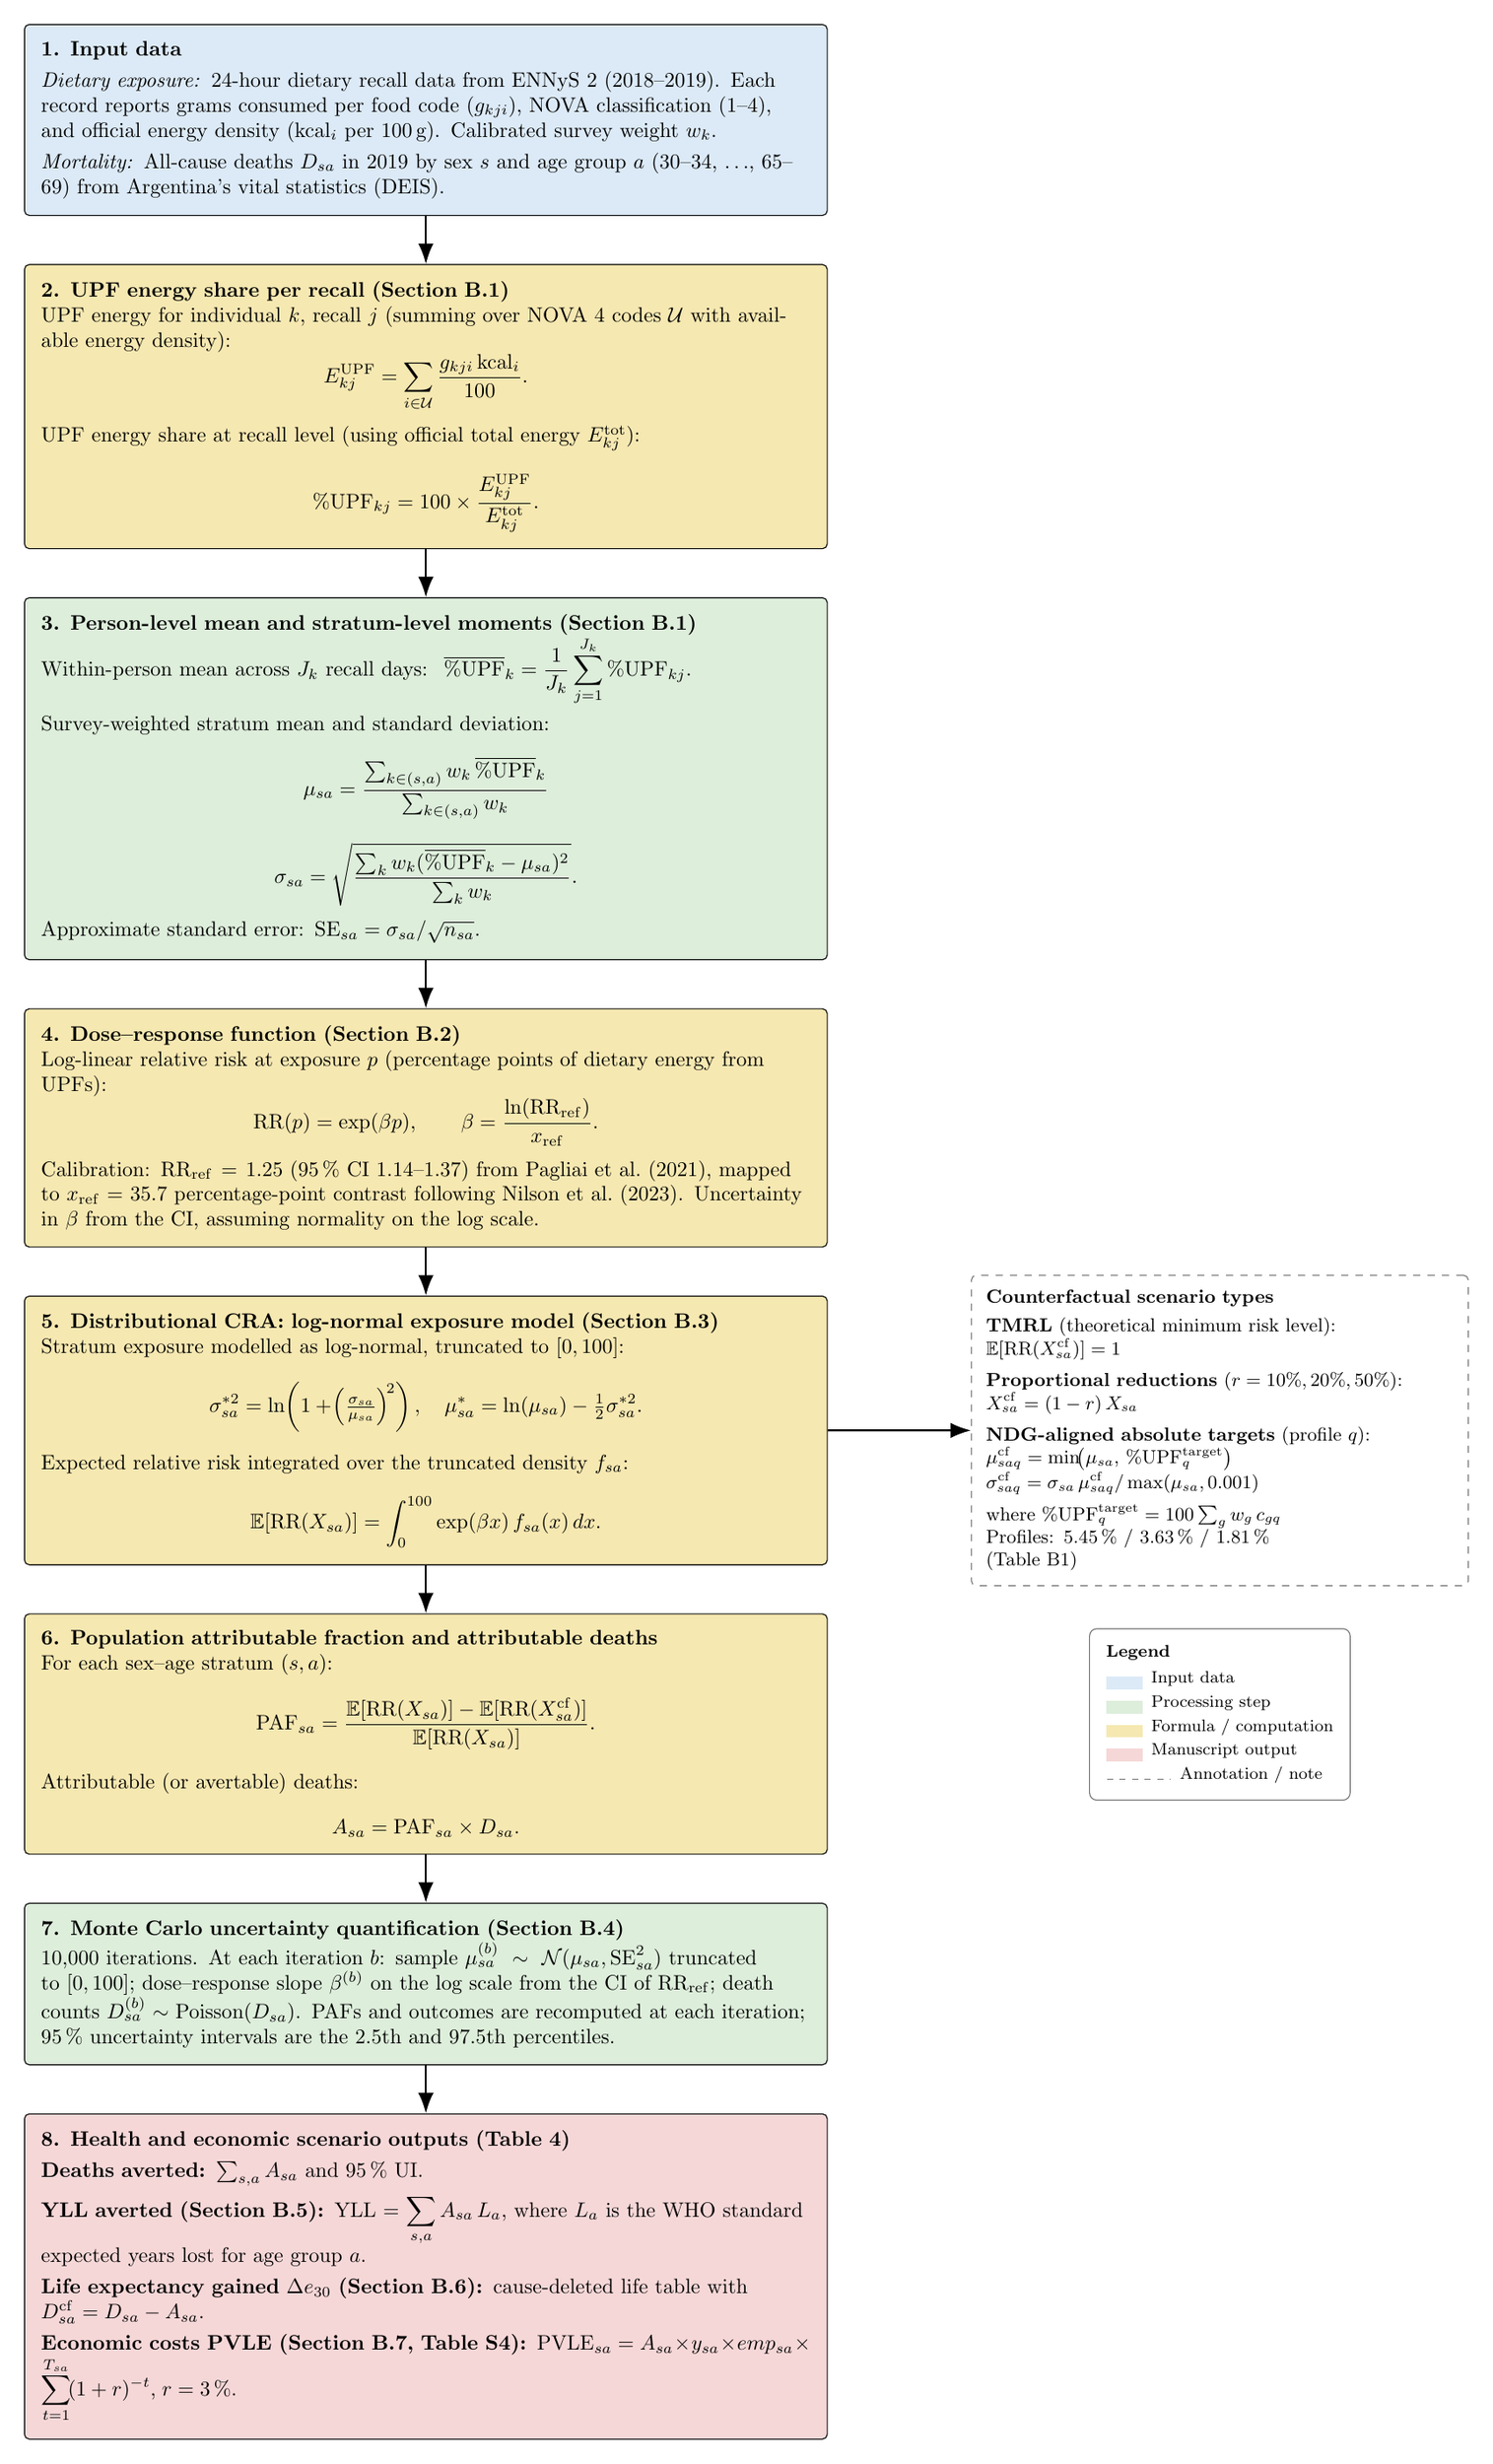
\begin{tikzpicture}[node distance=0.32in and 0.42in, scale=0.87, every node/.style={transform shape}]

\node[data] (input) at (0,0) {
\textbf{1. Input data}\\[3pt]
\textit{Dietary exposure:} 24-hour dietary recall data from ENNyS~2
(2018--2019). Each record reports grams consumed per food code
($g_{kji}$), NOVA classification (1--4), and official energy density
($\mathrm{kcal}_i$ per 100\,g). Calibrated survey weight $w_k$.\\[3pt]
\textit{Mortality:} All-cause deaths $D_{sa}$ in 2019 by sex $s$ and
age group $a$ (30--34, $\ldots$, 65--69) from Argentina's vital
statistics (DEIS).
};

\node[formula, below=of input] (exposure) {
\textbf{2. UPF energy share per recall (Section~B.1)}\\
UPF energy for individual $k$, recall $j$ (summing over NOVA~4 codes
$\mathcal{U}$ with available energy density):
\[
  E^{\mathrm{UPF}}_{kj}=\sum_{i\in\mathcal{U}}\frac{g_{kji}\,\mathrm{kcal}_i}{100}.
\]
UPF energy share at recall level (using official total energy
$E^{\mathrm{tot}}_{kj}$):
\[
  \%\mathrm{UPF}_{kj}=100\times\frac{E^{\mathrm{UPF}}_{kj}}{E^{\mathrm{tot}}_{kj}}.
\]
};

\node[process, below=of exposure] (stratum) {
\textbf{3. Person-level mean and stratum-level moments (Section~B.1)}\\
Within-person mean across $J_k$ recall days:
$\;\overline{\%\mathrm{UPF}}_{k}=\dfrac{1}{J_k}\displaystyle\sum_{j=1}^{J_k}\%\mathrm{UPF}_{kj}$.\\[4pt]
Survey-weighted stratum mean and standard deviation:
\[
  \mu_{sa}=\frac{\sum_{k\in(s,a)}w_k\,\overline{\%\mathrm{UPF}}_{k}}
                {\sum_{k\in(s,a)}w_k}
\]
\[
  \sigma_{sa}=\sqrt{\frac{\sum_{k}w_k(\overline{\%\mathrm{UPF}}_{k}-\mu_{sa})^2}
                         {\sum_{k}w_k}}.
\]
Approximate standard error: $\mathrm{SE}_{sa}=\sigma_{sa}/\sqrt{n_{sa}}$.
};

\node[formula, below=of stratum] (dr) {
\textbf{4. Dose--response function (Section~B.2)}\\
Log-linear relative risk at exposure $p$ (percentage points of
dietary energy from UPFs):
\[
  \mathrm{RR}(p)=\exp(\beta p),\qquad
  \beta=\frac{\ln(\mathrm{RR}_{\mathrm{ref}})}{x_{\mathrm{ref}}}.
\]
Calibration: $\mathrm{RR}_{\mathrm{ref}}=1.25$
(95\,\% CI 1.14--1.37) from Pagliai et~al.\ (2021), mapped to
$x_{\mathrm{ref}}=35.7$ percentage-point contrast following
Nilson et~al.\ (2023). Uncertainty in $\beta$ from the CI, assuming
normality on the log scale.
};

\node[formula, below=of dr] (cra) {
\textbf{5. Distributional CRA: log-normal exposure model (Section~B.3)}\\
Stratum exposure modelled as log-normal, truncated to $[0,100]$:
\[
  \sigma_{sa}^{*2}=\ln\!\left(1+\!\left(\tfrac{\sigma_{sa}}{\mu_{sa}}\right)^{\!2}\right),\quad
  \mu_{sa}^{*}=\ln(\mu_{sa})-\tfrac{1}{2}\sigma_{sa}^{*2}.
\]
Expected relative risk integrated over the truncated density $f_{sa}$:
\[
  \mathbb{E}\!\left[\mathrm{RR}(X_{sa})\right]=\int_0^{100}\exp(\beta x)\,f_{sa}(x)\,dx.
\]
};

\node[note, right=0.95in of cra] (scenarios) {
\textbf{Counterfactual scenario types}\\[3pt]
\textbf{TMRL} (theoretical minimum risk level):\\
$\mathbb{E}[\mathrm{RR}(X^{\mathrm{cf}}_{sa})]=1$\\[4pt]
\textbf{Proportional reductions} ($r=10\%,20\%,50\%$):\\
$X^{\mathrm{cf}}_{sa}=(1-r)\,X_{sa}$\\[4pt]
\textbf{NDG-aligned absolute targets} (profile $q$):\\
$\mu^{\mathrm{cf}}_{saq}=\min\!\bigl(\mu_{sa},\,\%\mathrm{UPF}^{\mathrm{target}}_q\bigr)$\\
$\sigma^{\mathrm{cf}}_{saq}=\sigma_{sa}\,\mu^{\mathrm{cf}}_{saq}/\max(\mu_{sa},0.001)$\\[4pt]
where $\%\mathrm{UPF}^{\mathrm{target}}_q=100\textstyle\sum_g w_g\,c_{gq}$\\
Profiles: 5.45\,\% / 3.63\,\% / 1.81\,\%\\
(Table~B1)
};

\node[formula, below=of cra] (paf) {
\textbf{6. Population attributable fraction and attributable deaths}\\
For each sex--age stratum $(s,a)$:
\[
  \mathrm{PAF}_{sa}=
  \frac{\mathbb{E}[\mathrm{RR}(X_{sa})]-\mathbb{E}[\mathrm{RR}(X^{\mathrm{cf}}_{sa})]}
       {\mathbb{E}[\mathrm{RR}(X_{sa})]}.
\]
Attributable (or avertable) deaths:
\[
  A_{sa}=\mathrm{PAF}_{sa}\times D_{sa}.
\]
};

\node[
  draw=black!55, rounded corners=3pt,
  align=left, inner sep=8pt, font=\footnotesize,
  below=0.28in of scenarios
] (legend) {
  \textbf{Legend}\\[3pt]
  \colorbox{FlowBlue}{\hphantom{~~~~}}\enspace Input data\\[2pt]
  \colorbox{FlowGreen}{\hphantom{~~~~}}\enspace Processing step\\[2pt]
  \colorbox{FlowYellow}{\hphantom{~~~~}}\enspace Formula / computation\\[2pt]
  \colorbox{FlowRed}{\hphantom{~~~~}}\enspace Manuscript output\\[2pt]
  \tikz[baseline=0pt]\draw[black!55,dashed,line width=0.7pt](0,0)--(0.42in,0);%
  \enspace Annotation / note
};

\node[process, below=of paf] (mc) {
\textbf{7. Monte Carlo uncertainty quantification (Section~B.4)}\\
10,000 iterations. At each iteration $b$: sample
$\mu^{(b)}_{sa}\sim\mathcal{N}(\mu_{sa},\mathrm{SE}_{sa}^2)$ truncated
to $[0,100]$; dose--response slope $\beta^{(b)}$ on the log scale
from the CI of $\mathrm{RR}_{\mathrm{ref}}$; death counts
$D^{(b)}_{sa}\sim\mathrm{Poisson}(D_{sa})$. PAFs and outcomes are
recomputed at each iteration; 95\,\% uncertainty intervals are
the 2.5th and 97.5th percentiles.
};

\node[output, below=of mc] (outputs) {
\textbf{8. Health and economic scenario outputs (Table~4)}\\[3pt]
\textbf{Deaths averted:}\enspace$\sum_{s,a}A_{sa}$ and 95\,\%~UI.\\[3pt]
\textbf{YLL averted (Section~B.5):}\enspace
  $\mathrm{YLL}=\displaystyle\sum_{s,a}A_{sa}\,L_a$,
  where $L_a$ is the WHO standard expected years lost for age group~$a$.\\[3pt]
\textbf{Life expectancy gained} $\Delta e_{30}$ \textbf{(Section~B.6):}
  cause-deleted life table with
  $D^{\mathrm{cf}}_{sa}=D_{sa}-A_{sa}$.\\[3pt]
\textbf{Economic costs PVLE (Section~B.7, Table~S4):}
  $\mathrm{PVLE}_{sa}=A_{sa}\!\times\!y_{sa}\!\times\!emp_{sa}
  \!\times\!\displaystyle\sum_{t=1}^{T_{sa}}\!(1+r)^{-t}$,\;$r=3\,\%$.
};

\draw[flow]      (input)    -- (exposure);
\draw[flow]      (exposure) -- (stratum);
\draw[flow]      (stratum)  -- (dr);
\draw[flow]      (dr)       -- (cra);
\draw[smallflow] (cra)      -- (scenarios);
\draw[flow]      (cra)      -- (paf);
\draw[flow]      (paf)      -- (mc);
\draw[flow]      (mc)       -- (outputs);

\end{tikzpicture}
}
\caption*{\textbf{Fig.~B1.} Health impact estimation pipeline. Blue = input data; green = processing step; yellow = formula/computation; red = manuscript output. Section and table references point to this appendix.}
\end{figure}

\clearpage

\begin{figure}[!htbp]
\centering
\resizebox{\textwidth}{!}{%
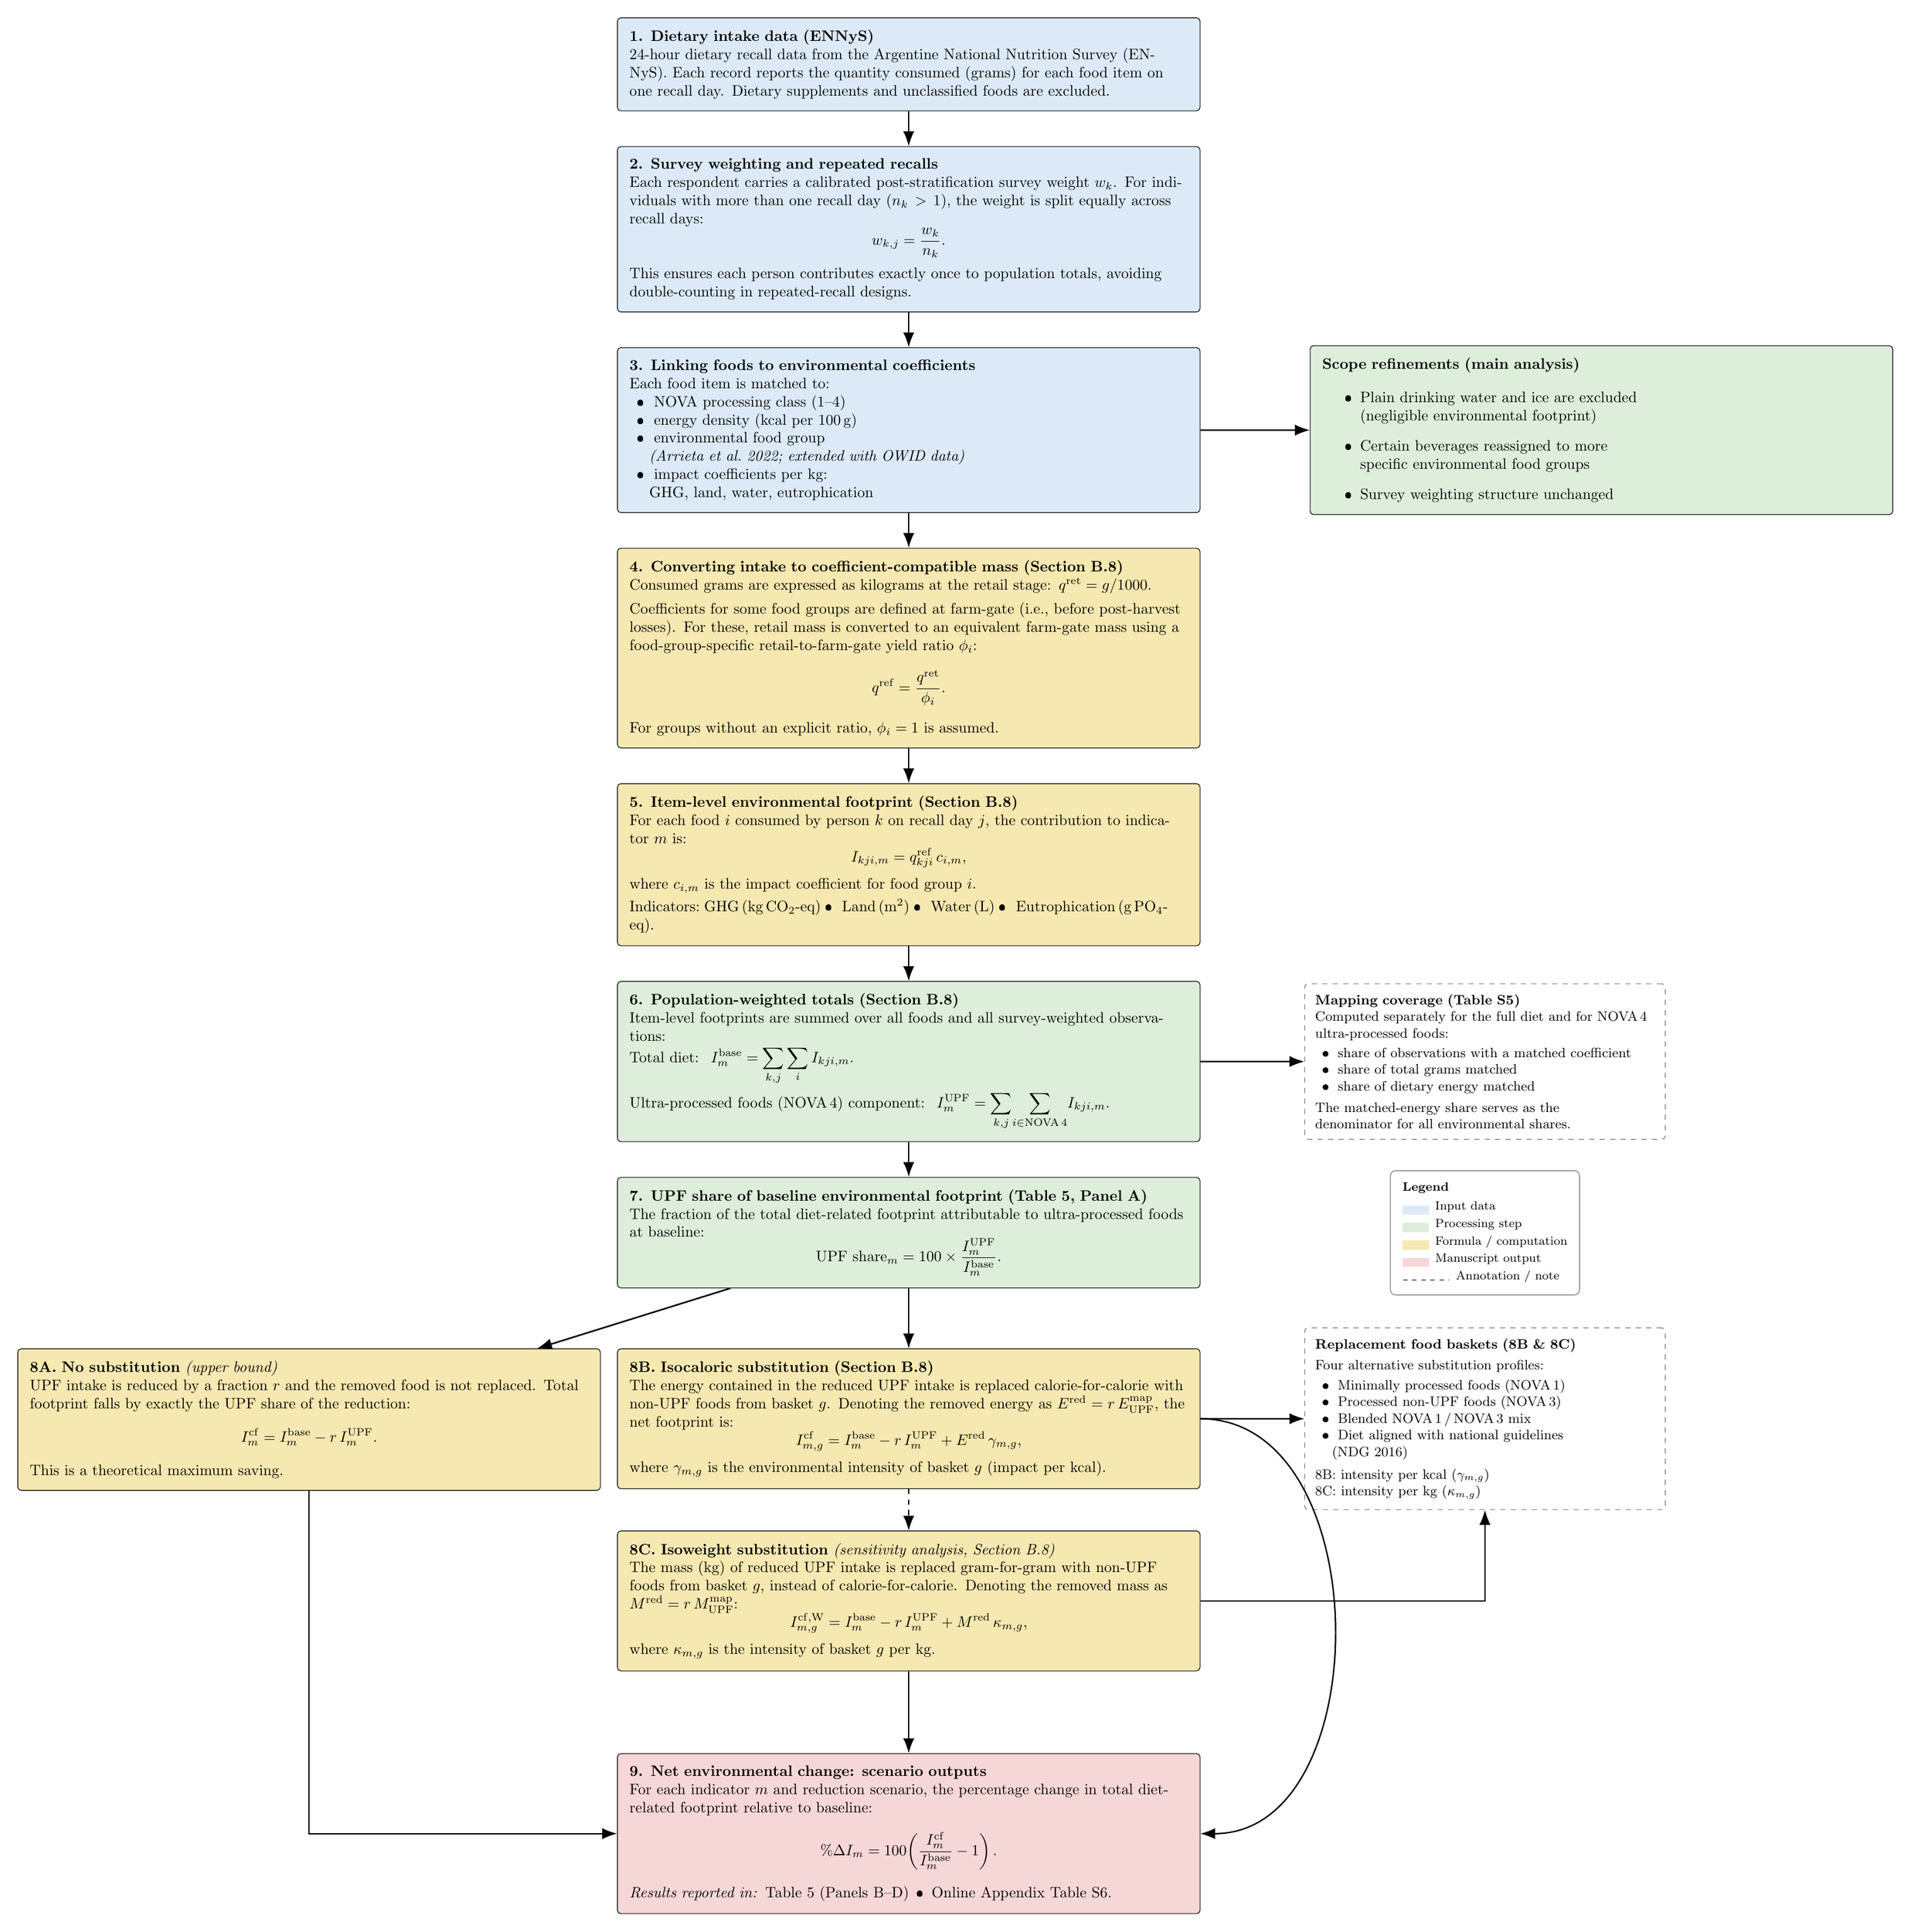
\begin{tikzpicture}[node distance=0.32in and 0.42in, scale=0.87, every node/.style={transform shape}]

\node[data] (input) at (0,0) {
\textbf{1. Dietary intake data (ENNyS)}\\
24-hour dietary recall data from the Argentine National Nutrition
Survey (ENNyS). Each record reports the quantity consumed (grams)
for each food item on one recall day. Dietary supplements and
unclassified foods are excluded.
};

\node[data, below=of input] (weights) {
\textbf{2. Survey weighting and repeated recalls}\\
Each respondent carries a calibrated post-stratification survey
weight~$w_k$. For individuals with more than one recall day ($n_k>1$),
the weight is split equally across recall days:
\[
  w_{k,j}=\frac{w_k}{n_k}.
\]
This ensures each person contributes exactly once to population totals,
avoiding double-counting in repeated-recall designs.
};

\node[data, below=of weights] (joins) {
\textbf{3. Linking foods to environmental coefficients}\\
Each food item is matched to:\\
\hspace*{0.5em}\textbullet\; NOVA processing class (1--4)\\
\hspace*{0.5em}\textbullet\; energy density (kcal per 100\,g)\\
\hspace*{0.5em}\textbullet\; environmental food group\\
\hspace*{1.3em}\textit{(Arrieta et~al.\ 2022; extended with OWID data)}\\
\hspace*{0.5em}\textbullet\; impact coefficients per kg:\\
\hspace*{1.3em}GHG, land, water, eutrophication
};

\node[process, right=1.0in of joins] (curated) {
\textbf{Scope refinements (main analysis)}\\
\begin{itemize}
  \item Plain drinking water and ice are excluded\\
        (negligible environmental footprint)
  \item Certain beverages reassigned to more\\
        specific environmental food groups
  \item Survey weighting structure unchanged
\end{itemize}
};

\node[formula, below=of joins] (mass) {
\textbf{4. Converting intake to coefficient-compatible mass (Section~B.8)}\\
Consumed grams are expressed as kilograms at the retail stage:
$q^{\mathrm{ret}}=g/1000$.\\[4pt]
Coefficients for some food groups are defined at farm-gate (i.e.,
before post-harvest losses). For these, retail mass is converted to
an equivalent farm-gate mass using a food-group-specific
retail-to-farm-gate yield ratio~$\phi_i$:
\[
  q^{\mathrm{ref}}=\frac{q^{\mathrm{ret}}}{\phi_i}.
\]
For groups without an explicit ratio, $\phi_i=1$ is assumed.
};

\node[formula, below=of mass] (itemimpact) {
\textbf{5. Item-level environmental footprint (Section~B.8)}\\
For each food~$i$ consumed by person~$k$ on recall day~$j$, the
contribution to indicator~$m$ is:
\[
  I_{kji,m}=q^{\mathrm{ref}}_{kji}\,c_{i,m},
\]
where $c_{i,m}$ is the impact coefficient for food group~$i$.\\[3pt]
Indicators:\;GHG\,(kg\,CO$_2$-eq)\;\textbullet\;
Land\,(m$^2$)\;\textbullet\;
Water\,(L)\;\textbullet\;
Eutrophication\,(g\,PO$_4$-eq).
};

\node[process, below=of itemimpact] (aggregate) {
\textbf{6. Population-weighted totals (Section~B.8)}\\
Item-level footprints are summed over all foods and all
survey-weighted observations:\\[2pt]
Total diet:\;
$\displaystyle I^{\mathrm{base}}_m=\sum_{k,j}\sum_i I_{kji,m}$.\\[4pt]
Ultra-processed foods (NOVA\,4) component:\;
$\displaystyle I^{\mathrm{UPF}}_m=\sum_{k,j}\!\sum_{i\in\mathrm{NOVA\,4}}\! I_{kji,m}$.
};

\node[note, right=0.95in of aggregate] (coverage) {
\textbf{Mapping coverage (Table~S5)}\\
Computed separately for the full diet and for NOVA\,4
ultra-processed foods:\\[2pt]
\hspace*{0.5em}\textbullet\; share of observations with a matched coefficient\\
\hspace*{0.5em}\textbullet\; share of total grams matched\\
\hspace*{0.5em}\textbullet\; share of dietary energy matched\\[3pt]
The matched-energy share serves as the\\
denominator for all environmental shares.
};

\node[
  draw=black!55, rounded corners=3pt,
  align=left, inner sep=8pt, font=\footnotesize,
  below=0.28in of coverage
] (legend2) {
  \textbf{Legend}\\[3pt]
  \colorbox{FlowBlue}{\hphantom{~~~~}}\enspace Input data\\[2pt]
  \colorbox{FlowGreen}{\hphantom{~~~~}}\enspace Processing step\\[2pt]
  \colorbox{FlowYellow}{\hphantom{~~~~}}\enspace Formula / computation\\[2pt]
  \colorbox{FlowRed}{\hphantom{~~~~}}\enspace Manuscript output\\[2pt]
  \tikz[baseline=0pt]\draw[black!55,dashed,line width=0.7pt](0,0)--(0.42in,0);%
  \enspace Annotation / note
};

\node[process, below=of aggregate] (shares) {
\textbf{7. UPF share of baseline environmental footprint (Table~5, Panel~A)}\\
The fraction of the total diet-related footprint attributable to
ultra-processed foods at baseline:
\[
  \text{UPF share}_m = 100\times\frac{I^{\mathrm{UPF}}_m}{I^{\mathrm{base}}_m}.
\]
};

\node[formula, below left=0.55in and 0.15in of shares] (norepl) {
\textbf{8A. No substitution} \normalfont\textit{(upper bound)}\\
UPF intake is reduced by a fraction~$r$ and the removed
food is not replaced. Total footprint falls by exactly the
UPF share of the reduction:
\[
  I^{\mathrm{cf}}_m = I^{\mathrm{base}}_m - r\,I^{\mathrm{UPF}}_m.
\]
This is a theoretical maximum saving.
};

\node[formula, below=0.55in of shares] (iso) {
\textbf{8B. Isocaloric substitution (Section~B.8)}\\
The energy contained in the reduced UPF intake is replaced
calorie-for-calorie with non-UPF foods from basket~$g$.
Denoting the removed energy as $E^{\mathrm{red}}=r\,E^{\mathrm{map}}_{\mathrm{UPF}}$,
the net footprint is:
\[
  I^{\mathrm{cf}}_{m,g}=I^{\mathrm{base}}_m-r\,I^{\mathrm{UPF}}_m
  +E^{\mathrm{red}}\,\gamma_{m,g},
\]
where $\gamma_{m,g}$ is the environmental intensity of basket~$g$
(impact per kcal).
};

\node[note, right=0.95in of iso] (baskets) {
\textbf{Replacement food baskets (8B \& 8C)}\\[3pt]
Four alternative substitution profiles:\\[2pt]
\hspace*{0.5em}\textbullet\; Minimally processed foods (NOVA\,1)\\
\hspace*{0.5em}\textbullet\; Processed non-UPF foods (NOVA\,3)\\
\hspace*{0.5em}\textbullet\; Blended NOVA\,1\,/\,NOVA\,3 mix\\
\hspace*{0.5em}\textbullet\; Diet aligned with national guidelines\\
\hspace*{1.2em}(NDG~2016)\\[4pt]
8B: intensity per kcal ($\gamma_{m,g}$)\\
8C: intensity per kg ($\kappa_{m,g}$)
};

\node[formula, below=0.38in of iso] (isoweight) {
\textbf{8C. Isoweight substitution}
\normalfont\textit{(sensitivity analysis, Section~B.8)}\\
The mass (kg) of reduced UPF intake is replaced gram-for-gram
with non-UPF foods from basket~$g$, instead of calorie-for-calorie.
Denoting the removed mass as $M^{\mathrm{red}}=r\,M^{\mathrm{map}}_{\mathrm{UPF}}$:
\[
  I^{\mathrm{cf,W}}_{m,g}=I^{\mathrm{base}}_m-r\,I^{\mathrm{UPF}}_m
  +M^{\mathrm{red}}\,\kappa_{m,g},
\]
where $\kappa_{m,g}$ is the intensity of basket~$g$ per kg.
};

\node[output, below=0.75in of isoweight] (outputs) {
\textbf{9. Net environmental change: scenario outputs}\\
For each indicator~$m$ and reduction scenario, the percentage change
in total diet-related footprint relative to baseline:
\[
  \%\Delta I_m = 100\!\left(\frac{I^{\mathrm{cf}}_m}{I^{\mathrm{base}}_m}-1\right).
\]
\textit{Results reported in:}\enspace
Table~5 (Panels~B--D)\enspace\textbullet\enspace
Online Appendix Table~S6.
};

\draw[flow]      (input)      -- (weights);
\draw[flow]      (weights)    -- (joins);
\draw[smallflow] (joins)      -- (curated);
\draw[flow]      (joins)      -- (mass);
\draw[flow]      (mass)       -- (itemimpact);
\draw[flow]      (itemimpact) -- (aggregate);
\draw[smallflow] (aggregate)  -- (coverage);
\draw[flow]      (aggregate)  -- (shares);
\draw[flow]      (shares)     -- (norepl);
\draw[flow]      (shares)     -- (iso);
\draw[smallflow] (iso)        -- (baskets);
\draw[smallflow, dashed] (iso) -- (isoweight);
\draw[smallflow] (isoweight.east) -| (baskets.south);
\draw[smallflow] (norepl.south)    |- (outputs.west);
\draw[smallflow] (iso.east) to[out=0,in=0,looseness=1.1] (outputs.east);
\draw[flow]      (isoweight)       -- (outputs);

\end{tikzpicture}
}
\caption*{\textbf{Fig.~B2.} Environmental footprint estimation pipeline.}
\end{figure}

\fi % end of repositioned figures

\appsubsection{Notation}
Sex is indexed by $s$, age group by $a$ (30--34, 35--39, \ldots, 65--69), individual by $k$, recall day by $j$, and food code by $i$. Calibrated survey weights are $w_k$. Observed deaths in stratum $(s,a)$ are $D_{sa}$ and UPF-attributable deaths are $A_{sa}$. The exposure is the dietary energy share from ultra-processed foods (UPFs), measured in percentage points from 0 to 100. Environmental indicators are indexed by $m$.

\appsubsection{B.1 Estimation of UPF contribution to total energy intake}
The exposure is defined as the percentage of total dietary energy from UPFs. First, UPF energy per recall is computed by summing item-level energy over food codes classified as NOVA~4 with official energy density available.
\[
E^{\mathrm{UPF}}_{kj}=\sum_{i\in\mathcal{U}}\frac{g_{kji}\,\mathrm{kcal}_i}{100},
\]
where $\mathcal{U}$ denotes the set of NOVA~4 food codes with available $\mathrm{kcal}_i$. \citep{Monteiro2019UPFIdentify,ENNYS22019}

Second, recall-level \%UPF uses the official total energy for that recall, $E^{\mathrm{tot}}_{kj}$, as denominator.
\[
\%\mathrm{UPF}_{kj}=100\times\frac{E^{\mathrm{UPF}}_{kj}}{E^{\mathrm{tot}}_{kj}}.
\]
Recalls with non-positive total energy or values outside $[0,100]$ are excluded.

Third, for participants with multiple recalls, we compute a within-person mean.
\[
\overline{\%\mathrm{UPF}}_{k}=\frac{1}{J_k}\sum_{j=1}^{J_k}\%\mathrm{UPF}_{kj}.
\]

Fourth, stratum-level summaries are computed as weighted moments.
\[
\mu_{sa}=\frac{\sum_{k\in(s,a)}w_k\,\overline{\%\mathrm{UPF}}_{k}}{\sum_{k\in(s,a)}w_k},\qquad
\sigma_{sa}=\sqrt{\frac{\sum_{k\in(s,a)}w_k\left(\overline{\%\mathrm{UPF}}_{k}-\mu_{sa}\right)^2}{\sum_{k\in(s,a)}w_k}}.
\]

Because full replicate-weight variance estimation was not available for all derived exposure moments, sampling uncertainty in $\mu_{sa}$ was propagated using an approximate standard error $\mathrm{SE}_{sa}=\sigma_{sa}/\sqrt{n_{sa}}$, where $n_{sa}$ is the number of individuals in the stratum. This approximation should be interpreted as capturing within-stratum sampling variability rather than the full complex-survey variance.

\appsubsection{B.2 Dose--response function and relative risk}
The CRA framework requires a continuous risk function to translate the full stratum-specific exposure distribution (not only mean exposure) into expected risk. For this reason, we parameterised the UPF--mortality association as a log-linear dose--response function in which risk increases multiplicatively with each additional percentage point of dietary energy from UPFs:
\[
\mathrm{RR}(p)=\exp(\beta p), \qquad \beta=\frac{\ln(\mathrm{RR}_{\mathrm{ref}})}{x_{\mathrm{ref}}}.
\]
The reference effect size was taken from the meta-analysis used in the main model input, $\mathrm{RR}_{\mathrm{ref}}=1.25$ (95\% CI 1.14--1.37) for all-cause mortality. \citep{Pagliai2021} To convert this pooled high-versus-low contrast into a continuous coefficient, we used the exposure contrast adopted in prior UPF CRA applications, $x_{\mathrm{ref}}=35.7$ percentage points of energy from UPFs (interpreted as an approximately 0\% to 35.7\% contrast). \citep{Nilson2023} This calibration imposes two anchors: $\mathrm{RR}(0)=1$ and $\mathrm{RR}(35.7)=1.25$, yielding $\beta=\ln(1.25)/35.7=0.00625$.

Under this specification, relative risk at any exposure level can be evaluated directly and integrated over the observed exposure distribution. For interpretation, a 10-percentage-point increase in UPF energy share corresponds to $\exp(10\beta)=1.064$, i.e., about a 6.4\% higher mortality risk under the model assumptions.

Uncertainty in $\beta$ was propagated from the reported confidence interval of $\mathrm{RR}_{\mathrm{ref}}$ by working on the log scale and assuming approximate normality of the log-risk coefficient, following standard burden-of-disease practice. \citep{WHO2024MethodsGBD} This uncertainty component was then sampled in the Monte Carlo stage (Section~B.4).

\appsubsection{B.3 Population attributable fraction (distributional CRA)}
Population attributable fractions (PAFs) were computed using a distributional comparative risk assessment approach, integrating risk over the exposure distribution within each stratum. \citep{WHO2024MethodsGBD,Nilson2023}

Within each stratum $(s,a)$, exposure was modelled as log-normal, parameterised from the stratum mean and standard deviation.
\[
X_{sa}\sim\mathrm{LogNormal}(\mu_{sa}^*,\sigma_{sa}^{*2}),
\qquad
\sigma_{sa}^{*2}=\ln\left(1+\left(\frac{\sigma_{sa}}{\mu_{sa}}\right)^2\right),\quad
\mu_{sa}^*=\ln(\mu_{sa})-\frac{\sigma_{sa}^{*2}}{2}.
\]
Because \%UPF is bounded, expectations were evaluated over $[0,100]$ using a truncated density.
\[
\mathbb{E}\!\left[\mathrm{RR}(X_{sa})\right]=\int_0^{100}\exp(\beta x)\,f_{sa}(x)\,dx,
\]
where $f_{sa}$ denotes the truncated log-normal density. \citep{WHO2024MethodsGBD}

For a proportional reduction scenario with fraction $r$, exposure is shifted to $X_{sa}^{\mathrm{cf}}=(1-r)X_{sa}$ and
\[
\mathrm{PAF}_{sa}=
\frac{\mathbb{E}[\mathrm{RR}(X_{sa})]-\mathbb{E}[\mathrm{RR}(X_{sa}^{\mathrm{cf}})]}
{\mathbb{E}[\mathrm{RR}(X_{sa})]}.
\]
For a theoretical minimum risk level (TMRL) at 0\% UPF, $\mathbb{E}[\mathrm{RR}(X_{sa}^{\mathrm{cf}})]=1$.

Guideline-aligned scenarios imposed absolute \%UPF targets derived from the National Dietary Guidelines (NDG) food-group structure. \citep{NDG2016} For profile $q\in\{\text{conservative},\text{central},\text{strict}\}$, the target was constructed as
\[
\%\mathrm{UPF}^{\mathrm{target}}_q = 100\sum_g w_g\,c_{gq},
\]
where $w_g$ are normalised NDG basket composition weights ($\sum_g w_g=1$) and $c_{gq}$ are group-specific residual UPF caps under profile $q$. Profile multipliers were defined as an exploratory $\pm50\%$ range around the central profile ($m_q\in\{1.5,1.0,0.5\}$), yielding targets of 5.45\% (conservative), 3.63\% (central), and 1.81\% (strict). For each stratum, we set the counterfactual mean to $\mu^{\mathrm{cf}}_{saq}=\min(\mu_{sa},\%\mathrm{UPF}^{\mathrm{target}}_q)$ and scaled the standard deviation proportionally, $\sigma^{\mathrm{cf}}_{saq}=\sigma_{sa}\,\mu^{\mathrm{cf}}_{saq}/\max(\mu_{sa},0.001)$, before recomputing $\mathbb{E}[\mathrm{RR}(X_{sa}^{\mathrm{cf}})]$.

Attributable deaths were then computed as $A_{sa}=\mathrm{PAF}_{sa}\,D_{sa}$ and summed over strata to obtain national totals. \citep{WHO2024MethodsGBD,Nilson2023}

\subsubsection*{Construction of group-specific UPF caps}
The central cap $c_g$ was set to reflect the maximum UPF fraction consistent with guideline-concordant consumption of that food group (Table~B1). Food groups where whole or minimally processed forms are normative---fruits, vegetables, legumes, rice, starchy vegetables, eggs, and nuts---were assigned $c_g=0$. Processed-grain groups (cereals, pasta), dairy products, and oil crops were assigned $c_g=0.10$, allowing a modest share of processed variants (e.g., packaged pasta, flavoured yoghurt) while maintaining guideline adherence. Baked products received $c_g=0.20$ because Argentina's guideline basket includes a small allowance for bread-type items, and NOVA~4 classification is common in this group. All animal-protein groups (meats, fish) were assigned $c_g=0.02$, a near-zero allowance consistent with fresh-cut or lightly processed preparations. The three profiles apply a uniform multiplier: $c_{gq}=\min(c_g\,m_q,\,0.95)$, where $m_{\mathrm{conservative}}=1.5$, $m_{\mathrm{central}}=1.0$, and $m_{\mathrm{strict}}=0.5$.

Because the NDG normative diet assigns large energy shares to plant-based groups that carry a zero cap---fruits (18\%), vegetables (25\%), and legumes (5\%)---the aggregated target is well below Argentina's observed UPF share of 16.66\%, producing reductions of 67.3\%, 78.2\%, and 89.1\% for the conservative, central, and strict profiles, respectively. The derivation of the 3.63\% central target is shown in Table~B1 and the scenario-level targets are summarised in Table~S7.

\vspace{0.5em}
\noindent\textbf{Table B1.} Derivation of the central NDG guideline-aligned UPF target (3.63\% energy)

\smallskip
\begin{center}
\small
\begin{tabular}{lrrr}
\toprule
\textbf{Food group} & \textbf{NDG weight $w_g$ (\%)} & \textbf{Central cap $c_g$} & \textbf{Contribution $w_g c_g$ (pp)} \\
\midrule
Fruits & 18.0 & 0.00 & 0.00 \\
Vegetables & 25.0 & 0.00 & 0.00 \\
Legumes and pulses & 5.0 & 0.00 & 0.00 \\
Cereals (excl.\ rice) & 6.0 & 0.10 & 0.60 \\
Rice & 3.0 & 0.00 & 0.00 \\
Pasta & 3.0 & 0.10 & 0.30 \\
Baked products & 3.0 & 0.20 & 0.60 \\
Starchy vegetables & 3.0 & 0.00 & 0.00 \\
Dairy products & 13.0 & 0.10 & 1.30 \\
Beef & 4.0 & 0.02 & 0.08 \\
Lamb and mutton & 0.5 & 0.02 & 0.01 \\
Other meats & 0.5 & 0.02 & 0.01 \\
Poultry & 2.5 & 0.02 & 0.05 \\
Pork & 1.0 & 0.02 & 0.02 \\
Fish and seafood & 3.0 & 0.02 & 0.06 \\
Eggs & 1.5 & 0.00 & 0.00 \\
Oil crops & 6.0 & 0.10 & 0.60 \\
Nuts and seeds & 2.0 & 0.00 & 0.00 \\
\midrule
\textbf{Total} & \textbf{100.0} & & \textbf{3.63} \\
\bottomrule
\end{tabular}
\end{center}

\noindent{\begingroup\footnotesize\setstretch{1}\selectfont NDG weights ($w_g$) are the normative energy shares prescribed by Argentina's 2016 National Dietary Guidelines. The central cap $c_g$ is the maximum UPF fraction assigned to each food group for a guideline-concordant dietary pattern; caps are scenario assumptions intended to reflect guideline intent rather than observed values. The population-level target equals $100\sum_g w_g c_g = 3.63\%$ of total dietary energy. Conservative (5.45\%) and strict (1.81\%) targets are obtained by multiplying all central caps by 1.5 and 0.5, respectively.\par\endgroup}

\vspace{0.5em}

\appsubsection{B.4 Monte Carlo uncertainty quantification}
Because attributable mortality is a nonlinear function of exposure, risk coefficients, and death counts, analytic variance propagation is not straightforward in this setting. We therefore used probabilistic Monte Carlo simulation to jointly propagate uncertainty from key model inputs and obtain uncertainty intervals for both stratum-level and national estimates, following standard comparative risk assessment practice. \citep{WHO2024MethodsGBD,Nilson2023}

We ran 10,000 iterations. For each stratum $(s,a)$ and iteration $b$, inputs were sampled as:
\[
\mu^{(b)}_{sa}\sim\mathcal{N}(\mu_{sa},\mathrm{SE}_{sa}^2),\qquad
\mu^{(b)}_{sa}\in[0.1,100],
\]
\[
\beta^{(b)}\sim\mathcal{N}(\beta,\mathrm{SE}_{\beta}^{2}),\qquad
D^{(b)}_{sa}\sim\mathrm{Poisson}(D_{sa}).
\]
Here, $\mu^{(b)}_{sa}$ is the sampled mean exposure, truncated to the feasible \%UPF range; $\beta^{(b)}$ is the sampled dose--response slope using the uncertainty derived from the confidence interval of the reference RR (Section~B.2); and $D^{(b)}_{sa}$ is a sampled death count under a Poisson counting model. The stratum-specific exposure spread ($\sigma_{sa}$) was held at its estimated value and used to evaluate the distributional PAF under each draw.

For each iteration, we recomputed baseline PAFs, attributable deaths, and scenario-specific avertable deaths using the same equations as in Section~B.3. Final point estimates are reported as medians (50th percentile), and uncertainty intervals as the 2.5th and 97.5th percentiles of the simulated distributions.

To complement deaths averted, we report two additional mortality-burden metrics: years of life lost (YLL) and life expectancy gained. YLL captures premature mortality by weighting attributable deaths by remaining standard life expectancy, and life expectancy gain translates those avoided deaths into an intuitive population-level metric at age 30. Both measures follow standard WHO/GBD burden-of-disease conventions, improving comparability across studies and policy scenarios. \citep{Murray2003,WHO2024MethodsGBD}

\appsubsection{B.5 Years of life lost (YLL)}
YLL was estimated to capture the timing of premature mortality attributable to UPF intake, not only the number of attributable deaths. Death counts alone treat deaths at different ages as equivalent, while YLL assigns larger weight to deaths that occur earlier in adult life. This improves interpretability for prevention policy and keeps results comparable with WHO/GBD burden metrics. \citep{Murray2003,WHO2024MethodsGBD}

For each sex-age stratum, YLL is
\[
\mathrm{YLL}_{sa}=A_{sa}\,L_a,
\]
and national YLL is
\[
\mathrm{YLL}=\sum_{s,a}A_{sa}\,L_a,
\]
where $A_{sa}$ are UPF-attributable deaths from the comparative risk assessment model (Sections~B.2--B.4), and $L_a$ denotes standard remaining life expectancy at age group $a$ from the WHO reference table. \citep{Murray2003,WHO2024MethodsGBD}

In implementation, age-specific YLL weights were fixed for the 30--69 year groups (30--34: 60.34; 35--39: 55.38; 40--44: 50.43; 45--49: 45.51; 50--54: 40.61; 55--59: 35.74; 60--64: 30.92; 65--69: 26.21 years). These weights were applied identically across sexes, consistent with WHO/GBD practice of using a common standard life table for comparability.

No additional age weighting or time discounting was applied to YLL; burden differences are driven only by the number of attributable deaths and the standard life-years remaining in each age group.

Uncertainty was propagated at each Monte Carlo draw by recomputing
\[
\mathrm{YLL}^{(b)}=\sum_{s,a}A_{sa}^{(b)}L_a.
\]
For each scenario $q$, avertable YLL was computed as
\[
\Delta \mathrm{YLL}^{(q,b)}=\sum_{s,a}A^{(q,b)}_{sa}L_a,
\]
and final results were summarized as the median and 95\% uncertainty interval (2.5th--97.5th percentiles) across draws (Section~B.4).

\appsubsection{B.6 Life expectancy gained (cause-deleted life table)}
Life expectancy gain was included as a complementary mortality metric because it translates avertable deaths into expected years lived from age 30 under observed mortality conditions. In this framework, YLL quantifies the burden removed, whereas the cause-deleted life table expresses the same removal as a shift in survival expectancy. This is a standard comparative risk assessment approach. \citep{Murray2003,WHO2004CQR,Forouzanfar2015,WHO2024MethodsGBD}

A baseline life table was built from observed deaths and population in 5-year age bands (30--34 to 65--69). For each stratum, baseline central mortality was
\[
m_{sa}=\frac{D_{sa}}{N_{sa}}.
\]
Age-specific death probabilities were then obtained using the standard abridged conversion
\[
q_x=\frac{n\,m_x}{1+\frac{n}{2}m_x},\qquad n=5,
\]
with a radix of $l_{30}=100{,}000$. Survivors and deaths were updated recursively by $d_x=l_xq_x$ and $l_{x+n}=l_x-d_x$. Person-years in each interval were computed as
\[
L_x=n\,l_{x+n}+\frac{n}{2}d_x,
\]
then accumulated as $T_x=\sum_{y\ge x}L_y$, and life expectancy obtained as $e_x=T_x/l_x$.

For the final open interval, a terminal-life assumption was applied using expected years at age 70 of $E_{70}=18.5$, so that the last age-group contribution includes survivors beyond 69 years.

The counterfactual removes UPF-attributable deaths,
\[
D^{\mathrm{cf}}_{sa}=D_{sa}-A_{sa},\qquad
m^{\mathrm{cf}}_{sa}=\frac{D^{\mathrm{cf}}_{sa}}{N_{sa}},
\]
and recomputes all life-table functions under the same assumptions. Life expectancy gain at age 30 is
\[
\Delta e_{30}=e_{30}^{\mathrm{cf}}-e_{30}.
\]
For scenario reporting, $A_{sa}$ is replaced by scenario-specific avertable deaths $A^{(q)}_{sa}$, yielding $\Delta e_{30}^{(q)}$ for each policy target.

This cause-deleted construction assumes that removing UPF-attributable deaths changes all-cause mortality only through the deleted component, while other-cause hazards within each stratum remain unchanged. Under that assumption, the estimated $\Delta e_{30}$ can be interpreted as a partial expectancy gain attributable to the modelled UPF mortality component in ages 30--69, rather than as a full forecast of national life expectancy dynamics.

Uncertainty in $\Delta e_{30}$ was propagated by repeating the entire cause-deleted life table calculation at each Monte Carlo draw using $A_{sa}^{(b)}$ (or $A_{sa}^{(q,b)}$ for scenarios), and summarizing the resulting distribution with medians and 95\% uncertainty intervals.

\appsubsection{B.7 Indirect economic costs (human capital approach)}
Indirect costs were included because mortality burden also implies loss of productive years, not only health loss. We used the human capital approach, in which each premature death is valued as the discounted stream of expected labour earnings that would have occurred until retirement age. This approach is widely used in burden studies when the objective is to estimate the full production value forgone from premature mortality, and it is aligned with reference-case guidance when productivity effects are reported from a societal perspective. \citep{Sanders2016SecondPanel,iDSIReferenceCase2014}

For each stratum $(s,a)$, indirect costs were valued as the present value of forgone earnings until an assumed retirement age of 65 years for both sexes:
\[
\mathrm{PVLE}_{sa}=A_{sa}\times y_{sa}\times emp_{sa}\times \sum_{t=1}^{T_{sa}}(1+r)^{-t},
\]
where $y_{sa}$ is mean annual labour income, $emp_{sa}$ is the employment rate, $r=0.03$ is the discount rate, and $T_{sa}$ is remaining working years from the age-group midpoint (capped at zero). The annuity factor is
\[
\sum_{t=1}^{T}(1+r)^{-t}=\frac{1-(1+r)^{-T}}{r}.
\]
Age-midpoint mapping implies $T_{sa}=0$ for 65--69 years, so deaths in that group contribute no additional labour-market losses under this framework.

In Argentina, statutory retirement ages are generally 60 years for women and 65 years for men; we used a uniform age-65 horizon as a simplifying assumption to apply a common valuation window across strata. \citep{ANSESJubilacionOrdinaria2026} The 3\% annual discount rate follows reference-case guidance. \citep{iDSIReferenceCase2014,Sanders2016SecondPanel} Income and employment inputs were derived from national labour survey microdata (monthly income annualised by $\times12$), and monetary totals were converted from ARS to intl.\$ using the 2019 PPP factor (20.38 ARS/intl.\$). \citep{INDECEPH2019Q4,INDECMercadoTrabajo2020,WorldBankPPP2019}

The valuation is static and incidence-based: wages and employment rates are held at their observed 2019 stratum-specific values, with no additional assumptions on future wage growth, labour-force transitions, or macroeconomic feedback effects. Therefore, estimates should be interpreted as discounted market-income losses directly linked to modelled premature deaths under the observed labour market structure.

For each scenario $q$, avertable indirect cost was computed by replacing $A_{sa}$ with $A^{(q)}_{sa}$ and summing over strata:
\[
\Delta \mathrm{PVLE}^{(q)}=\sum_{s,a}A^{(q)}_{sa}\,y_{sa}\,emp_{sa}\,\frac{1-(1+r)^{-T_{sa}}}{r}.
\]
Uncertainty was propagated by applying the same valuation equation to each simulation draw $A_{sa}^{(q,b)}$ and summarizing medians and 95\% uncertainty intervals.

This specification captures market labour losses only. It does not include unpaid household production, caregiver time, employer replacement dynamics (friction-cost adjustments), or intangible welfare losses beyond labour income.

\appsubsection{B.8 Environmental impacts, replacement matrix, and structural sensitivities}
Environmental impacts were not assigned by building a separate life-cycle inventory for each ENNyS food code. Instead, each consumed ENNyS food code was linked through a mapping dictionary to an environmental food group, and group-level coefficients were then applied. Thus, multiple ENNyS codes can share the same environmental coefficient set. The environmental analysis used four indicators at the food-group level: greenhouse gas emissions (kg CO$_2$-eq), land use (m$^2$), water use (L), and freshwater eutrophication (g PO$_4$-eq) per kg of reference mass. \citep{Arrieta2022SustainSci,PooreNemecek2018,OWIDDatasets2026,ADEMEAgribalyse2026}

For each individual $k$, recall day $j$, and food code $i$, reported grams were first transformed into weighted population-representative quantities using the calibrated survey weight and dividing that weight by the number of recalls available for the same person. This yields weighted grams and weighted energy that can be aggregated without double counting repeated recalls. Positive-intake records were then linked to their NOVA group, environmental group, and energy density before impact coefficients were applied.

For each food code $i$ and environmental indicator $m$, baseline item-level impact is
\[
I_{kji,m}=q_{kji}^{\mathrm{ref}}\;c_{i,m},
\]
where $q_{kji}^{\mathrm{ref}}$ is the reference mass (kg) consistent with the coefficient definition and $c_{i,m}$ is the impact coefficient per kg. The term ``reference mass'' means the mass expressed in the same physical reference used by the environmental coefficient. This matters because intake is observed at the retail/consumption level in ENNyS, whereas some coefficients are defined at farm-gate level. When coefficients are defined at farm-gate level and observed quantities are recorded at retail level, mass is converted using a yield factor $y_i$ (retail weight per farm weight).
\[
q_{kji}^{\mathrm{ref}}=\frac{q_{kji}^{\mathrm{ret}}}{y_i}.
\]
In practice, observed grams are first converted to retail kg and then, where necessary, to the mass reference required by the coefficient before multiplication by the corresponding per-kg impact factor. Baseline totals are then obtained by summing item-level impacts over all weighted records,
\[
I_m^{\mathrm{base}}=\sum_{k,j}\sum_i I_{kji,m},
\]
and the UPF component is computed by restricting the same sum to NOVA~4 codes,
\[
I_m^{\mathrm{UPF}}=\sum_{k,j}\sum_{i\in \mathrm{NOVA4}} I_{kji,m}.
\]

The manuscript reports results from the environmental specification used for the main tables. In that specification, plain drinking water and ice were excluded from the environmental scope, because they dominate grams consumed but contribute no dietary energy, and selected beverages without a direct comparable-group match were reassigned to more appropriate beverage groups before coefficients were applied (e.g., mate/yerba, tea or infusions, coffee, industrial fruit juice, flavoured water, beer, wine, and spirits). Coverage diagnostics for this mapping are shown in Table~S5. In this in-scope analysis, row-level mapping coverage was lower than gram- and energy-level coverage, but mapped energy coverage was high overall and within NOVA~4.

\paragraph*{Counterfactual accounting.}
Counterfactual scenarios apply the same UPF-reduction fractions used in the health analysis (10\%, 20\%, 50\%, and the NDG-aligned targets), denoted here by $r$. For each environmental indicator $m$, the accounting logic is the same in all scenarios: we first calculate the gross impact removed by reducing UPFs, then add back the impact of any replacement basket when substitution is assumed, and finally compare the resulting counterfactual total with the observed baseline.

Let the gross removed impact be
\[
I^{\mathrm{rem}}_{m}=r\,I^{\mathrm{UPF}}_{m}.
\]
Under no substitution, a fraction $r$ of the UPF component is removed and nothing is added back. The counterfactual therefore becomes
\[
I^{\mathrm{cf}}_{m}=I^{\mathrm{base}}_{m}-r\,I^{\mathrm{UPF}}_{m}.
\]
This scenario can be interpreted as a mechanical upper bound, because the removed UPF component is not replaced by any other food or beverage.

Under isocaloric substitution, the model removes a fraction $r$ of mapped UPF intake but then restores the same amount of dietary energy using a non-UPF replacement basket. Let
\[
E^{\mathrm{red}}=r\,E^{\mathrm{map}}_{\mathrm{UPF}}
\]
denote removed mapped UPF energy. For a replacement basket $g$, define the basket intensity per kcal as
\[
\gamma_{m,g}=I_{m,g}/E_g,
\]
that is, environmental impact per kcal of the replacement basket. The impact added back by replacement is
\[
I^{\mathrm{add}}_{m,g}=E^{\mathrm{red}}\gamma_{m,g},
\]
and the counterfactual total is
\[
I^{\mathrm{cf}}_{m,g}=I^{\mathrm{base}}_{m}-r\,I^{\mathrm{UPF}}_{m}+I^{\mathrm{add}}_{m,g}.
\]
In words, the net environmental effect under isocaloric substitution is the impact of the removed UPF energy minus the impact of the calories used to replace it. A basket with lower impact per kcal than the removed UPFs will generate a net reduction, whereas a basket with higher impact per kcal can attenuate or reverse that reduction.

As an alternative substitution structure, we also implemented isoweight substitution, replacing removed UPF mass one-for-one rather than replacing calories one-for-one. Let
\[
M^{\mathrm{red}}=r\,M^{\mathrm{map}}_{\mathrm{UPF}}
\]
denote removed mapped UPF mass. For basket $g$, define impact intensity per kg as
\[
\kappa_{m,g}=I_{m,g}/M_g.
\]
The impact added back under mass-for-mass replacement is
\[
I^{\mathrm{add,kg}}_{m,g}=M^{\mathrm{red}}\kappa_{m,g},
\]
and the resulting counterfactual is
\[
I^{\mathrm{cf,W}}_{m,g}=I^{\mathrm{base}}_{m}-r\,I^{\mathrm{UPF}}_{m}+I^{\mathrm{add,kg}}_{m,g}.
\]
Because many non-UPF foods are less energy-dense than UPFs, isocaloric and isoweight substitution need not lead to the same environmental pattern.

We report environmental outcomes as net percentage change versus baseline,
\[
\%\Delta I_{m}=100\left(\frac{I^{\mathrm{cf}}_{m}}{I^{\mathrm{base}}_{m}}-1\right),
\]
so negative values indicate reductions and positive values indicate increases. Replacement baskets include NOVA~1, NOVA~3, a weighted NOVA~1/NOVA~3 mix, and an NDG-concordant basket. The NOVA~1 and NOVA~3 baskets use observed mapped non-UPF foods in those NOVA classes to estimate impact intensities. The weighted NOVA~1/NOVA~3 mix interpolates between those two structures using their observed mapped energy shares. The NDG-concordant basket uses food-group weights derived from the Argentine National Dietary Guidelines (NDG) together with observed mapped non-UPF foods to construct basket-specific impact intensities. The diet composition of these replacement baskets and the UPF targets used in the counterfactuals are summarised in Table~S7. NOVA~2 was not used as a standalone replacement basket because its units and scope are not directly comparable to foods in diet-based footprint accounting. \citep{NDG2016}


\appsection{Appendix C. Supplementary tables}
Tables~S1--S8 summarise key inputs and supplementary results that are not duplicated in the main manuscript. Additional granular scenario outputs and mapping files are included in the project materials.

\vspace{0.8em}
\begin{table}[!htbp]
\centering
\manualtablecaption{Table S1. Data sources summary}
\begin{tabular}{p{5.1cm}p{6.8cm}p{3.4cm}}
\toprule
\textbf{Input} & \textbf{Source} & \textbf{Year / resolution}\\
\midrule
Dietary intake (24h recalls) & ENNyS 2, Ministry of Health \citep{ENNYS22019} & 2018--2019 / individual\\
NOVA processing classification & NOVA framework \citep{Monteiro2019UPFIdentify} & food-code level\\
Relative risks (all-cause mortality) & Meta-analysis estimate with CRA calibration implementation \citep{Pagliai2021,Nilson2023} & published studies\\
Mortality counts by sex and age & Argentina vital statistics inputs; CRA framework \citep{DEIS2019,WHO2024MethodsGBD,Nilson2023} & 2019 / strata\\
Economic inputs (income, employment) & National household survey microdata \citep{INDECEPH2019Q4} & 2019 / strata\\
PPP conversion factor & World Bank \citep{WorldBankPPP2019} & 2019\\
Environmental coefficients & LCA sources and global datasets \citep{Arrieta2022SustainSci,PooreNemecek2018,OWIDDatasets2026,ADEMEAgribalyse2026} & food-group level\\
\bottomrule
\end{tabular}
\tabnote{CRA denotes comparative risk assessment, PPP denotes purchasing power parity, and LCA denotes life-cycle assessment.}
\end{table}

\clearpage
\setlength{\LTleft}{\fill}
\setlength{\LTright}{\fill}
{\footnotesize
\setlength{\tabcolsep}{4pt}
\begin{longtable}{p{4.3cm}p{5.5cm}p{1.5cm}p{0.7cm}}
\multicolumn{4}{l}{\textbf{Table S2. NOVA classification of ENNyS food and beverage codes}}\\
\toprule
\textbf{Item description (Spanish)} & \textbf{Item description (English)} & \textbf{Code} & \textbf{NOVA}\\
\midrule
\endfirsthead
\multicolumn{4}{l}{\textbf{Table S2. NOVA classification of ENNyS food and beverage codes (continued)}}\\
\toprule
\textbf{Item description (Spanish)} & \textbf{Item description (English)} & \textbf{Code} & \textbf{NOVA}\\
\midrule
\endhead
\midrule
\multicolumn{4}{r}{\emph{Continued on next page}}\\
\endfoot
\bottomrule
\endlastfoot
\multicolumn{4}{l}{\textbf{NOVA 1. Unprocessed or minimally processed foods}}\\
Abadejo & Pout & P029 & 1\\
Acelga & Chard & V001 & 1\\
Acelga, congelada & Chard, frozen & V050 & 1\\
Acelga, pencas & Chard, stalks & V073 & 1\\
Acerola & Acerola cherry & F044 & 1\\
Achicoria & Chicory & V002 & 1\\
Achilate / achilata & Achilate / achilata drink & B055 & 1\\
Agua con gas / soda & Sparkling water/soda & B111 & 1\\
Agua de lluvia, río, canal, arroyo o acequia & Rainwater, river, canal, stream or ditch & B109 & 1\\
Agua de lluvia, río, canal, arroyo o acequia, hervida y/o con lavandina & Rainwater, river, canal, stream or ditch, boiled and/or with bleach & B110 & 1\\
Agua de mar & Seawater & B126 & 1\\
Agua de perforación con bomba & Borehole water (pumped) & B105 & 1\\
Agua de perforación con bomba, hervida y/o con lavandina & Borehole water (pumped), boiled and/or chlorinated (bleach) & B106 & 1\\
Agua de pozo & Well water & B107 & 1\\
Agua de pozo, hervida y/o con lavandina & Well water, boiled and/or with bleach & B108 & 1\\
Agua de red pública o agua corriente, dentro del hogar & Public mains tap water, in-home & B101 & 1\\
Agua de red pública o agua corriente, filtrada (filtro o dispenser de agua) & Public mains tap water, filtered (filter/dispenser) & B102 & 1\\
Agua embotellada (bidón / botella) & Bottled water (jerrycan/bottle) & B103 & 1\\
Agua embotellada (bidón / botella), bajo contenido de sodio & Bottled water (jerrycan/bottle), low sodium & B104 & 1\\
Agua origen desconocido & Water, source unknown & B100 & 1\\
Aguja & Chuck steak (aguja cut) & C078 & 1\\
Ají Locoto & Rocoto chili pepper (locoto) & V077 & 1\\
Ají rojo / morrón rojo & Red chili / red bell pepper & V003 & 1\\
Ají verde o amarillo / morrón verde o amarillo & Green or yellow chili pepper / green or yellow bell pepper & V004 & 1\\
Ajo & Garlic & V065 & 1\\
Albahaca & Basil & V071 & 1\\
Alcaucil & Artichoke & V005 & 1\\
Almeja & Clam & P042 & 1\\
Almendra & Almond & Z008 & 1\\
Amaranto & Amaranth & A002 & 1\\
Ananá & Pineapple & F003 & 1\\
Apio & Celery & V006 & 1\\
Arándanos & Blueberries & F060 & 1\\
Arroz blanco & White rice & A003 & 1\\
Arroz integral & Brown rice & A004 & 1\\
Arroz yamaní & Yamani rice & A102 & 1\\
Arveja, congelada & Pea, frozen & V051 & 1\\
Arveja, fresca & Pea, fresh & V007 & 1\\
Arveja, semilla seca entera / partida & Pea, dried whole/split seed & A006 & 1\\
Asado con hueso*** & Roast with bone*** & C076 & 1\\
Asado sin hueso*** & Boneless roast*** & C075 & 1\\
Atún, lomito fresco & Tuna, fresh loin & P028 & 1\\
Avellana & Hazelnut & Z009 & 1\\
Avena, arrollada & Oats, rolled & A005 & 1\\
Banana & Banana & F006 & 1\\
Banana deshidratada & Dehydrated banana & F067 & 1\\
Batata & Sweet potato & A073 & 1\\
Berenjena & Eggplant & V010 & 1\\
Berro & Watercress & V011 & 1\\
Bife angosto con hueso*** & Striploin steak, bone-in*** & C089 & 1\\
Bife angosto sin hueso*** & Striploin steak, boneless*** & C088 & 1\\
Bola de lomo & Eye of round & C082 & 1\\
Brócoli & Broccoli & V012 & 1\\
Brotes de soja & Soybean sprouts & V013 & 1\\
Brótola & Brotola & P021 & 1\\
Caballa, tronco & Mackerel, trunk & P011 & 1\\
Cabra & Goat & C001 & 1\\
Café en saquitos (ingresar cantidad de saquitos)* & Coffee in bags (enter number of bags)* & B073 & 1\\
Café preparado a partir de grano molido (tipo café de filtro) & Coffee prepared from ground beans (filter coffee type) & B058 & 1\\
Calamar & Squid & P003 & 1\\
Caldo de verduras colado & Strained vegetable broth & V082 & 1\\
Camarón & Shrimp & P004 & 1\\
Caracú & Beef marrow bone (caracú) & C109 & 1\\
Carne picada común & Regular ground beef & C073 & 1\\
Carne picada especial & Lean ground beef & C074 & 1\\
Carpincho & Capybara & C050 & 1\\
Cayota o Alcayota & Cayota or Alcayota & F045 & 1\\
Cebolla & Onion & V014 & 1\\
Cebolla de verdeo & Green onion & V052 & 1\\
Cerdo bondiola & Pork neck (bondiola) & C100 & 1\\
Cerdo costillar tipo "ribs" & Pork spare ribs & C099 & 1\\
Cerdo costillita & Pork short ribs & C098 & 1\\
Cerdo jamón (corte de carne) & Pork leg/fresh ham (cut of meat) & C104 & 1\\
Cerdo matambre & Pork flank (matambre) & C101 & 1\\
Cerdo paleta (corte de carne) & Pork shoulder (cut of meat) & C105 & 1\\
Cerdo pechito & Pork belly & C102 & 1\\
Cerdo, patas, patitas & Pork trotters & C115 & 1\\
Cerdo, PROMEDIO & Pork, AVERAGE & C002 & 1\\
Cereza & Cherry & F007 & 1\\
Champignones, frescos & Mushrooms, fresh & V076 & 1\\
Charata (ave) & Charata (bird) & C064 & 1\\
Chaucha, congelada & Green beans, frozen & V053 & 1\\
Chaucha, fresca & Green beans, fresh & V016 & 1\\
Chinchulines, tripa gorda & Chitterlings (small intestines), large intestine & C007 & 1\\
Chivito & Goat kid meat & C110 & 1\\
Chivito, cabeza & Chivito, head & C129 & 1\\
Choclo & Corn & A076 & 1\\
Choclo, congelado en grano & Corn, frozen grain & A176 & 1\\
Chuchu o chayote & Chuchu or chayote & V078 & 1\\
Ciruela & Plum & F008 & 1\\
Ciruela pasa / ciruela seca & Prune / dried plum & F009 & 1\\
Coco fresco & Fresh coconut & F046 & 1\\
Coco, leche & Coconut, milk & F066 & 1\\
Coliflor & Cauliflower & V015 & 1\\
Colita de cuadril & Rump tail (colita de cuadril) & C093 & 1\\
Conejo & Rabbit & C008 & 1\\
Corazón, vacuno & Heart, beef & C107 & 1\\
Cordero, PROMEDIO & Lamb, AVERAGE & C009 & 1\\
Cornalitos & Cornalitos (small silverside fish) & P031 & 1\\
Corvina & Croaker & P023 & 1\\
Cous Cous & Couscous & A118 & 1\\
Cuadrada & Cuadrada (beef bottom round) & C084 & 1\\
Cuadril & Rump (cuadril) & C092 & 1\\
Cuerito de cerdo & Pig skin & C052 & 1\\
Damasco & Apricot & F010 & 1\\
Dátiles & Dates & F061 & 1\\
Dorado & Golden dorado (river fish) & P035 & 1\\
Durazno & Peach & F011 & 1\\
Durazno orejón & Dried peach & F014 & 1\\
Escarola & Endive & V020 & 1\\
Espárrago & Asparagus & V021 & 1\\
Espinaca & Spinach & V022 & 1\\
Espinazo, vacuno & Backbone, beef & C120 & 1\\
Falda & Skirt/plate steak (falda) & C079 & 1\\
Frambuesa & Raspberry & F064 & 1\\
Frutilla & Strawberry & F015 & 1\\
Garbanzos & Chickpeas & A025 & 1\\
Garza & Heron & C062 & 1\\
Gatuzo & Smoothhound shark (gatuzo) & P024 & 1\\
Gérmen de trigo & Wheat germ & A129 & 1\\
Granada & Pomegranate & F016 & 1\\
Guabirova & Guabiroba (native berry) & F053 & 1\\
Guanaco, carne & Guanaco, meat & C111 & 1\\
Guayaba & Guava & F017 & 1\\
Habas & Broad beans & V023 & 1\\
Hakusai o col china & Hakusai or Chinese cabbage & V054 & 1\\
Hielo para bebidas & Ice for drinks & B114 & 1\\
Hígado & Liver & C012 & 1\\
Hígado de pollo & Chicken liver & C122 & 1\\
Higo & Fig & F018 & 1\\
Higo desecado & Dried fig & F054 & 1\\
Hinojo & Fennel & V024 & 1\\
Hojas de parra & Grape leaves & V083 & 1\\
Hongos, frescos & Mushrooms, fresh & V025 & 1\\
Hongos, secos & Mushrooms, dried & V080 & 1\\
Huevo de codorníz, entero & Quail egg, whole & H004 & 1\\
Huevo de gallina, clara & Chicken egg, white & H002 & 1\\
Huevo de gallina, entero & Chicken egg, whole & H001 & 1\\
Huevo de gallina, yema & Chicken egg, yolk & H003 & 1\\
Infusión de hierbas en hebras tipo Boldo, Manzanilla, otros (ingresar cantidad en & Infusion of herbs in strands such as Boldo, Chamomile, others (enter quantity in & B127 & 1\\
Infusión de hierbas en saquitos tipo Boldo, Manzanilla, otros (ingresar cantidad de & Herbal infusion in bags such as Boldo, Chamomile, others (enter quantity of & B068 & 1\\
Jabalí & Wild boar & C103 & 1\\
Jacaré & Jacare & C061 & 1\\
Jengibre & Ginger & V066 & 1\\
Jugo de arándanos, natural & Cranberry juice, natural & B124 & 1\\
Jugo de fruta, exprimido sin azúcar agregada, envasado & Fruit juice, squeezed without added sugar, packaged & B032 & 1\\
Jugo de fruta, pasteurizado no reconstituido & Fruit juice, pasteurized not reconstituted & B033 & 1\\
Jugo de limón, exprimido & Lemon juice, squeezed & B034 & 1\\
Jugo de naranja, exprimido & Orange juice, squeezed & B035 & 1\\
Jugo de papaya, natural & Papaya juice, natural & B116 & 1\\
Jugo de pomelo, exprimido & Grapefruit juice, squeezed & B036 & 1\\
Kaki & Persimmon & F019 & 1\\
Kale & Kale & V057 & 1\\
Kinoto & Kumquat & F020 & 1\\
Kiwi & Kiwi & F021 & 1\\
Lampalagua (serpiente) & Lampalagua (snake) & C065 & 1\\
Langostino & Prawn & P005 & 1\\
Leche de cabra, entera, en polvo* & Goat milk, whole, powdered* & L070 & 1\\
Leche de cabra, entera, fluida & Goat milk, whole, fluid & L002 & 1\\
Leche de oveja, entera, fluida & Sheep's milk, whole, fluid & L003 & 1\\
Leche de vaca, ordeñada (sin ningún tipo de procesamiento) & Cow's milk, milked (without any processing) & L067 & 1\\
Leche descremada en polvo, fortificada con vitaminas A y D* & Skim milk powder, fortified with vitamins A and D* & L008 & 1\\
Leche descremada fluida, con 50\% más de proteínas & More protein & L060 & 1\\
Leche en polvo, 25\% menos de grasas saturadas, fortificada con vitaminas A, D, C, calcio y zinc* & Less saturated fat, fortified with vitamins A, & L045 & 1\\
Leche entera en polvo, deslactosada, fortificada con vitaminas A y D* & Whole milk powder, lactose-free, fortified with vitamins A and D* & L009 & 1\\
Leche entera en polvo, fortificada con hierro* & Whole milk powder, fortified with iron* & L019 & 1\\
Leche entera en polvo, fortificada con vitaminas A y D* & Whole milk powder, fortified with vitamins A and D* & L047 & 1\\
Leche entera en polvo, fortificada con vitaminas A y D, para desayunos & Whole milk powder, fortified with vitamins A and D, for breakfast & L046 & 1\\
Leche entera en polvo, Plan Materno Infantil / Programas Sociales / otros, fortificada con hierro, zinc y ác. ascórbico* & Fortified with iron, zinc and acid. ascorbic* & L033 & 1\\
Leche entera en polvo, Plan Materno Infantil, sin fortificación* & Whole milk powder, Maternal and Child Plan, without fortification* & L032 & 1\\
Leche entera en polvo, Plan Vida, Ministerio de Desarrollo Social Pcia. de Bs. As., fortificada con vitaminas A y D* & As., fortified with vitamins A and D* & L043 & 1\\
Leche entera en polvo, sin fortificación* & Whole milk powder, unfortified* & L010 & 1\\
Leche entera fluida, con vitaminas A y D & Fluid whole milk, with vitamins A and D & L007 & 1\\
Leche entera fluida, deslactosada, fortificada con vitaminas A y D & Fluid, lactose-free whole milk, fortified with vitamins A and D & L011 & 1\\
Leche entera fluida, fortificada con hierro & Fluid whole milk, fortified with iron & L020 & 1\\
Leche entera fluida, fortificada con vitaminas A, D y B9 & Fluid whole milk, fortified with vitamins A, D and B9 & L048 & 1\\
Leche entera fluida, fortificada con vitaminas A, D, C, B9 y extra calcio & Fluid whole milk, fortified with vitamins A, D, C, B9 and extra calcium & L054 & 1\\
Leche entera fluida, sin fortificación & Fluid whole milk, without fortification & L006 & 1\\
Leche materna & Breast milk & L040 & 1\\
Leche parcialmente descremada fluida, deslactosada, fortificada con vitaminas & Fluid, lactose-free, partially skimmed milk, fortified with vitamins & L012 & 1\\
Leche parcialmente descremada fluida, fortificada con hierro & Partially skimmed milk, fortified with iron & L031 & 1\\
Leche parcialmente descremada fluida, fortificada con vitaminas A y D & Fluid partially skimmed milk, fortified with vitamins A and D & L005 & 1\\
Leche parcialmente descremada fluida, fortificada con vitaminas A, D, C y ác. & Fluid partially skimmed milk, fortified with vitamins A, D, C and AC. & L030 & 1\\
Leche parcialmente descremada fluida, sin fortificación & Fluid partially skimmed milk, without fortification & L004 & 1\\
Leche semidescremada en polvo, deslactosada* & Semi-skimmed milk powder, lactose-free* & L041 & 1\\
Lechuga & Lettuce & V027 & 1\\
Lengua & Beef tongue & C013 & 1\\
Lenguado & Sole & P022 & 1\\
Lentejas & Lentils & A035 & 1\\
Liebre & Hare & C127 & 1\\
Limón & Lemon & F022 & 1\\
Limón, ralladura & Lemon, zest & F059 & 1\\
Llama & Llama meat & C128 & 1\\
Lomo & Beef tenderloin (lomo) & C085 & 1\\
Maíz, grano entero & Corn, whole grain & A036 & 1\\
Mamón & Papaya (mamon) & F023 & 1\\
Mandarina & Tangerine & F024 & 1\\
Mandioca & Cassava & V028 & 1\\
Mango & Mango & F025 & 1\\
Maní tostado sin sal & Unsalted roasted peanuts & Z010 & 1\\
Manzana con piel & Apple with skin & F027 & 1\\
Manzana sin piel & Apple without skin & F028 & 1\\
Maracuyá & Passion fruit & F070 & 1\\
Matambre (corte de carne) & Matambre (thin flank steak) & C080 & 1\\
Mate cocido en saquitos (ingresar cantidad de saquitos)* & Mate cocido tea bags (enter number of tea bags)* & B065 & 1\\
Mc Donald’s, Cajita Feliz, Tomate cherry 50g (ingresar cantidad de porciones) & S, Happy Meal, Cherry Tomato 50g (enter number of servings) & R044 & 1\\
Mejillón & Mussel & P006 & 1\\
Melón & Melon & F029 & 1\\
Membrillo & Quince & F030 & 1\\
Merluza & Hake & P020 & 1\\
Mix de frutos secos, semillas y pasas de uva & Mix of nuts, seeds and raisins & Z016 & 1\\
Mollejas & Sweetbread & C014 & 1\\
Mondongo & Tripe & C015 & 1\\
Mora & Blackberry & F055 & 1\\
Nalga & Beef topside (nalga) & C081 & 1\\
Naranja & Orange & F031 & 1\\
Naranja, ralladura & Orange, zest & F062 & 1\\
Níspero & Medlar & F032 & 1\\
Nuez & Nut & Z012 & 1\\
Nutria & Otter & C112 & 1\\
Osobuco & Osso buco (cross-cut shank) & C108 & 1\\
Pacú & Pacu & P036 & 1\\
Paleta (corte de carne) & Shoulder (cut of meat) & C087 & 1\\
Palometa & Pomfret (palometa) & P033 & 1\\
Palomita (corte de carne) & Palomita (cut of meat) & C091 & 1\\
Palta & Avocado & F034 & 1\\
Papa & Potato & A079 & 1\\
Papaya & Papaya & F063 & 1\\
Pato & Duck & C019 & 1\\
Pavo & Turkey & C020 & 1\\
Peceto & Eye of round roast (peceto) & C083 & 1\\
Pejerrey & Silverside & P030 & 1\\
Pepino & Cucumber & V031 & 1\\
Pera & Pear & F036 & 1\\
Pera orejón & Dried pear & F039 & 1\\
Perdiz & Partridge & C063 & 1\\
Perejil & Parsley & V067 & 1\\
Pescados de mar (ej: brótola, corvina blanca, gatuso, lenguado, merluza, etc.), & Sea fish (e.g. brotola, white croaker, catfish, sole, hake, etc.), & P001 & 1\\
Pescados de río (ej: dorado, palometa, surubí, trucha, etc.), PROMEDIO & River fish (e.g. dorado, palometa, surubí, trout, etc.), AVERAGE & P002 & 1\\
Pistacho & Pistachio & Z013 & 1\\
Pitanga & Surinam cherry (pitanga) & F056 & 1\\
Pollo con piel & Chicken with skin & C021 & 1\\
Pollo de mar & Sea chicken & P025 & 1\\
Pollo sin piel & Skinless chicken & C023 & 1\\
Pollo, alitas & Chicken, wings & C125 & 1\\
Pollo, menudos & Chicken, giblets & C022 & 1\\
Pollo, pechuga sin piel & Chicken, skinless breast & C059 & 1\\
Pomelo & Grapefruit & F041 & 1\\
Porotos & Beans & A051 & 1\\
Puerro & Leek & V032 & 1\\
Pulpo & Octopus & P038 & 1\\
Quinoa, semilla & Quinoa, seed & A053 & 1\\
Rabanito & Radish & V033 & 1\\
Radicheta & Wild chicory (radicheta) & V034 & 1\\
Rana & Frog & C117 & 1\\
Remolacha & Beet & V035 & 1\\
Repollito de Bruselas & Brussels sprouts & V036 & 1\\
Repollo & Cabbage & V037 & 1\\
Riñón & Kidney & C025 & 1\\
Roast beef & Roast beef cut & C086 & 1\\
Rúcula & Arugula & V058 & 1\\
Sábalo & Shad & P037 & 1\\
Salmón blanco & White salmon & P026 & 1\\
Salmón rosado & Pink salmon & P027 & 1\\
Salvado de avena & Oat bran & A055 & 1\\
Salvado de trigo & Wheat bran & A056 & 1\\
Sandía & Watermelon & F042 & 1\\
Semilla de amapola & Poppy seed & Z046 & 1\\
Semilla de chía & Chia seed & Z041 & 1\\
Semilla de girasol & Sunflower seed & Z014 & 1\\
Semilla de lino & Flax seed & Z039 & 1\\
Semilla de sésamo & Sesame seed & Z015 & 1\\
Semilla de zapallo & Pumpkin seed & Z044 & 1\\
Sesos & Brains & C029 & 1\\
Soja, porotos & Soybeans & A052 & 1\\
Surubí & Surubi catfish & P034 & 1\\
Tatú & Armadillo (tatú) & C096 & 1\\
Té blanco en hebras (ingresar cantidad en gramos)* & White tea in threads (enter quantity in grams)* & B076 & 1\\
Té blanco en saquitos (ingresar cantidad de saquitos)* & White tea in bags (enter number of bags)* & B075 & 1\\
Té negro en hebras (ingresar cantidad en gramos)* & Black tea in threads (enter quantity in grams)* & B071 & 1\\
Té negro en saquitos (ingresar cantidad de saquitos)* & Black tea in bags (enter number of bags)* & B066 & 1\\
Té verde en saquitos (ingresar cantidad de saquitos)* & Green tea in bags (enter number of bags)* & B067 & 1\\
Tofu & Tofu & A168 & 1\\
Tomate & Tomato & V038 & 1\\
Tomate cherry & Cherry tomato & V059 & 1\\
Tortuguita & Tortuguita (beef cut) & C090 & 1\\
Trigo burgol & Bulgur wheat & A239 & 1\\
Trigo, grano entero & Wheat, whole grain & A060 & 1\\
Trucha & Trout & P032 & 1\\
Tuna & Prickly pear & F058 & 1\\
Ubre & Udder & C030 & 1\\
Uva & Grape & F043 & 1\\
Uva pasa & Raisin & F035 & 1\\
Vacío & Beef flank (vacío) & C077 & 1\\
Vacuno, cortes grasos, con hueso (ej: asado), PROMEDIO & Beef, fatty cuts, with bone (e.g. roast), AVERAGE & C032 & 1\\
Vacuno, cortes grasos, sin hueso (ej: vacío, carne picada común, aguja, falda, alita, & Beef, fatty cuts, boneless (e.g. vacío, regular ground beef, chuck, skirt, wing, & C031 & 1\\
Vacuno, cortes magros, con hueso, PROMEDIO & Beef, lean cuts, bone-in, AVERAGE & C034 & 1\\
Vacuno, cortes magros, sin hueso (ej: nalga, bola de lomo, peceto, cuadrada, picada intensamente desgrasada), PROMEDIO & Intensely defatted), AVERAGE & C033 & 1\\
Vacuno, cortes semigrasos, con hueso (ej: bife angosto), PROMEDIO & Beef, medium-fat cuts, bone-in (e.g., striploin), average & C036 & 1\\
Vacuno, cortes semigrasos, sin hueso (ej: lomo, carne picada especial, roast beef, paleta, bife angosto, tortuguita, palomita), PROMEDIO & Shoulder, striploin, tortuguita and palomita cuts), average & C035 & 1\\
Verdolaga & Purslane & V079 & 1\\
Vizcacha & Viscacha (wild rodent meat) & C060 & 1\\
Yerba mate para mate cebado (ingresar cantidad en gramos)* & Yerba mate for brewed mate (enter grams)* & B064 & 1\\
Yerba mate para mate cocido (ingresar cantidad en gramos)* & Yerba mate for mate cocido infusion (enter grams)* & B070 & 1\\
Yerba mate para tereré (ingresar cantidad en gramos)* & Yerba mate for terere infusion (enter grams)* & B074 & 1\\
Yogur entero natural & Natural whole yogurt & Y001 & 1\\
Zanahoria & Carrot & V040 & 1\\
Zapallito & Zucchini & V041 & 1\\
Zapallo & Pumpkin & V042 & 1\\
Zucchini & Zucchini & V061 & 1\\
\addlinespace
\multicolumn{4}{l}{\textbf{NOVA 2. Processed culinary ingredients}}\\
Aceite comestible mezcla & Edible oil mixture & Z003 & 2\\
Aceite comestible mezcla, para cocción & Edible oil mixture, for cooking & Z030 & 2\\
Aceite de canola & Canola oil & Z005 & 2\\
Aceite de canola, para cocción & Canola oil, for cooking & Z032 & 2\\
Aceite de chía & Chia oil & Z023 & 2\\
Aceite de chía, para cocción & Chia oil, for cooking & Z036 & 2\\
Aceite de coco & Coconut oil & Z022 & 2\\
Aceite de coco, para cocción & Coconut oil, for cooking & Z034 & 2\\
Aceite de girasol & Sunflower oil & Z001 & 2\\
Aceite de girasol alto oleico & High oleic sunflower oil & Z020 & 2\\
Aceite de girasol alto oleico, para cocción & High oleic sunflower oil, for cooking & Z027 & 2\\
Aceite de girasol, para cocción & Sunflower oil, for cooking & Z026 & 2\\
Aceite de maíz & Corn oil & Z002 & 2\\
Aceite de maíz, para cocción & Corn oil, for cooking & Z028 & 2\\
Aceite de oliva & Olive oil & Z004 & 2\\
Aceite de oliva, para cocción & Olive oil, for cooking & Z031 & 2\\
Aceite de sésamo & Sesame oil & Z042 & 2\\
Aceite de soja & Soybean oil & Z007 & 2\\
Aceite de soja, para cocción & Soybean oil, for cooking & Z035 & 2\\
Aceite de uva & Grapeseed oil & Z006 & 2\\
Aceite de uva, para cocción & Grapeseed oil, for cooking & Z033 & 2\\
Aceite mezcla con oliva & Olive oil blend & Z021 & 2\\
Aceite mezcla con oliva, para cocción & Olive oil blend, for cooking & Z029 & 2\\
Aceite para cocción, PROMEDIO & Cooking oil, AVERAGE & Z025 & 2\\
Aceite, PROMEDIO & Oil, AVERAGE & Z000 & 2\\
Almidón de maíz & Corn starch & A001 & 2\\
Almidón de mandioca & Cassava starch & A193 & 2\\
Arrope & Arrope (concentrated fruit syrup) & D026 & 2\\
Azúcar blanca molida & Ground white sugar & D003 & 2\\
Azúcar impalpable & Powdered sugar & D127 & 2\\
Azúcar morena / azúcar mascabo & Brown sugar / mascabo sugar & D004 & 2\\
Bicarbonato de sodio & Baking soda & O042 & 2\\
Cacao amargo* & Bitter cocoa* & D050 & 2\\
Cacao en polvo sin fortificar* & Unfortified cocoa powder* & D018 & 2\\
Crema de leche & Heavy cream & G013 & 2\\
Glucosa & Glucose & D116 & 2\\
Gomasio (sésamo integral tostado y molido con sal marina) & Gomasio (toasted and ground whole sesame with sea salt) & Z045 & 2\\
Grasa de cerdo & Pork fat & G008 & 2\\
Grasa de pollo & Chicken fat & G019 & 2\\
Grasa vacuna & Beef fat & G009 & 2\\
Harina de algarrobo & Carob flour & A027 & 2\\
Harina de arroz & Rice flour & A028 & 2\\
Harina de cebada & Barley flour & A029 & 2\\
Harina de centeno & Rye flour & A030 & 2\\
Harina de chía & Chia flour & A212 & 2\\
Harina de garbanzos & Chickpea flour & A131 & 2\\
Harina de maíz & Cornmeal & A031 & 2\\
Harina de quinoa & Quinoa flour & A070 & 2\\
Harina de soja & Soy flour & A032 & 2\\
Harina de trigo & Wheat flour & A033 & 2\\
Harina de trigo fortificada & Fortified wheat flour & A132 & 2\\
Harina de trigo integral & Whole wheat flour & A034 & 2\\
Harina leudante & Self-rising flour & A133 & 2\\
Kero o melaza & Kero or molasses & D027 & 2\\
Levadura en polvo & Baking powder & A178 & 2\\
Levadura fresca & Fresh yeast & A179 & 2\\
Manteca & Butter & G010 & 2\\
Miel & Honey & D011 & 2\\
Miel de caña & Cane honey & D134 & 2\\
Polvo de hornear & Baking powder & A190 & 2\\
Rapadura & Rapadura (unrefined cane sugar) & D105 & 2\\
Sal & Salt & O026 & 2\\
Sal Marina & Sea Salt & O050 & 2\\
Sal modificada, 33\% Cloruro de sodio & Sodium chloride & O031 & 2\\
Sal modificada, 66\% Cloruro de sodio & Sodium chloride & O032 & 2\\
Sémola & Semolina & A058 & 2\\
Sémola fortificada & Fortified semolina & A195 & 2\\
Tapioca (almidón de mandioca) & Tapioca (cassava starch) & A059 & 2\\
Vinagre & Vinegar & O023 & 2\\
\addlinespace
\multicolumn{4}{l}{\textbf{NOVA 3. Processed foods}}\\
Aceituna negra & Black olive & F050 & 3\\
Aceituna verde & Green olive & F001 & 3\\
Ají en conserva & Canned chili & V081 & 3\\
Alcaparras, encurtido & Capers, pickled & V069 & 3\\
Almíbar & Syrup & D100 & 3\\
Ananá, enlatado (fruta y almíbar) & Pineapple, canned (fruit and syrup) & F004 & 3\\
Anchi & Cornmeal porridge (anchi) & A101 & 3\\
Anchoa, enlatada en aceite & Anchovy, canned in oil & P010 & 3\\
Aperitivo, tipo Gancia & Appetizer, Gancia type & B119 & 3\\
Arveja, enlatada & Pea, canned & V008 & 3\\
Atún, enlatado al natural & Tuna, canned in water & P007 & 3\\
Atún, enlatado en aceite & Tuna, canned in oil & P008 & 3\\
Bizcochos de grasa (panadería) / Criollitos, Libritos (pan con grasa) & Fat biscuits (bakery) / Criollitos, Libritos (bread with fat) & A009 & 3\\
Bizcochos tipo Bay Biscuit & Bay Biscuit & A010 & 3\\
Bollitos de anís & Anise buns & A113 & 3\\
Brotes de tacuara (bambú) en escabeche & Pickled tacuara (bamboo) shoots & V075 & 3\\
Brownie (panadería) & Brownie (bakery) & A236 & 3\\
Butifarra & Butifarra (white sausage) & C123 & 3\\
Caballa, enlatada & Mackerel, canned & P012 & 3\\
Capelettis frescos, artesanal & Fresh, artisanal capelettis & A011 & 3\\
Cerveza con alcohol & Alcoholic beer & B006 & 3\\
Cerveza sin alcohol & Non-alcoholic beer & B007 & 3\\
Champagne & Sparkling wine (champagne-style) & B042 & 3\\
Champignones, enlatados & Mushrooms, canned & V074 & 3\\
Charqui de cordero o chalona & Lamb jerky or chalone & C038 & 3\\
Charqui de vaca & Cow jerky & C037 & 3\\
Cheesecake (panadería / confitería) & Cheesecake (bakery/confectionery) & A248 & 3\\
Chicha, bebida tradicional obtenida por fermentación del maíz & Chicha, traditional drink obtained by fermenting corn & B128 & 3\\
Chicharrón & Crackling & G017 & 3\\
Chipá & Chipa cheese bread & A013 & 3\\
Chipaco o pan con chicharrón, comprado & Chipaco or bread with chicharrón, purchased & A216 & 3\\
Choclo, enlatado cremoso & Corn, creamy canned & A078 & 3\\
Choclo, enlatado en grano & Corn, canned in grain & A077 & 3\\
Chorizo & Chorizo (fresh pork sausage) & C003 & 3\\
Chorizo seco & Dry chorizo & C095 & 3\\
Churros & Churros & A014 & 3\\
Coco rallado & Grated coconut & F051 & 3\\
Coctail de frutas, enlatado (fruta y almíbar) & Fruit cocktail, canned (fruit and syrup) & F052 & 3\\
Coquitos (panadería) & Coquitos (bakery) & A204 & 3\\
Cucurucho / cubanito & Wafer cone / cubanito wafer roll & A119 & 3\\
Dulce de batata & Sweet potato paste & D005 & 3\\
Dulce de cayote & Cayote jam & D073 & 3\\
Dulce de mamón & Papaya jam (mamón) & D120 & 3\\
Dulce de membrillo & Quince paste & D006 & 3\\
Dulce de zapallo (compacto) & Pumpkin preserve (compact) & D128 & 3\\
Durazno, enlatado (fruta y almíbar) & Peach, canned (fruit and syrup) & F012 & 3\\
Empanaditas chinas (restaurant) & Chinese dumplings (restaurant) & A250 & 3\\
Facturas rellenas & Filled pastries (facturas) & A015 & 3\\
Facturas simples & Plain pastries (facturas) & A016 & 3\\
Fideos de arroz, SIN TACC & Rice noodles, TACC-FREE & A207 & 3\\
Fideos frescos, al huevo & Fresh noodles, with egg & A017 & 3\\
Fideos secos & Dry noodles & A018 & 3\\
Fideos secos integrales / fideos secos de sémola y harina de legumbres & Whole grain dry noodles / semolina and legume flour dry noodles & A122 & 3\\
Fideos secos, fortificados & Dry noodles, fortified & A121 & 3\\
Frangollo (maíz seco pisado) & Frangollo (dried crushed corn) & A201 & 3\\
Garbanzos, enlatados & Chickpeas, canned & A128 & 3\\
Grisines & Breadsticks (grissini) & A069 & 3\\
Grisines sin sal & Grisines without salt & A130 & 3\\
Hamburguesa de pescado (pescadería) & Fish burger (fishmonger) & P046 & 3\\
Hongos, enlatados & Mushrooms, canned & V026 & 3\\
Jalea tipo membrillo & Quince type jelly & D007 & 3\\
Jamón crudo & Dry-cured ham (jamón crudo) & C005 & 3\\
Jardinera, congelada & Mixed vegetables, frozen & V055 & 3\\
Jardinera, enlatada & Mixed vegetables, canned & V056 & 3\\
Leberwurst & Liverwurst (leberwurst) & C054 & 3\\
Leche condensada & Condensed milk & L034 & 3\\
Leche entera fluida, con azúcar, lista para consumir & Fluid whole milk, with sugar, ready to consume & L039 & 3\\
Lentejas, enlatadas & Lentils, canned & A134 & 3\\
Lomito ahumado & Smoked tenderloin & C056 & 3\\
Longaniza & Longaniza (fresh pork sausage) & C055 & 3\\
Maní tostado salado & Salted roasted peanuts & Z011 & 3\\
Masa de tarta o empanada, integral & Pie or empanada dough, whole wheat & A252 & 3\\
Masa de tarta o empanadas & Pie or empanada dough & A037 & 3\\
Masa de tarta, SIN TACC & Pie dough, WITHOUT TACC & A218 & 3\\
Masas finas surtidas (panadería / confitería) & Assorted thin doughs (bakery / confectionery) & A242 & 3\\
Masas secas surtidas (panadería / confitería) & Assorted dry doughs (bakery / confectionery) & A232 & 3\\
Merluza, enlatada en agua y aceite & Hake, canned in water and oil & P045 & 3\\
Milanesa de carne vacuna rebozada (carnicería) & Breaded beef Milanese (butcher shop) & C106 & 3\\
Milanesa de cerdo (carnicería) & Pork Milanese (butcher shop) & C126 & 3\\
Milanesa de pollo rebozada (pollería / granja) & Breaded chicken Milanese (poultry / farm) & C068 & 3\\
Morcilla & Black pudding & C016 & 3\\
Muzzarella rebozada sin freir (pollería o granja) & Battered mozzarella without frying (poultry or farm) & Q048 & 3\\
Ñoquis de papa frescos, artesanal & Fresh, artisanal potato gnocchi & A039 & 3\\
Ñoquis de papa, envasados & Potato gnocchi, packaged & A140 & 3\\
Palmitos, enlatados & Palm hearts, canned & V029 & 3\\
Pan árabe & Pita bread (pan árabe) & A071 & 3\\
Pan cacho (tipo pan casero de campo, sin grasa) & Cacho bread (type of homemade country bread, without fat) & A215 & 3\\
Pan con grasa (tipo pan "cordero") & Bread with fat (type of "lamb" bread) & A240 & 3\\
Pan criollo / semita / tortillas / bollos / harinitas & Creole bread / semita / tortillas / rolls / flatbreads & A072 & 3\\
Pan de centeno & Rye bread & A040 & 3\\
Pan de gluten & Gluten bread & A042 & 3\\
Pan de maíz & Corn bread & A043 & 3\\
Pan de miga & Soft sandwich bread (pan de miga) & A044 & 3\\
Pan de salvado & Bran bread & A045 & 3\\
Pan de salvado con semillas & Bran bread with seeds & A184 & 3\\
Pan de salvado sin sal (panadería) & Unsalted bran bread (bakery) & A246 & 3\\
Pan de viena & Vienna bread & A046 & 3\\
Pan dulce & Sweet bread & A142 & 3\\
Pan figacita de manteca & Figacita butter bread & A169 & 3\\
Pan francés o pan casero sin agregado de grasa o aceite & French bread or homemade bread without added fat or oil & A041 & 3\\
Pan francés sin sal & French bread without salt & A245 & 3\\
Pan negro sin levadura & Black unleavened bread & A049 & 3\\
Pan rallado & Breadcrumbs & A050 & 3\\
Pan rallado, SIN TACC & Breadcrumbs, WITHOUT TACC & A226 & 3\\
Panceta & Bacon & C006 & 3\\
Panko (pan rallado japonés) & Panko (Japanese breadcrumbs) & A241 & 3\\
Pastas secas, SIN TACC & Dried pasta, WITHOUT TACC & A146 & 3\\
Pastelitos rellenos de dulce de membrillo o batata (panadería / confitería) & Pastries filled with quince or sweet potato sweets (bakery/confectionery) & A249 & 3\\
Pastrón & Pastrami & C058 & 3\\
Patay & Carob fruit bar (patay) & A147 & 3\\
Paté / picadillo & Pate / minced meat & C018 & 3\\
Pera, enlatada (fruta y almíbar) & Pear, canned (fruit and syrup) & F037 & 3\\
Pickles, en vinagre & Pickles, pickled & V070 & 3\\
Pionono & Sponge cake sheet (pionono) & A148 & 3\\
Pistacho salado & Salted pistachio & Z038 & 3\\
Pochoclo acaramelado & Caramel popcorn & A149 & 3\\
Pochoclo salado & Salty popcorn & A150 & 3\\
Porotos, enlatados & Beans, canned & A151 & 3\\
Quesillo (preparación regional, queso amasado artesanal) & Quesillo (regional preparation, artisanal kneaded cheese) & Q049 & 3\\
Queso Azul & Blue Cheese & Q022 & 3\\
Queso blanco descremado, untable & Skim white cheese, spreadable & Q003 & 3\\
Queso blanco semidescremado, untable & Semi-skimmed white cheese, spreadable & Q002 & 3\\
Queso Cheddar & Cheddar & Q042 & 3\\
Queso Chubut & Chubut Cheese & Q023 & 3\\
Queso crema entero, untable & Whole cream cheese, spreadable & Q001 & 3\\
Queso Cremoso & Cream Cheese & Q050 & 3\\
Queso Cuartirolo & Cuartirolo Cheese & Q017 & 3\\
Queso de cabra & Goat cheese & Q045 & 3\\
Queso de cerdo & Headcheese & C024 & 3\\
Queso de máquina & Machine cheese & Q021 & 3\\
Queso de vaca criollo & Creole cow cheese & Q052 & 3\\
Queso en hebras & String cheese & Q034 & 3\\
Queso Fontina & Fontina Cheese & Q024 & 3\\
Queso fresco sin sal & Fresh unsalted cheese & Q047 & 3\\
Queso Goya & Goya Cheese & Q036 & 3\\
Queso Gruyére & Gruyére cheese & Q025 & 3\\
Queso Holanda & Holland cheese & Q026 & 3\\
Queso Limburguer & Limburger Cheese & Q018 & 3\\
Queso Mar del Plata & Mar del Plata-style cheese & Q027 & 3\\
Queso Mascarpone & Mascarpone Cheese & Q044 & 3\\
Queso Muzzarella & Mozzarella Cheese & Q019 & 3\\
Queso Parmesano & Parmesan Cheese & Q037 & 3\\
Queso pasta blanda descremado & Soft skim cheese & Q015 & 3\\
Queso pasta blanda doble crema & Double cream soft cheese & Q016 & 3\\
Queso pasta blanda, PROMEDIO (cuartirolo, doble crema, Limburguer, muzzarella) & Mozzarella) & Q006 & 3\\
Queso pasta dura, PROMEDIO (Goya, Parmesano, Provolone, Reggianito, Sardo, Sbrinz) & Sardo or Sbrinz cheese) & Q008 & 3\\
Queso pasta semidura (Holanda, Mar del Plata, Pategrás, Queso de máquina, Roquefort, Taif, Tandil) & Holland-type, Mar del Plata, Pategras, machine-pressed, Roquefort, Taif, Tandil cheeses) & Q007 & 3\\
Queso Pategrás & Pategras Cheese & Q028 & 3\\
Queso Provolone & Provolone & Q038 & 3\\
Queso rallado envasado & Packaged grated cheese & Q032 & 3\\
Queso Reggianito & Reggianito Cheese & Q039 & 3\\
Queso Roquefort & Roquefort cheese & Q029 & 3\\
Queso Sardo & Sardinian Cheese & Q040 & 3\\
Queso Sbrinz & Sbrinz cheese & Q041 & 3\\
Queso Taif & Taif cheese & Q030 & 3\\
Queso Tandil & Tandil cheese & Q031 & 3\\
Queso untable tipo Finlandia & Finnish spreadable cheese & Q013 & 3\\
Queso untable tipo Tholem & Tholem type spreadable cheese & Q011 & 3\\
Queso untable, PROMEDIO & Spreadable cheese, AVERAGE & Q000 & 3\\
Quesos de pasta semidura descremados & Skim semi-hard cheeses & Q020 & 3\\
Quinoa inflada & Puffed Quinoa & A155 & 3\\
Rabas (restaurant) & Fried squid rings (restaurant) & P047 & 3\\
Ravioles frescos, artesanal & Fresh, artisanal ravioli & A054 & 3\\
Ravioles frescos, artesanal, SIN TACC & Fresh, artisanal ravioli, WITHOUT TACC & A225 & 3\\
Ricota & Ricotta & Q004 & 3\\
Ricota descremada & Skim ricotta & Q010 & 3\\
Rosca de pascuas (panadería / confitería) & Easter rosca (bakery / confectionery) & A223 & 3\\
Rosquete & Donut & A243 & 3\\
Rosquita tipo Doughtnut & Donut type donut & A210 & 3\\
Rosquito de vino (cuyano) & Wine donut (cuyano) & A209 & 3\\
Salame & Salami & C026 & 3\\
Salchicha parrillera & Grilled sausage & C028 & 3\\
Salchichón & Salchichón (dry-cured sausage) & C067 & 3\\
Sardinas, enlatadas al natural & Sardines, canned naturally & P044 & 3\\
Sardinas, enlatadas en aceite & Sardines, canned in oil & P013 & 3\\
Scones (panadería / confitería) & Scones (bakery/confectionery) & A196 & 3\\
Semilla de girasol con sal y con cáscara & Sunflower seed with salt and shell & Z049 & 3\\
Sidra & Cider & B015 & 3\\
Sorrentinos frescos, artesanal & Fresh, artisanal Sorrentinos & A200 & 3\\
Sushi, PROMEDIO & Sushi, AVERAGE & A183 & 3\\
Tapas para lasagna, pasta seca & Lasagna sheets, dry pasta & A222 & 3\\
Tomate, desecado & Tomato, dried & V068 & 3\\
Tomate, enlatado & Tomato, canned & V039 & 3\\
Tomate, puré de tomate & Tomato, tomato puree & V060 & 3\\
Torta de coco (panadería) & Coconut cake (bakery) & A238 & 3\\
Torta de manzana (panadería) & Apple pie (bakery) & A251 & 3\\
Torta de ricotta (panadería) & Ricotta cake (bakery) & A235 & 3\\
Torta frita & Fried dough (torta frita) & A062 & 3\\
Torta mil hojas & Mille-feuille cake & A228 & 3\\
Tortitas Jachaleras & Jachaleras Pancakes & A158 & 3\\
Tostadas de gluten & Gluten toast & A159 & 3\\
Tostadas de mesa & Table toast & A160 & 3\\
Tostadas integrales & Whole wheat toast & A161 & 3\\
Tostadas sin sal & Toast without salt & A163 & 3\\
Triguillo & Cracked wheat (bulgur) & A199 & 3\\
Turrón tipo navideño & Christmas type nougat & A174 & 3\\
Vainillas & Sponge fingers (vainillas) & A061 & 3\\
Vermouth & Vermouth & B016 & 3\\
Vino blanco & White wine & B017 & 3\\
Vino espumante, tipo Frizze & Sparkling wine, Frizze type & B120 & 3\\
Vino Mistela & Mistela Wine & B122 & 3\\
Vino rosado & Rosé wine & B123 & 3\\
Vino tinto & Red wine & B072 & 3\\
\addlinespace
\multicolumn{4}{l}{\textbf{NOVA 4. Ultra-processed foods}}\\
Aceto balsámico & Balsamic vinegar & O022 & 4\\
Aderezo Caesar o Ranch & Caesar or Ranch Dressing & O021 & 4\\
Aderezo para ensaladas light & Light salad dressing & O045 & 4\\
Aderezo Salsa Alioli & Aioli Sauce Dressing & O048 & 4\\
Aderezo Salsa Cheddar & Cheddar Sauce Dressing & O037 & 4\\
Adherezo deshidratado a base de queso Reggianito, sémola y almidones & Dehydrated dressing based on Reggianito cheese, semolina and starches & Q033 & 4\\
Agua saborizada Aquarius, varios sabores & Aquarius flavored water, various flavors & B044 & 4\\
Agua saborizada Awafrut, varios sabores & Awafrut flavored water, various flavors & B046 & 4\\
Agua saborizada con azúcar, PROMEDIO & Sugar Flavored Water, AVERAGE & B030 & 4\\
Agua saborizada Flip light & Flip light flavored water & B051 & 4\\
Agua saborizada H2O, varios sabores & H2O flavored water, various flavors & B049 & 4\\
Agua saborizada Levité Cero, varios sabores light & Levité Cero flavored water, various light flavors & B048 & 4\\
Agua saborizada Levité, varios sabores & Levité flavored water, various flavors & B045 & 4\\
Agua saborizada light, PROMEDIO & Light flavored water, AVERAGE & B031 & 4\\
Agua saborizada tipo Sierra de los Padres, Manaos, otros & Flavored water (Sierra de los Padres, Manaos, and similar brands) & B047 & 4\\
Agua saborizada We o Ser ligth & We or Ser light flavored water & B050 & 4\\
Alfajor de arroz & Rice-based alfajor & D037 & 4\\
Alfajor de chocolate & Chocolate-covered alfajor & D001 & 4\\
Alfajor de chocolate con relleno tipo mousse & Chocolate-covered alfajor with mousse filling & D028 & 4\\
Alfajor de dulce de leche & Alfajor with dulce de leche filling & D002 & 4\\
Alfajor de fruta & Fruit-filled alfajor & D036 & 4\\
Alfajor de maicena & Cornstarch alfajor & D029 & 4\\
Alfajor de miel & Honey alfajor & D107 & 4\\
Alfajor light & Low-calorie alfajor & D035 & 4\\
Alfajor santafesino, tapas cubiertas con glasé & Santa Fe-style alfajor, glazed layers & D104 & 4\\
Algodón de azúcar & Cotton candy & D118 & 4\\
Alimento a base de almendras (leche de almendras) & Almond-based food (almond milk) & Z043 & 4\\
Alimento a base de almendras con chocolate (chocolatada) & Food based on almonds with chocolate (chocolatada) & Z050 & 4\\
Alimento a base de castañas (leche de castañas) & Chestnut-based food (chestnut milk) & Z040 & 4\\
Alimento a base de coco (leche de coco, industrializada) & Coconut-based food (coconut milk, industrialized) & F069 & 4\\
Alimento a base de leche entera y café, fortificado con calcio, varios sabores, & Food based on whole milk and coffee, fortified with calcium, various flavors, & L065 & 4\\
Amargo serrano light* & Serrano bitter light* & B002 & 4\\
Amargo serrano* & Serrano bitter* & B001 & 4\\
Ananá Fizz & Pineapple Fizz & B129 & 4\\
Ananá glaseado & Glazed pineapple & F071 & 4\\
Anchoa, pasta & Anchovy, pasta & P009 & 4\\
Arroz a la portuguesa (envasado, fortificado con vitaminas y minerales) & Portuguese-style rice (canned, fortified with vitamins and minerals) & A255 & 4\\
Arroz a la valenciana (envasado, fortificado con vitaminas y minerales) & Valencian rice (packaged, fortified with vitamins and minerals) & A257 & 4\\
Arroz con leche envasado listo para consumir & Ready-to-eat packaged rice pudding & D103 & 4\\
Arroz con leche envasado sabor caramelo, fortificado & Caramel flavor packaged rice pudding, fortified & D121 & 4\\
Arroz envasado deshidratado listo para preparar con salsa u otros ingredientes (tipo cuatro quesos, primavera, etc.) & (four cheese type, spring, etc.) & A103 & 4\\
Arroz inflado azucarado & Sweetened puffed rice & A191 & 4\\
Avena, almohaditas & Oatmeal, pillows & A104 & 4\\
Azúcar light & Light sugar & D070 & 4\\
Bananita con cobertura de chocolate & Banana with chocolate coating & D102 & 4\\
Baño de repostería para cubrir tortas & Pastry bath to cover cakes & D052 & 4\\
Barra crocante de arroz & Crispy rice bar & A105 & 4\\
Barra de arroz rellena bañada & Dipped stuffed rice bar & D041 & 4\\
Barra de cereal fortificada & Fortified cereal bar & A106 & 4\\
Barra de cereal light & Light cereal bar & A107 & 4\\
Barra de cereales, PROMEDIO & Cereal bar, AVERAGE & A008 & 4\\
Barra de chocolate tipo Kinder & Kinder chocolate bar & D053 & 4\\
Barra proteica & Protein bar & D132 & 4\\
Bebida a base de soja sabor natural & Natural flavor soy-based drink & B020 & 4\\
Bebida a base de soja y jugo, varios sabores & Soy and juice based drink, various flavors & B003 & 4\\
Bebida a base de soja y jugo, varios sabores light & Soy and juice-based drink, various light flavors & B004 & 4\\
Bebida energizante & Energy drink & B041 & 4\\
Bebida láctea a base de agua, yogurt, azúcar y saborizantes & Dairy drink based on water, yogurt, sugar and flavorings & Y019 & 4\\
Bebida láctea parcialmente descremada fluida, baja en lactosa, fortificada con vitaminas A, D, B2, B9 y zinc & Vitamins A, D, B2, B9 and zinc & L068 & 4\\
Bebida mezcla de fernet con gaseosa sabor cola, lista para consumir & Drink mix of fernet with cola flavor soda, ready to consume & B113 & 4\\
Bebidas destiladas, PROMEDIO & Distilled beverages, AVERAGE & B005 & 4\\
Bizcochitos de arroz envasados (tipo galletita) & Packaged rice cakes (cracker type) & A110 & 4\\
Bizcochitos de grasa envasados & Packaged Fat Biscuits & A108 & 4\\
Bizcochitos de grasa envasados light & Light packaged fat biscuits & A109 & 4\\
Bizcochuelo preparado (panadería) & Prepared sponge cake (bakery) & A229 & 4\\
Bizcochuelo preparado a partir de polvo premezcla & Sponge cake prepared from premix powder & A111 & 4\\
Bizcochuelo preparado a partir de polvo premezcla, SIN TACC & Sponge cake prepared from premix powder, WITHOUT TACC & A112 & 4\\
Bocadito con dulce de leche tipo Cabsha & Bite-size chocolate with dulce de leche (Cabsha-style) & D054 & 4\\
Bocadito tipo Dos Corazones & Two Hearts Snack & D113 & 4\\
Bocadito tipo Marroc & Moroccan snack & D115 & 4\\
Bocaditos de pescado, prefritos & Fish bites, pre-fried & P041 & 4\\
Bombón de chocolate relleno de licor & Chocolate bonbon filled with liquor & D129 & 4\\
Bombón helado & Frozen bonbon & D066 & 4\\
Bombón tipo Bon O Bon & Bon O Bon type chocolate & D055 & 4\\
Bombones de fruta & Fruit bonbons & D044 & 4\\
Bondiola (fiambre) & Bondiola (deli meat) & C094 & 4\\
Budín industrializado & Industrialized pudding & A114 & 4\\
Budín industrializado con nueces, tipo navideño & Industrialized pudding with nuts, Christmas type & A234 & 4\\
Cacao en polvo tipo Nesquik* & Nesquik type cocoa powder* & D051 & 4\\
Cacao en polvo tipo Zucoa / Zucoa Max instantáneo otros sabores* & Zucoa type cocoa powder / Zucoa Max instant other flavors* & D108 & 4\\
Cacao, cascarilla* & Cocoa, husk* & D117 & 4\\
Café con leche en cápsula* & Coffee with milk in capsule* & B117 & 4\\
Café instantáneo (polvo o granulado con leche y azúcar para preparar)* & Instant coffee (powder or granules with milk and sugar to prepare)* & B060 & 4\\
Café instantáneo (polvo o granulado para preparar)* & Instant coffee (powder or granules for brewing)* & B057 & 4\\
Café instantáneo descafeinado (polvo o granulado para preparar)* & Instant decaffeinated coffee (powder or granules for brewing)* & B056 & 4\\
Café molido en cápsula* & Ground coffee in capsule* & B059 & 4\\
Caldos en cubo* & Broth cubes* & O007 & 4\\
Caldos en polvo light* & Broth powder light* & O008 & 4\\
Caldos en polvo sin sal light* & Broth powder without light salt* & O009 & 4\\
Caldos en polvo* & Broth powder* & O039 & 4\\
Cantimpalo (fiambre) & Cantimpalo (cold meat) & C121 & 4\\
Capelettis / capelettinis deshidratados, envasados & Dehydrated capelettis / capelettinis, packaged & A115 & 4\\
Capucchino instantáneo (polvo o granulado para preparar light)* & Instant cappuccino (powder or granules to prepare light)* & B062 & 4\\
Capucchino instantáneo (polvo o granulado para preparar)* & Instant cappuccino (powder or granules to prepare)* & B063 & 4\\
Capucchino preparado & Prepared cappuccino & B061 & 4\\
Caramelos duros & Hard candies & D014 & 4\\
Caramelos duros light & Light hard candies & D015 & 4\\
Caramelos masticables & Chewy candies & D013 & 4\\
Caramelos rellenos & Filled candies & D012 & 4\\
Cereal desayuno, aritos frutales & Breakfast cereal, fruit rings & A074 & 4\\
Cereal desayuno, aritos sabor miel & Breakfast cereal, honey flavor rings & A182 & 4\\
Cereal desayuno, bolitas de chocolate & Breakfast cereal, chocolate balls & A194 & 4\\
Cereal desayuno, copos azucarados, fortificados & Breakfast cereal, sugared flakes, fortified & A117 & 4\\
Cereal desayuno, copos azucarados, sin fortificar & Breakfast cereal, sugar flakes, unfortified & A012 & 4\\
Cereal desayuno, copos de cereal integral (arroz y maíz), fortificados & Breakfast cereal, whole grain cereal flakes (rice and corn), fortified & A180 & 4\\
Cereal desayuno, copos de maíz sin azúcar, sin fortificar & Breakfast cereal, unsweetened cornflakes, unfortified & A075 & 4\\
Cereal desayuno, salvado de trigo tipo bastoncitos & Breakfast cereal, wheat bran sticks & A057 & 4\\
Cereal infantil para papilla & Children's cereal for porridge & A116 & 4\\
Chicles & Chewing gum & D042 & 4\\
Chicles sin azúcar & Sugar-free chewing gum & D043 & 4\\
Chipá preparado a partir de polvo premezcla & Chipá prepared from premix powder & A120 & 4\\
Chips de chocolate & Chocolate chips & D123 & 4\\
Chocolate 60\% cacao o más & Cocoa or more & D057 & 4\\
Chocolate amargo & Dark chocolate & D126 & 4\\
Chocolate blanco & White chocolate & D058 & 4\\
Chocolate con almendras & Chocolate with almonds & D059 & 4\\
Chocolate con maní & Chocolate with peanuts & D056 & 4\\
Chocolate light & Light chocolate & D060 & 4\\
Chocolate para taza & Chocolate for cup & D016 & 4\\
Chocolate relleno con pasta de maní tipo Snickers & Chocolate filled with Snickers-type peanut paste & D119 & 4\\
Chocolate relleno de dulce de leche tipo Tofi & Chocolate filled with dulce de leche (Tofi-style) & D095 & 4\\
Chocolatín / chocolate con leche & Chocolate / milk chocolate & D017 & 4\\
Chupetín & Lollipop & D047 & 4\\
Conito de dulce de leche envasado & Packaged dulce de leche cone confection & D034 & 4\\
Crema chantilly (lista para consumir, aerosol o industrial preparada) & Chantilly cream (ready to consume, aerosol or industrial prepared) & G018 & 4\\
Crema de avellanas con cacao tipo Nutella & Hazelnut cream with Nutella-type cocoa & D114 & 4\\
Crema light & Light cream & G016 & 4\\
Crema saborizada envasada tipo Ducrem & Ducrem-type packaged flavored cream & D110 & 4\\
Cubanito relleno & Stuffed Cubanito & D033 & 4\\
Dr. Lemon & Dr Lemon & B115 & 4\\
Dulce de batata light & Light sweet potato paste & D081 & 4\\
Dulce de leche & Dulce de leche & D008 & 4\\
Dulce de leche light & Light dulce de leche & D077 & 4\\
Dulce de membrillo light & Light quince paste & D082 & 4\\
Durazno, enlatado light (fruta y almíbar) & Peach, light canned (fruit and syrup) & F013 & 4\\
Edulcorante en polvo con aspartamo y acesulfame k & Powdered sweetener with aspartame and acesulfame k & D083 & 4\\
Edulcorante en polvo con sacarina y ciclamato (tipo Hileret clásico 1 a 10, Sucaryl & Powdered sweetener with saccharin and cyclamate (classic Hileret type 1 to 10, Sucaryl & D084 & 4\\
Edulcorante en polvo con stevia & Powdered sweetener with stevia & D085 & 4\\
Edulcorante en polvo con sucralosa & Powdered sweetener with sucralose & D086 & 4\\
Edulcorante en polvo, PROMEDIO & Powdered Sweetener, AVERAGE & D071 & 4\\
Edulcorante en tabletas o comprimidos con aspartamo y acesulfame k & Sweetener in tablets or tablets with aspartame and acesulfame k & D093 & 4\\
Edulcorante en tabletas o comprimidos con ciclamato y sacarina & Sweetener in tablets or tablets with cyclamate and saccharin & D094 & 4\\
Edulcorante en tabletas o comprimidos sin identificar & Unidentified sweetener in tablets or tablets & D092 & 4\\
Edulcorante líquido con aspartamo & Liquid sweetener with aspartame & D088 & 4\\
Edulcorante líquido con ciclamato, sacarina y sucralosa & Liquid sweetener with cyclamate, saccharin and sucralose & D091 & 4\\
Edulcorante líquido con sacarina y ciclamato & Liquid sweetener with saccharin and cyclamate & D089 & 4\\
Edulcorante líquido con stevia & Liquid sweetener with stevia & D072 & 4\\
Edulcorante líquido con sucralosa & Liquid sweetener with sucralose & D090 & 4\\
Edulcorante líquido, PROMEDIO & Liquid Sweetener, AVERAGE & D087 & 4\\
Farofa tradicional, harina de mandioca condimentada, envasada lista para & Traditional farofa, seasoned cassava flour, packaged ready for & A192 & 4\\
Fernet & Fernet bitter spirit & B043 & 4\\
Fiambre de cerdo & Pork cold cuts & C051 & 4\\
Flan envasado listo para consumir & Ready-to-eat packaged flan & Y006 & 4\\
Flan envasado listo para consumir light & Packaged flan ready to consume light & Y007 & 4\\
Fondant & Fondant icing & D130 & 4\\
Frutas abrillantadas & Candied fruits & F065 & 4\\
Galleta de campo & Country-style cracker & A064 & 4\\
Galleta de grasa con chicharrón & Lard cracker with pork cracklings & A206 & 4\\
Galleta marinera & Ship's biscuit (hardtack) & A065 & 4\\
Galleta marinera con semillas / galletitas crackers con semillas & Ship's biscuit with seeds / seeded crackers & A188 & 4\\
Galleta marinera integral & Wholegrain ship's biscuit (hardtack) & A253 & 4\\
Galleta marinera, light en grasas & Ship's biscuit, light in fat & A203 & 4\\
Galletas de arroz & Rice crackers & A019 & 4\\
Galletas de arroz horneadas tipo snack varios sabores & Baked snack-type rice crackers various flavors & A185 & 4\\
Galletas de arroz sin sal & Unsalted rice crackers & A123 & 4\\
Galletitas de agua con girasol alto oleico & Water cookies with high oleic sunflower & A127 & 4\\
Galletitas de agua con grasa vacuna & Water biscuits with beef fat & A021 & 4\\
Galletitas de agua light & Light water cookies & A247 & 4\\
Galletitas de agua sin sal & Unsalted water crackers & A066 & 4\\
Galletitas de agua sin sal con chía y lino & Unsalted water cookies with chia and flax & A258 & 4\\
Galletitas de agua, PROMEDIO & Water Cookies, AVERAGE & A020 & 4\\
Galletitas de salvado o integrales & Bran or whole wheat crackers & A022 & 4\\
Galletitas de vainilla con chips de chocolate (panadería) & Vanilla cookies with chocolate chips (bakery) & A254 & 4\\
Galletitas dulces con centro de membrillo o similar (tipo Pepas) & Sweet cookies with a quince center or similar (Pepas type) & A186 & 4\\
Galletitas dulces con chips de chocolate & Sweet cookies with chocolate chips & A181 & 4\\
Galletitas dulces de almidón de maíz (tapita de alfajor) & Sweet cornstarch cookies (alfajor shells) & A177 & 4\\
Galletitas dulces hojaldradas & Sweet flaky cookies & A220 & 4\\
Galletitas dulces obleas & Sweet wafer cookies & A068 & 4\\
Galletitas dulces rellenas & Stuffed sweet cookies & A023 & 4\\
Galletitas dulces rellenas bañadas en chocolate & Stuffed sweet cookies dipped in chocolate & A211 & 4\\
Galletitas dulces simples & Simple sweet cookies & A024 & 4\\
Galletitas dulces sin azúcar agregada, con edulcorante (dietética) & Sweet cookies without added sugar, with sweetener (dietary) & A205 & 4\\
Galletitas dulces tipo Frutigran & Frutigran type sweet cookies & A125 & 4\\
Galletitas dulces, SIN TACC & Sweet cookies, WITHOUT TACC & A124 & 4\\
Galletitas integrales sin sal & Whole grain crackers without salt & A067 & 4\\
Galletitas tipo copetín & Cupcake type cookies & A126 & 4\\
Galletitas tipo talitas o fajitas & Talitas or fajita type cookies & A198 & 4\\
Garrapiñada de maní & Peanut candy & D080 & 4\\
Gaseosa con azúcar, agua tónica & Soda with sugar, tonic water & B025 & 4\\
Gaseosa con azúcar, PROMEDIO & Soda with sugar, AVERAGE & B008 & 4\\
Gaseosa con azúcar, sabor cola & Soda with sugar, cola flavor & B021 & 4\\
Gaseosa con azúcar, sabor lima limón & Soda with sugar, lemon-lime flavor & B022 & 4\\
Gaseosa con azúcar, sabor naranja & Soda with sugar, orange flavor & B023 & 4\\
Gaseosa con azúcar, sabor pomelo & Soda with sugar, grapefruit flavor & B024 & 4\\
Gaseosa light, Guaraná & Light soda, Guarana & B112 & 4\\
Gaseosa light, PROMEDIO & Light soda, AVERAGE & B009 & 4\\
Gaseosa light, sabor cola & Light soda, cola flavor & B026 & 4\\
Gaseosa light, sabor lima limón & Light soda, lemon-lime flavor & B027 & 4\\
Gaseosa light, sabor naranja & Light soda, orange flavor & B028 & 4\\
Gaseosa light, sabor pomelo & Light soda, grapefruit flavor & B029 & 4\\
Gatorade Zero, varios sabores (sin azúcar) & Gatorade Zero, various flavors (sugar-free) & B039 & 4\\
Gatorade, varios sabores & Gatorade, various flavors & B037 & 4\\
Gelatina envasada lista para consumir & Packaged gelatin ready to consume & D069 & 4\\
Gelatina light, preparada a partir de polvo & Light gelatin, prepared from powder & D022 & 4\\
Gelatina preparada a partir de polvo & Gelatin prepared from powder & D021 & 4\\
Golosinas de merengue y cucurucho tipo Heladitos / Gallinitas & Meringue and ice cream cone type treats / Gallinitas & D125 & 4\\
Gomitas de gelatina & Gelatin gummies & D048 & 4\\
Grana para decorar tortas & Grana to decorate cakes & D098 & 4\\
Granadina Zero (sin azúcar) & Grenadine Zero (sugar free) & B131 & 4\\
Granola & Granola & A026 & 4\\
Guiso de lentejas (envasado, fortificado con vitaminas y minerales) & Lentil stew (canned, fortified with vitamins and minerals) & A244 & 4\\
Habanitos de chocolate & Chocolate-coated habanitos & D122 & 4\\
Hamburguesa de carne vacuna (carnicería) & Beef burger (butcher shop) & C118 & 4\\
Hamburguesa de carne vacuna, industrializada & Beef burger, industrialized & C011 & 4\\
Hamburguesa de carne vacuna, industrializada light & Beef burger, light industrialized & C053 & 4\\
Hamburguesa de carne vacuna, industrializada, rebozada & Beef burger, industrialized, battered & C124 & 4\\
Hamburguesa de cerdo (carnicería) & Pork burger (butcher shop) & C116 & 4\\
Hamburguesa de pollo (pollería / granja) & Chicken burger (poultry / farm) & C113 & 4\\
Hamburguesa de pollo, industrializada & Chicken burger, industrialized & C010 & 4\\
Hamburguesa de quinoa envasada & Packaged quinoa burger & A260 & 4\\
Hamburguesa de soja congelada & Frozen soy burger & A175 & 4\\
Harina de trigo con levadura para pizza & Wheat flour with yeast for pizza & A202 & 4\\
Helado de agua (heladería) & Water ice / sorbet (ice cream shop) & D064 & 4\\
Helado de agua (palito) & Ice pop / popsicle & D019 & 4\\
Helado de crema (heladería) & Cream ice cream (ice cream shop) & D020 & 4\\
Helado de crema envasado & Packaged ice cream & D065 & 4\\
Helado envasado con cucurucho, PROMEDIO & Ice cream packaged with cone, AVERAGE & D067 & 4\\
Huevo de chocolate tipo Kinder & Kinder Chocolate Egg & D061 & 4\\
Jamón cocido & Cooked ham & C004 & 4\\
Jugo concentrado con azúcar para diluir* & Concentrated juice with sugar to dilute* & B014 & 4\\
Jugo concentrado para diluir light* & Concentrated juice to dilute light* & B118 & 4\\
Jugo congelado con azúcar en sachet & Frozen juice with sugar in sachet & B054 & 4\\
Jugo de arándanos y chía & Cranberry and chia juice & B078 & 4\\
Jugo de fruta envasado varios sabores & Packaged fruit juice various flavors & B010 & 4\\
Jugo de limón, envasado & Lemon juice, packaged & B069 & 4\\
Jugo en polvo BC* & BC Juice Powder* & B052 & 4\\
Jugo en polvo con azúcar* & Powdered juice with sugar* & B053 & 4\\
Jugo en polvo con azúcar, PROMEDIO* & Juice powder with sugar, AVERAGE* & B011 & 4\\
Jugo en polvo light* & Light powdered juice* & B012 & 4\\
Jugo tipo BC, varios sabores (alimento líquido dietético con 50\% de jugo y pulpa) & Of juice and pulp) & B121 & 4\\
Kani Kama & Imitation crab sticks (kani kama) & P039 & 4\\
Ketchup & Ketchup (tomato sauce) & O005 & 4\\
Leche chocolatada en polvo, fortificada, para desayunos escolares & Chocolate milk powder, fortified, for school breakfasts* & L044 & 4\\
Leche descremada en polvo, tipo Nido Buen Día, fortificada con hierro y & Skimmed milk powder, Nido Buen Día type, fortified with iron and & L069 & 4\\
Leche entera en polvo tipo Nido Fortigrow* & Nido Fortigrow* whole milk powder & L055 & 4\\
Leche entera fluida, con CLA, fortificada con vitaminas A y D & Fluid whole milk, with CLA, fortified with vitamins A and D & L066 & 4\\
Leche fórmula 0-12 meses, hipoalergénica, tipo Nutrilón HA, NAN HA, en & Formula milk 0-12 months, hypoallergenic, type Nutrilón HA, NAN HA, in & L063 & 4\\
Leche fórmula 0-12 meses, sin lactosa, en polvo* & Milk formula 0-12 months, lactose-free, powder* & L062 & 4\\
Leche fórmula antireflujo, en polvo* & Anti-reflux formula milk, powder* & L042 & 4\\
Leche fórmula etapa 3, en polvo* & Stage 3 formula milk, powder* & L035 & 4\\
Leche fórmula etapa 3, fluida & Milk formula stage 3, fluid & L036 & 4\\
Leche fórmula etapa 3, sin lactosa, en polvo* & Milk formula stage 3, lactose-free, powder* & L061 & 4\\
Leche fórmula etapa 4, en polvo* & Stage 4 formula milk, powder* & L037 & 4\\
Leche fórmula etapa 4, fluida & Milk formula stage 4, fluid & L038 & 4\\
Leche fórmula inicio, en polvo* & Starter formula milk, powder* & L022 & 4\\
Leche fórmula inicio, fluida & Starter formula milk, fluid & L024 & 4\\
Leche fórmula para prematuros etapa 1, en polvo* & Premature formula, stage 1, powder* & L049 & 4\\
Leche fórmula para prematuros etapa 1, fluida & Premature formula stage 1, fluid & L050 & 4\\
Leche fórmula para prematuros etapa 2, en polvo* & Stage 2 preterm formula, powder* & L051 & 4\\
Leche fórmula para prematuros etapa 2, fluida & Premature formula milk stage 2, fluid & L052 & 4\\
Leche fórmula seguimiento, en polvo* & Follow-up formula milk, powder* & L023 & 4\\
Leche fórmula seguimiento, fluida & Follow-up formula milk, fluid & L025 & 4\\
Leche fórmula, tipo Alfaré, con proteína extensamente hidrolizada, triglicéridos de cadena media, DHA/GLA y sin lactosa, para alergia a la proteína de leche de vaca y problemas de malabsorción intestinal, en polvo* & Medium chain triglycerides, DHA/GLA and lactose-free, for allergy to & L057 & 4\\
Leche fórmula, tipo Enfabebe Confort, en polvo* & Formula milk, Enfabebe Confort type, powder* & L059 & 4\\
Leche fórmula, tipo GA1 Anamix Infant, en polvo* & Formula milk, type GA1 Anamix Infant, powder* & L056 & 4\\
Leche fórmula, tipo Nutrilon Pepti junior HE, en polvo* & Formula milk, type Nutrilon Pepti junior HE, powder* & L058 & 4\\
Leche parcialmente descremada fluida, con Fitoesteroles y ác. Grasos Omega 3, fortificada con calcio y vitaminas A, D y E & 3, fortified with calcium and vitamins A, D and E & L053 & 4\\
Leche parcialmente descremada, sabor chocolate o dulce de leche, fortificada con vitaminas A y D, lista para consumir & Fortified reduced-fat flavored milk (chocolate or dulce de leche) & L001 & 4\\
Leche seguimiento etapa 3, sabor vainilla & Stage 3 monitoring milk, vanilla flavor & L064 & 4\\
Lentejas de chocolate & Chocolate lentil candies (M\&M-style) & D063 & 4\\
Licor, PROMEDIO & Liquor, AVERAGE & B013 & 4\\
Madalenas & Muffins & A135 & 4\\
Madalenas fortificadas & Fortified muffins & A136 & 4\\
Madalenas rellenas & Stuffed muffins & A187 & 4\\
Malta instantánea polvo* & Instant malt powder* & B130 & 4\\
Malvaviscos & Marshmallows & D101 & 4\\
Maní con chocolate & Peanuts with chocolate & D062 & 4\\
Maní japonés & Japanese-style coated peanuts & O043 & 4\\
Manteca light & Light butter & G015 & 4\\
Mantequilla de maní & Peanut butter & Z048 & 4\\
Margarina (en pote y en pan) & Margarine (tub and bar) & G011 & 4\\
Margarina untable light & Light spreadable margarine & G012 & 4\\
Masa de pizza, preparada a partir de polvo premezcla & Pizza dough, prepared from premix powder & A197 & 4\\
Masa de pizza, preparada a partir de polvo premezcla, SIN TACC & Pizza dough, prepared from premix powder, TACC FREE & A138 & 4\\
Masa de prepizza de panadería o envasada & Bakery or packaged prepizza dough & A038 & 4\\
Masa de tarta o empanadas light & Cake dough or light empanadas & A139 & 4\\
Matambre (fiambre) & Matambre (cold meat) & C057 & 4\\
Mayonesa & Mayonnaise & O001 & 4\\
Mayonesa de soja & Soy mayonnaise & O003 & 4\\
Mayonesa light & Light mayonnaise & O002 & 4\\
Mc Donald’s, Cajita Feliz, Mc Nuggets X4 (ingresar cantidad de porciones) & S, Happy Meal, Mc Nuggets X4 (enter number of servings) & R040 & 4\\
Mc Donald’s, Cajita Feliz, Mc Tostado (ingresar cantidad de porciones) & S, Happy Meal, Mc Tostado (enter number of servings) & R043 & 4\\
Mc Donald’s, Cajita Feliz, Papas Kids (ingresar cantidad de porciones) & S, Happy Meal, Papas Kids (enter number of servings) & R041 & 4\\
Mc Donald’s, Cajita Feliz, Papas pequeñas (ingresar cantidad de porciones) & S, Happy Meal, Small Potatoes (enter number of servings) & R042 & 4\\
Mc Donald’s, Club House (ingresar cantidad de porciones) & S, Club House (enter number of servings) & R054 & 4\\
Mc Donald’s, Clubhouse/Guacamole/Cryspi Onion BBQ con pollo crispy (ingresar cantidad de porciones) & S, Clubhouse/Guacamole/Cryspi Onion BBQ with crispy chicken (enter & R058 & 4\\
Mc Donald’s, Clubhouse/Guacamole/Cryspi Onion BBQ con pollo grill (ingresar cantidad de porciones) & S, Clubhouse/Guacamole/Cryspi Onion BBQ with grilled chicken (enter & R059 & 4\\
Mc Donald’s, Cono (ingresar cantidad de porciones) & S, Cone (enter number of servings) & R064 & 4\\
Mc Donald’s, Cuarto de Libra (ingresar cantidad de porciones) & S, Quarter Pounder (enter number of servings) & R052 & 4\\
Mc Donald’s, Doble Cuarto de Libra con queso (ingresar cantidad de porciones) & S, Double Quarter Pounder with cheese (enter number of servings) & R049 & 4\\
Mc Donald’s, Hamburguesa (ingresar cantidad de porciones) & S, Hamburger (enter number of servings) & R047 & 4\\
Mc Donald’s, Hamburguesa con queso (ingresar cantidad de porciones) & S, Cheeseburger (enter number of servings) & R048 & 4\\
Mc Donald’s, Mc Flurry Oreo (ingresar cantidad de porciones) & S, Mc Flurry Oreo (enter number of servings) & R068 & 4\\
Mc Donald’s, Mcnífica (ingresar cantidad de porciones) & S, Mcnifica (enter number of servings) & R050 & 4\\
Mc Donald’s, McNuggets x 10 (ingresar cantidad de porciones) & S, McNuggets x 10 (enter number of servings) & R056 & 4\\
Mc Donald’s, McPollo Grill (ingresar cantidad de porciones) & S, McPollo Grill (enter number of servings) & R057 & 4\\
Mc Donald’s, Papas grandes (ingresar cantidad de porciones) & S, Large potatoes (enter number of servings) & R063 & 4\\
Mc Donald’s, Papas medianas (ingresar cantidad de porciones) & S, Medium Potatoes (enter number of servings) & R062 & 4\\
Mc Donald’s, Papas pequeñas (ingresar cantidad de porciones) & S, Small potatoes (enter number of servings) & R061 & 4\\
Mc Donald’s, Pollo Jr. (ingresar cantidad de porciones) & S, Chicken Jr. (enter number of servings) & R060 & 4\\
Mc Donald’s, Sundae chocolate (ingresar cantidad de porciones) & S, Chocolate Sundae (enter number of servings) & R065 & 4\\
Mc Donald’s, Sundae dulce de leche (ingresar cantidad de porciones) & Sundae with dulce de leche (enter number of servings) & R066 & 4\\
Mc Donald’s, Sundae frutilla (ingresar cantidad de porciones) & S, Strawberry Sundae (enter number of servings) & R067 & 4\\
Mc Donald’s, Triple Mac (ingresar cantidad de porciones) & S, Triple Mac (enter number of servings) & R051 & 4\\
McDonald's, BigMc (ingresar cantidad de porciones) & McDonald's, BigMc (enter number of servings) & R053 & 4\\
McDonald's, Cajita Feliz, Hamburguesa con queso Grill (ingresar cantidad de & McDonald's, Happy Meal, Grill Cheeseburger (enter quantity of & R046 & 4\\
McDonald's, Cajita Feliz, Hamburguesa Grill (ingresar cantidad de porciones) & McDonald's, Happy Meal, Burger Grill (enter number of servings) & R045 & 4\\
Medallón de menta y chocolate & Mint and chocolate medallion & D131 & 4\\
Medallón de pescado relleno con queso y espinaca, prefrito & Fish medallion stuffed with cheese and spinach, pre-fried & P043 & 4\\
Medallón de pollo relleno de jamón y queso, prefrito congelado & Chicken medallion stuffed with ham and cheese, pre-fried frozen & C114 & 4\\
Medallones de verdura congelados industrializados & Industrialized frozen vegetable medallions & V072 & 4\\
Merengues / merenguitos & Meringues / meringues & D040 & 4\\
Mermelada de frutas & Fruit jam & D010 & 4\\
Mermelada de frutas light & Light fruit jam & D025 & 4\\
Mezcla de semillas (sésamo, amapola, amaranto) y almendras o similar, fortificado con calcio & Fortified with calcium & Z047 & 4\\
Mielcitas & Honey-flavored candies (mielcitas) & D106 & 4\\
Milanesa de arroz, prefrita & Rice Milanese, pre-fried & A165 & 4\\
Milanesa de lentejas (dietética) & Lentil Milanese (diet) & A259 & 4\\
Milanesa de pescado, prefrita & Fish Milanese, pre-fried & P040 & 4\\
Milanesa de pollo, prefrita congelada & Chicken Milanese, frozen pre-fried & C069 & 4\\
Milanesa de soja, prefrita & Soy Milanese, pre-fried & A164 & 4\\
Minitorta bañada & Dipped mini cake & D038 & 4\\
Mortadela & Mortadella & C017 & 4\\
Mostaza & Mustard & O006 & 4\\
Muffins veganos & Vegan muffins & A217 & 4\\
Muzzarella rebozada prefrita & Pre-fried breaded mozzarella & Q043 & 4\\
Nachos & Tortilla chips (nachos) & O028 & 4\\
Ñoquis de espinaca envasados & Packaged spinach gnocchi & A233 & 4\\
Ñoquis preparados a partir de polvo premezcla & Gnocchi prepared from premix powder & A171 & 4\\
Ñoquis preparados a partir de polvo premezcla, SIN TACC & Gnocchi prepared from premix powder, TACC FREE & A172 & 4\\
Nuggets o patitas de pollo & Chicken nuggets or fingers & C070 & 4\\
Oblea bañada tipo Kit Kat & Kit Kat type dipped wafer & D032 & 4\\
Oblea bañada tipo Nugaton & Nugaton type dipped wafer & D039 & 4\\
Paleta (fiambre) & Shoulder (cold meat) & C097 & 4\\
Palitos aireados de harina de maíz o de colores & Airy corn flour or colored sticks & O013 & 4\\
Palitos salados & Salty sticks & O014 & 4\\
Pan blanco, tipo molde, lacteado & White bread, mold type, dairy & A047 & 4\\
Pan de molde con salvado & Sliced bread with bran & A048 & 4\\
Pan de molde con salvado sin sal & Sliced bread with bran without salt & A141 & 4\\
Pan lactal, SIN TACC & Lactal bread, WITHOUT TACC & A237 & 4\\
Pan para panchos o hamburguesas, envasado & Bread for hot dogs or hamburgers, packaged & A143 & 4\\
Pan paraguayo / galleta paraguaya (bollitos con levadura, harina, grasa o & Paraguayan bread / Paraguayan cookie (rolls with yeast, flour, fat or & A231 & 4\\
Pan rallado, fortificado & Breadcrumbs, fortified & A144 & 4\\
Papa, croquetas u otro preformado de papa rebozado, prefrito, congelado & Potatoes, croquettes or other preformed potato in batter, pre-fried, frozen & A153 & 4\\
Papa, puré instantáneo (polvo)* & Potato, instant mashed (powder)* & A152 & 4\\
Papas fritas de copetín & Potato chips (crisps) & O015 & 4\\
Papas prefritas congeladas envasadas & Packaged frozen pre-fried potatoes & A145 & 4\\
Pasas de uva con chocolate & Raisins with chocolate & D133 & 4\\
Pastillas & Pastilles (hard candy) & D045 & 4\\
Pastillas sin azúcar & Sugar-free pastilles & D046 & 4\\
Pera, enlatada light (fruta y almíbar) & Pear, canned light (fruit and syrup) & F038 & 4\\
Polvo para preparar brownie* & Powder to prepare brownie* & A189 & 4\\
Polvo para preparar flan* & Powder to prepare flan* & D009 & 4\\
Polvo para preparar helado* & Powder to prepare ice cream* & D068 & 4\\
Polvo para preparar mousse de limón / chocolate* & Powder to prepare lemon / chocolate mousse* & D112 & 4\\
Polvo para preparar postre lácteo light* & Powder to prepare light dairy dessert* & D076 & 4\\
Polvo para preparar postre lácteo* & Powder to prepare dairy dessert* & D075 & 4\\
Postre a base de pasta de maní, tipo Mantecol & Dessert based on peanut paste, Mantecol type & D049 & 4\\
Postre de leche bebible infantil & Children's drinkable milk dessert & L013 & 4\\
Postre de leche listo para consumir light & Milk dessert ready to consume light & L015 & 4\\
Postre de leche listo para consumir tipo Danonino & Ready-to-eat milk dessert Danonino type & L016 & 4\\
Postre de leche listo para consumir tipo Serenito & Milk dessert ready to consume Serenito type & L014 & 4\\
Powerade Zero, varios sabores (sin azúcar) & Powerade Zero, various flavors (sugar-free) & B040 & 4\\
Powerade, varios sabores & Powerade, various flavors & B038 & 4\\
Prefritos congelados, croquetas de vegetales (espinaca, brócoli) & Frozen pre-fried, vegetable croquettes (spinach, broccoli) & V062 & 4\\
Prefritos congelados, milanesas de vegetales (4 vegetales, espinaca) & Frozen pre-fried, vegetable milanesas (4 vegetables, spinach) & V063 & 4\\
Prefritos congelados, patitas de vegetales (espinaca) & Frozen pre-fried vegetables (spinach) & V064 & 4\\
Premezcla para bizcochuelo, SIN TACC & Premix for sponge cake, WITHOUT TACC & A256 & 4\\
Premezcla para panificados, pastas y postres, SIN TACC & Premix for baked goods, pastas and desserts, WITHOUT TACC & A213 & 4\\
Probióticos descremados & Skim probiotic dairy drink & L017 & 4\\
Probióticos enteros & Whole-fat probiotic dairy drink & L018 & 4\\
Puflito & Puffito & A154 & 4\\
Pulpa de frutas para repostería, coberturas y rellenos (frutilla, arándano o maracuyá) & Fruit pulp for baking, toppings and fillings (strawberry, blueberry or passion fruit) & D099 & 4\\
Puré de frutas envasado (alimento infantil) & Packaged fruit puree (baby food) & F057 & 4\\
Queso en hebras light & Light string cheese & Q035 & 4\\
Queso Fontina fundido light & Light melted Fontina cheese & Q051 & 4\\
Queso fundido & Processed cheese & Q005 & 4\\
Queso porsalut sin sal light & Porsalut cheese without light salt & Q046 & 4\\
Queso untable tipo Finlandia light & Finland light spreadable cheese & Q014 & 4\\
Queso untable tipo Tholem light & Tholem light spreadable cheese & Q012 & 4\\
Ravioles deshidratados, envasados & Dehydrated ravioli, packaged & A157 & 4\\
Ravioles frescos, envasados & Fresh ravioli, packaged & A156 & 4\\
Relleno y cobertura para repostería lista para batir, varios sabores & Filling and topping for ready-to-mix pastries, various flavors & D109 & 4\\
Rhodesia & Rhodesia chocolate biscuit bar (brand-style) & D030 & 4\\
Rocío vegetal & Vegetable cooking spray & Z024 & 4\\
Rocío vegetal, para cocción & Vegetable cooking spray, for cooking & Z037 & 4\\
Rosquita tipo Doughtnut bañada en chocolate & Donut type donut dipped in chocolate & A227 & 4\\
Rosquita tipo Doughtnut de chocolate & Chocolate donut type donut & A219 & 4\\
Saborizador en cubos & Cubed flavoring & O024 & 4\\
Saborizador en polvo & Powder flavoring & O038 & 4\\
Saborizadores Tecknofood, sabores varios (malta, vainilla) & Tecknofood flavorings, various flavors (malt, vanilla) & D124 & 4\\
Sal dietética o modificada, PROMEDIO & Dietary or modified salt, AVERAGE & O033 & 4\\
Sal dietética, sin sodio & Diet salt, sodium-free & O027 & 4\\
Salchicha de viena & Vienna sausage & C027 & 4\\
Salchicha de viena light & Light Vienna sausage & C066 & 4\\
Salchicha rellena con cheddar & Cheddar Stuffed Sausage & C119 & 4\\
Salsa a base de tomate en tetra brick o sachet, lista para consumir (ej: pomarola, & Tomato-based sauce in tetra brick or sachet, ready to consume (e.g. pomarola, & O035 & 4\\
Salsa agridulce & Sweet and sour sauce & O047 & 4\\
Salsa barbacoa & Barbecue sauce & O020 & 4\\
Salsa blanca en polvo envasada* & Packaged powdered white sauce* & O049 & 4\\
Salsa chimichurri envasada & Packaged chimichurri sauce & O051 & 4\\
Salsa de soja & Soy sauce & O034 & 4\\
Salsa deshidratada varios sabores, polvo* & Dehydrated sauce various flavors, powder* & O046 & 4\\
Salsa Golf & Golf sauce (pink sauce) & O004 & 4\\
Salsa para guiso campero envasada, fortificada* & Sauce for packaged country stew, fortified* & O040 & 4\\
Salsa topping de chocolate & Chocolate topping sauce & D097 & 4\\
Salsa topping de dulce de leche & Dulce de leche topping sauce (dessert syrup) & D096 & 4\\
Seitán, sucedáneo de carne a base de gluten de trigo & Seitan, meat substitute based on wheat gluten & A214 & 4\\
Snacks saborizados salados a base de maíz & Corn-based salty flavored snacks & O041 & 4\\
Snacks saborizados salados a base de sémola de arroz, horneados, tipo Palitos de arroz / aros de cebolla & Salty flavored snacks based on rice semolina, baked, type of sticks & O044 & 4\\
Soja texturizada & Textured soy & A170 & 4\\
Sopa crema instantánea preparada & Ready-made instant cream soup & O010 & 4\\
Sopa crema instantánea, polvo para preparar (sabores varios)* & Instant cream soup, preparation powder (various flavors)* & O029 & 4\\
Sopa crema instantánea, polvo para preparar light (sabores varios)* & Instant cream soup, powder to prepare light (various flavors)* & O030 & 4\\
Sopa crema preparada a partir de polvo premezcla light & Cream soup prepared from light premix powder & O011 & 4\\
Sopa crema preparada a partir de polvo premezcla sin sal light & Cream soup prepared from premix powder without light salt & O012 & 4\\
Sopa de fideos deshidratada envasada para preparar* & Packaged Dehydrated Noodle Soup to Prepare* & O025 & 4\\
Sopa de vegetales instantánea, polvo para preparar* & Instant Vegetable Soup, Brewing Powder* & O036 & 4\\
Suprema de pollo con espinaca y queso, prefrita congelada & Chicken supreme with spinach and cheese, frozen pre-fried & C071 & 4\\
Suprema de pollo con jamón y queso, prefrita congelada & Chicken supreme with ham and cheese, frozen pre-fried & C072 & 4\\
Tableta de dulce de leche & Dulce de leche fudge bar & D078 & 4\\
Tableta de dulce de leche light & Sugar-free dulce de leche bar & D079 & 4\\
Té concentrado de hierbas Herbalife & Herbalife Herbal Concentrate Tea & B132 & 4\\
Té saborizado en saquitos, varios sabores (ingresar cantidad de saquitos)* & Flavored tea in bags, various flavors (enter number of bags)* & B077 & 4\\
Tita & Tita chocolate biscuit bar (brand-style) & D031 & 4\\
Torta de cumpleaños (masa, relleno y cobertura). Comprada lista para consumir, & Birthday cake (dough, filling and topping). Purchased ready to consume, & A224 & 4\\
Torta helada envasada (crema helada varios sabores con base de galleta) & Packaged ice cream cake (various flavors ice cream with cookie base) & D111 & 4\\
Tortillas de trigo, envasadas & Wheat tortillas, packaged & A208 & 4\\
Tostadas light & Light toast & A162 & 4\\
Tostaditas saladas, saborizadas, producto tipo copetín & Salty, flavored toasts, snack-type product & A221 & 4\\
Trigo inflado azucarado & Sweetened puffed wheat & A230 & 4\\
Turrón de maní con oblea tipo golosina & Peanut nougat with candy wafer & A173 & 4\\
Tutuca & Puffed corn snack (tutuca) & A166 & 4\\
Vodka & Vodka & B125 & 4\\
Yogur con fitoesteroles & Yogurt with phytosterols & Y014 & 4\\
Yogur descremado & Skim yogurt & Y003 & 4\\
Yogur descremado bebible & Drinkable skim yogurt & Y005 & 4\\
Yogur descremado con cereales & Skim yogurt with cereals & Y012 & 4\\
Yogur descremado con frutas & Skim yogurt with fruit & Y013 & 4\\
Yogur descremado con frutas y cereales & Skim yogurt with fruits and cereals & Y017 & 4\\
Yogur descremado fortificado con calcio & Calcium-fortified skim yogurt & Y015 & 4\\
Yogur entero bebible saborizado & Flavored Drinkable Whole Yogurt & Y004 & 4\\
Yogur entero con cereales & Whole yogurt with cereals & Y010 & 4\\
Yogur entero con frutas & Whole yogurt with fruits & Y011 & 4\\
Yogur entero con frutas y cereales & Whole yogurt with fruits and cereals & Y018 & 4\\
Yogur entero saborizado & Whole flavored yogurt & Y002 & 4\\
Yogur fortificado con hierro & Iron-fortified yogurt & Y016 & 4\\
Zapallo / calabaza, puré instantáneo (polvo)* & Pumpkin / squash, instant puree (powder)* & V084 & 4\\
\end{longtable}
}

\tabnote{This table reports the 1,040 non-supplement ENNyS food and beverage codes classified by NOVA group. English item descriptions are provided as reference translations of the original Spanish labels used in the survey files.}

\clearpage
\vspace{0.8em}
\begin{table}[!htbp]
\centering
\manualtablecaption{Table S3. NOVA classification distribution (excluding supplements)}
\begin{tabular}{lrr}
\toprule
\textbf{NOVA group} & \textbf{N items} & \textbf{\% of items}\\
\midrule
NOVA 1 & 310 & 29.8\\
NOVA 2 & 69 & 6.6\\
NOVA 3 & 203 & 19.5\\
NOVA 4 (UPFs) & 458 & 44.0\\
\midrule
\textbf{Total} & \textbf{1,040} & \textbf{100.0}\\
\bottomrule
\end{tabular}
\tabnote{N items denotes the number of ENNyS food codes classified in each NOVA group. UPFs denotes ultra-processed foods.}
\end{table}

\vspace{0.8em}
\begin{table}[!htbp]
\centering
\manualtablecaption{Table S4. Indirect economic costs (PVLE) by sex and age group (intl.\$ PPP)}
\begin{tabular}{l l r r r}
\toprule
\textbf{Sex} & \textbf{Age} & \textbf{Deaths attr} & \textbf{PVLE per death} & \textbf{Total PVLE}\\
\midrule
Men & 30--34 & 270 & 319k & 86.0M\\
Men & 35--39 & 254 & 291k & 73.9M\\
Men & 40--44 & 314 & 290k & 91.0M\\
Men & 45--49 & 429 & 229k & 98.3M\\
Men & 50--54 & 579 & 213k & 123.6M\\
Men & 55--59 & 776 & 108k & 84.0M\\
Men & 60--64 & 1,279 & 40k & 50.6M\\
Men & 65--69 & 1,798 & 0 & 0\\
\textbf{Men subtotal} & -- & \textbf{5,699} & \textbf{107k} & \textbf{607.5M}\\
Women & 30--34 & 137 & 182k & 25.0M\\
Women & 35--39 & 166 & 168k & 27.8M\\
Women & 40--44 & 241 & 170k & 41.0M\\
Women & 45--49 & 301 & 135k & 40.6M\\
Women & 50--54 & 435 & 111k & 48.2M\\
Women & 55--59 & 648 & 56k & 36.0M\\
Women & 60--64 & 926 & 12k & 11.0M\\
Women & 65--69 & 1,270 & 0 & 0\\
\textbf{Women subtotal} & -- & \textbf{4,124} & \textbf{56k} & \textbf{229.6M}\\
\midrule
\textbf{Total} & -- & \textbf{9,823} & \textbf{85k} & \textbf{837.0M}\\
\bottomrule
\end{tabular}
\tabnote{Deaths attr denotes attributable deaths. PVLE denotes present value of lifetime earnings lost, PPP denotes purchasing power parity, and intl.\$ denotes international dollars.}
\end{table}

\vspace{0.8em}
\begin{table}[!htbp]
\centering
\manualtablecaption{Table S5. Environmental mapping coverage}
\begin{tabular}{p{6.0cm}ccc}
\toprule
\textbf{Scope} & \textbf{Rows covered (\%)} & \textbf{Grams covered (\%)} & \textbf{Energy covered (\%)}\\
\midrule
All foods/beverages in-scope (excluding plain water/ice) & 93.4 & 99.7 & 99.5\\
UPF only (NOVA 4) & 96.5 & 99.8 & 99.6\\
\bottomrule
\end{tabular}
\tabnote{Coverage percentages indicate the share of rows, grams, and energy linked to environmental coefficients. UPF denotes ultra-processed food and NOVA~4 is the UPF group.}
\end{table}

\vspace{0.8em}
\begin{table}[!htbp]
\centering
\manualtablecaption{Table S6. Environmental replacement matrix for NDG policy scenarios (net \% vs baseline)}
\scriptsize
\begin{tabular}{lllrrrr}
\toprule
\textbf{Scenario} & \textbf{Structure} & \textbf{Basket} & \textbf{GHG} & \textbf{Land} & \textbf{Water} & \textbf{Eutro}\\
\midrule
\multicolumn{7}{l}{\textbf{Panel A. No substitution (reference policy scenarios)}}\\
NDG conservative & No substitution & -- & -6.7 & -6.1 & -13.6 & -10.9\\
NDG central & No substitution & -- & -7.8 & -7.1 & -15.8 & -12.7\\
NDG strict & No substitution & -- & -8.9 & -8.1 & -18.0 & -14.5\\
\addlinespace
\multicolumn{7}{l}{\textbf{Panel B. Isocaloric substitution (replacement matrix)}}\\
NDG conservative & Isocaloric & NDG-concordant & 0.0 & -1.1 & +21.0 & +1.8\\
NDG conservative & Isocaloric & NOVA1 & +7.0 & +4.1 & +16.1 & +12.0\\
NDG conservative & Isocaloric & NOVA3 & -5.0 & -4.8 & -9.0 & -7.3\\
NDG conservative & Isocaloric & NOVA1/NOVA3 mix & -0.1 & -1.1 & +1.3 & +0.6\\
NDG central & Isocaloric & NDG-concordant & 0.0 & -1.2 & +24.4 & +2.1\\
NDG central & Isocaloric & NOVA1 & +8.1 & +4.8 & +18.7 & +13.9\\
NDG central & Isocaloric & NOVA3 & -5.8 & -5.5 & -10.4 & -8.5\\
NDG central & Isocaloric & NOVA1/NOVA3 mix & -0.1 & -1.3 & +1.5 & +0.7\\
NDG strict & Isocaloric & NDG-concordant & 0.0 & -1.4 & +27.8 & +2.4\\
NDG strict & Isocaloric & NOVA1 & +9.3 & +5.5 & +21.4 & +15.9\\
NDG strict & Isocaloric & NOVA3 & -6.6 & -6.3 & -11.9 & -9.7\\
NDG strict & Isocaloric & NOVA1/NOVA3 mix & -0.1 & -1.5 & +1.7 & +0.7\\
\addlinespace
\multicolumn{7}{l}{\textbf{Panel C. Isoweight substitution (replacement matrix)}}\\
NDG conservative & Isoweight & NDG-concordant & +5.8 & +5.9 & +10.0 & +10.4\\
NDG conservative & Isoweight & NOVA1 & +5.5 & +3.0 & +12.8 & +9.5\\
NDG conservative & Isoweight & NOVA3 & -3.0 & -3.2 & -3.5 & -3.0\\
NDG conservative & Isoweight & NOVA1/NOVA3 mix & +0.5 & -0.7 & +3.2 & +2.1\\
NDG central & Isoweight & NDG-concordant & +6.7 & +6.9 & +11.7 & +12.1\\
NDG central & Isoweight & NOVA1 & +6.4 & +3.5 & +15.0 & +11.1\\
NDG central & Isoweight & NOVA3 & -3.5 & -3.7 & -4.1 & -3.5\\
NDG central & Isoweight & NOVA1/NOVA3 mix & +0.6 & -0.8 & +3.7 & +2.4\\
NDG strict & Isoweight & NDG-concordant & +7.7 & +7.8 & +13.3 & +13.7\\
NDG strict & Isoweight & NOVA1 & +7.3 & +4.0 & +17.1 & +12.6\\
NDG strict & Isoweight & NOVA3 & -3.9 & -4.2 & -4.7 & -4.0\\
NDG strict & Isoweight & NOVA1/NOVA3 mix & +0.7 & -0.9 & +4.2 & +2.8\\
\bottomrule
\end{tabular}
\normalsize
\tabnote{Values are net percentage changes versus baseline. GHG denotes greenhouse gas emissions, Eutro denotes freshwater eutrophication, and NDG denotes National Dietary Guidelines. Negative values indicate reductions and positive values indicate increases.}
\end{table}

\vspace{0.8em}
\begin{table}[!htbp]
\centering
\manualtablecaption{Table S7. Diet composition of the scenario baskets and UPF targets used in the analyses}
\footnotesize
\resizebox{\textwidth}{!}{%
\begin{tabular}{lrrrrr}
\toprule
\multicolumn{6}{l}{\textbf{Panel A. Diet composition of replacement baskets (energy share, \%)}}\\
\textbf{Food group} & \textbf{\shortstack{Observed\\non-UPF}} & \textbf{NOVA1} & \textbf{NOVA3} & \textbf{\shortstack{NOVA1/NOVA3\\mix}} & \textbf{NDG target}\\
\midrule
Fruits & 7.3 & 13.7 & 5.7 & 9.0 & 18.0\\
Vegetables (outdoor) & 3.3 & 7.8 & 1.4 & 4.0 & 25.0\\
Legumes and pulses & 0.4 & 1.2 & 0.1 & 0.5 & 5.0\\
Cereals (without rice) & 8.0 & 7.1 & 2.0 & 4.0 & 6.0\\
Rice & 4.5 & 13.0 & 0.0 & 5.3 & 3.0\\
Pasta & 6.2 & 0.0 & 13.2 & 7.8 & 3.0\\
Baked products & 25.8 & 0.0 & 55.4 & 32.8 & 3.0\\
Starchy vegetables & 0.2 & 0.7 & 0.0 & 0.3 & 3.0\\
Dairy products & 10.0 & 5.0 & 15.4 & 11.1 & 13.0\\
Beef & 3.3 & 7.1 & 0.6 & 3.3 & 4.0\\
Lamb and mutton & 0.3 & 1.0 & 0.0 & 0.4 & 0.5\\
Other meats & 0.0 & 0.0 & 0.0 & 0.0 & 0.5\\
Poultry & 7.4 & 21.6 & 0.0 & 8.8 & 2.5\\
Pork & 6.1 & 10.5 & 5.2 & 7.4 & 1.0\\
Fish and seafood & 0.9 & 1.8 & 0.5 & 1.0 & 3.0\\
Eggs & 2.9 & 8.3 & 0.0 & 3.4 & 1.5\\
Oil crops & 13.4 & 1.2 & 0.4 & 0.7 & 6.0\\
Nuts and seeds & 0.1 & 0.0 & 0.2 & 0.1 & 2.0\\
\bottomrule
\end{tabular}
}

\vspace{0.5em}
\begin{tabular*}{\textwidth}{@{\extracolsep{\fill}}p{7.0cm}rr@{}}
\toprule
\multicolumn{3}{l}{\textbf{Panel B. Scenario-level UPF targets}}\\
\textbf{Scenario} & \textbf{\shortstack{Target UPF\\(\% energy)}} & \textbf{\shortstack{Reduction vs\\baseline (\%)}}\\
\midrule
Observed baseline & 16.66 & 0.0\\
10\% proportional reduction & 14.99 & 10.0\\
20\% proportional reduction & 13.33 & 20.0\\
50\% proportional reduction & 8.33 & 50.0\\
NDG conservative target & 5.45 & 67.3\\
NDG central target & 3.63 & 78.2\\
NDG strict target & 1.81 & 89.1\\
\bottomrule
\end{tabular*}
\normalsize
\tabnote{\textbf{Panel A.} Each column reports the share of total energy contributed by each food group \textit{within} that basket; columns sum to 100\%. \textbf{Observed non-UPF} is the actual energy composition of all non-UPF foods consumed (NOVA~1, 2, and 3 combined) by adults aged 30--69 in ENNyS~2, restricted to foods with environmental coefficients and excluding plain drinking water. This column is an empirical reference and is \textit{not} used as a replacement basket in the counterfactual scenarios. \textbf{NOVA~1} and \textbf{NOVA~3} show the energy composition within minimally processed and processed non-UPF foods, respectively, based on observed ENNyS~2 intakes. In the current Argentine data, the NOVA~1 basket is concentrated in animal-source foods together with fruits and rice, whereas the NOVA~3 basket is dominated by baked products, dairy, pasta, and other cereal-based items. \textbf{NOVA~1/NOVA~3 mix} is a weighted average of those two baskets, with weights derived from their respective model-mapped energy totals (approximately 39\% NOVA~1 and 61\% NOVA~3). \textbf{NDG target} shows the normative food-group proportions prescribed by Argentina's National Dietary Guidelines (NDG~2016)\textemdash these are guideline recommendations, not observed intakes, and differ substantially from the current diet (notably higher in fruits and vegetables, lower in baked products and oil crops). \textbf{Panel B.} ``Target UPF (\% energy)'' is the counterfactual share of ultra-processed foods in total dietary energy; ``Reduction vs baseline (\%)'' is the proportional reduction from the observed baseline reported in Panel~B. Proportional scenarios (10\%, 20\%, 50\%) scale the UPF energy share downward uniformly without altering the food-group composition of the non-UPF diet. NDG scenarios impose the NDG basket composition from Panel~A and derive the residual UPF allowance from the guideline food-group targets, yielding substantially larger reductions (67--89\%) because Argentina's current UPF share is far above the level implied by guideline-adherent dietary patterns. The three NDG profiles (conservative, central, strict) correspond to progressively tighter guideline adherence, yielding target UPF shares of 5.4\%, 3.6\%, and 1.8\%, respectively.}
\end{table}


\clearpage
\vspace{0.8em}
\setlength{\LTleft}{0pt}
\setlength{\LTright}{0pt}
{\scriptsize
\setlength{\tabcolsep}{3pt}
\begin{longtable}{p{2.5cm}rrrrp{1.5cm}rp{3.4cm}}
\multicolumn{8}{l}{\textbf{Table S8. Environmental coefficients by food group}}\\
\toprule
\textbf{Food group} & \textbf{\shortstack{GHG\\(kg CO$_2$-eq/kg)}} & \textbf{\shortstack{Land\\(m$^2$/kg)}} & \textbf{\shortstack{Water\\(L/kg)}} & \textbf{\shortstack{Eutro\\(g PO$_4$-eq/kg)}} & \textbf{Boundary} & \textbf{\shortstack{FW/RW\\(\%)}} & \textbf{Source}\\
\midrule
\endfirsthead
\multicolumn{8}{l}{\textbf{Table S8. Environmental coefficients by food group (continued)}}\\
\toprule
\textbf{Food group} & \textbf{\shortstack{GHG\\(kg CO$_2$-eq/kg)}} & \textbf{\shortstack{Land\\(m$^2$/kg)}} & \textbf{\shortstack{Water\\(L/kg)}} & \textbf{\shortstack{Eutro\\(g PO$_4$-eq/kg)}} & \textbf{Boundary} & \textbf{\shortstack{FW/RW\\(\%)}} & \textbf{Source}\\
\midrule
\endhead
\midrule
\multicolumn{8}{r}{\emph{Continued on next page}}\\
\endfoot
\bottomrule
\endlastfoot
Baked products & 0.71 & 5.45 & 11.00 & 4.62 & Farm gate & 119.27 & Arrieta et al. 2022 (Table S4, Part I)\\
Beef & 40.93 & 251.63 & 130.77 & 42.53 & Farm gate & 72.00 & Arrieta et al. 2022 (Table S4, Part I)\\
Beer & 1.27 & 0.87 & 82.20 & 2.78 & Retail/product & 100.00 & Poore and Nemecek 2018 (retail proxy)\\
Cereals (without rice) & 0.82 & 4.60 & 435.00 & 3.90 & Farm gate & 65.00 & Arrieta et al. 2022 (Table S4, Part I)\\
Coffee & 28.53 & 21.62 & 25.90 & 110.52 & Retail/product & 100.00 & OWID / Poore and Nemecek 2018\\
Confectionery/candy & 2.10 & 2.50 & 180.00 & 7.50 & Retail/product & 100.00 & Agribalyse 3.1 proxy\\
Dairy products & 1.14 & 2.98 & 25.00 & 11.98 & Farm gate & 105.00 & Arrieta et al. 2022 (Table S4, Part I)\\
Eggs & 1.32 & 6.20 & 57.00 & 12.07 & Farm gate & 100.00 & Arrieta et al. 2022 (Table S4, Part I)\\
Fish and seafood & 1.83 & 0.01 & 0.00 & 2.45 & Farm gate & 51.00 & Arrieta et al. 2022 (Table S4, Part I)\\
Flavoured water drink & 0.30 & 0.12 & 12.00 & 0.55 & Retail/product & 100.00 & Agribalyse 3.1 proxy\\
Fruits & 0.18 & 0.40 & 239.00 & 10.00 & Farm gate & 51.00 & Arrieta et al. 2022 (Table S4, Part I)\\
Ice cream & 2.45 & 5.80 & 280.00 & 14.20 & Retail/product & 100.00 & Agribalyse 3.1 proxy\\
Lamb and mutton & 35.80 & 127.80 & 189.57 & 352.87 & Farm gate & 71.00 & Arrieta et al. 2022 (Table S4, Part I)\\
Legumes and pulses & 0.22 & 4.30 & 33.00 & 2.50 & Farm gate & 78.00 & Arrieta et al. 2022 (Table S4, Part I)\\
Mate/yerba & 1.20 & 2.10 & 45.00 & 3.50 & Retail/product & 100.00 & Argentina-specific estimate\\
Nuts and seeds & 2.01 & 0.33 & 852.00 & 3.62 & Farm gate & 50.00 & Arrieta et al. 2022 (Table S4, Part I)\\
Oil crops & 1.72 & 10.70 & 11.00 & 18.36 & Farm gate & 29.00 & Arrieta et al. 2022 (Table S4, Part I)\\
Other meats & 35.80 & 127.80 & 189.57 & 352.87 & Farm gate & 71.00 & Arrieta et al. 2022 (Table S4, Part I)\\
Pasta & 0.71 & 5.45 & 11.00 & 4.62 & Farm gate & 59.21 & Arrieta et al. 2022 (Table S4, Part I)\\
Pork & 2.24 & 9.86 & 238.67 & 16.33 & Farm gate & 68.00 & Arrieta et al. 2022 (Table S4, Part I)\\
Poultry & 0.99 & 6.87 & 75.00 & 16.34 & Farm gate & 75.00 & Arrieta et al. 2022 (Table S4, Part I)\\
Rice & 1.68 & 1.80 & 448.00 & 10.00 & Farm gate & 49.00 & Arrieta et al. 2022 (Table S4, Part I)\\
Soft drinks (carbonated) & 0.41 & 0.16 & 17.50 & 0.82 & Retail/product & 100.00 & Agribalyse 3.1 proxy\\
Spirits (distilled) & 2.80 & 1.20 & 82.00 & 5.10 & Retail/product & 100.00 & Agribalyse 3.1 proxy\\
Starchy vegetables & 0.13 & 0.33 & 51.00 & 1.20 & Farm gate & 63.00 & Arrieta et al. 2022 (Table S4, Part I)\\
Sugars & 2.50 & 1.94 & 418.90 & 11.16 & Retail/product & 100.00 & OWID / Poore and Nemecek 2018\\
Tea/infusions & 0.52 & 0.28 & 15.20 & 1.85 & Retail/product & 100.00 & Poore and Nemecek 2018 proxy\\
Vegetables (outdoor) & 0.34 & 0.48 & 140.00 & 0.61 & Farm gate & 51.00 & Arrieta et al. 2022 (Table S4, Part I)\\
Wine & 1.79 & 1.78 & 78.90 & 4.57 & Retail/product & 100.00 & OWID / Poore and Nemecek 2018\\
\end{longtable}
\tabnote{This table reports the coefficient set used in the manuscript environmental specification (curated run; main manuscript Table~5 and Online Appendix Tables~S5--S6), restricted to food groups with mapped intake in adults aged 30--69 years. GHG denotes greenhouse gas emissions and Eutro denotes freshwater eutrophication. FW/RW is the farm-weight to retail-weight factor used to transform observed retail intake to coefficient reference mass, with conversion $kg_{ref}=kg_{retail}/(FW/RW/100)$. FW/RW values of 100 imply no mass-conversion adjustment. Source labels refer to the exact provenance of each group-level value: Arrieta et al. 2022 (Argentina-focused LCA), OWID/Poore and Nemecek 2018, and documented proxy or estimated extensions.}
}


\clearpage

%====================================================%
%  FLOW DIAGRAMS (end of Appendix C)                 %
%====================================================%

\begin{figure}[p]
\centering
\makebox[\textwidth][c]{%
\begin{adjustbox}{width=1.18\textwidth, totalheight=0.964\textheight, keepaspectratio}
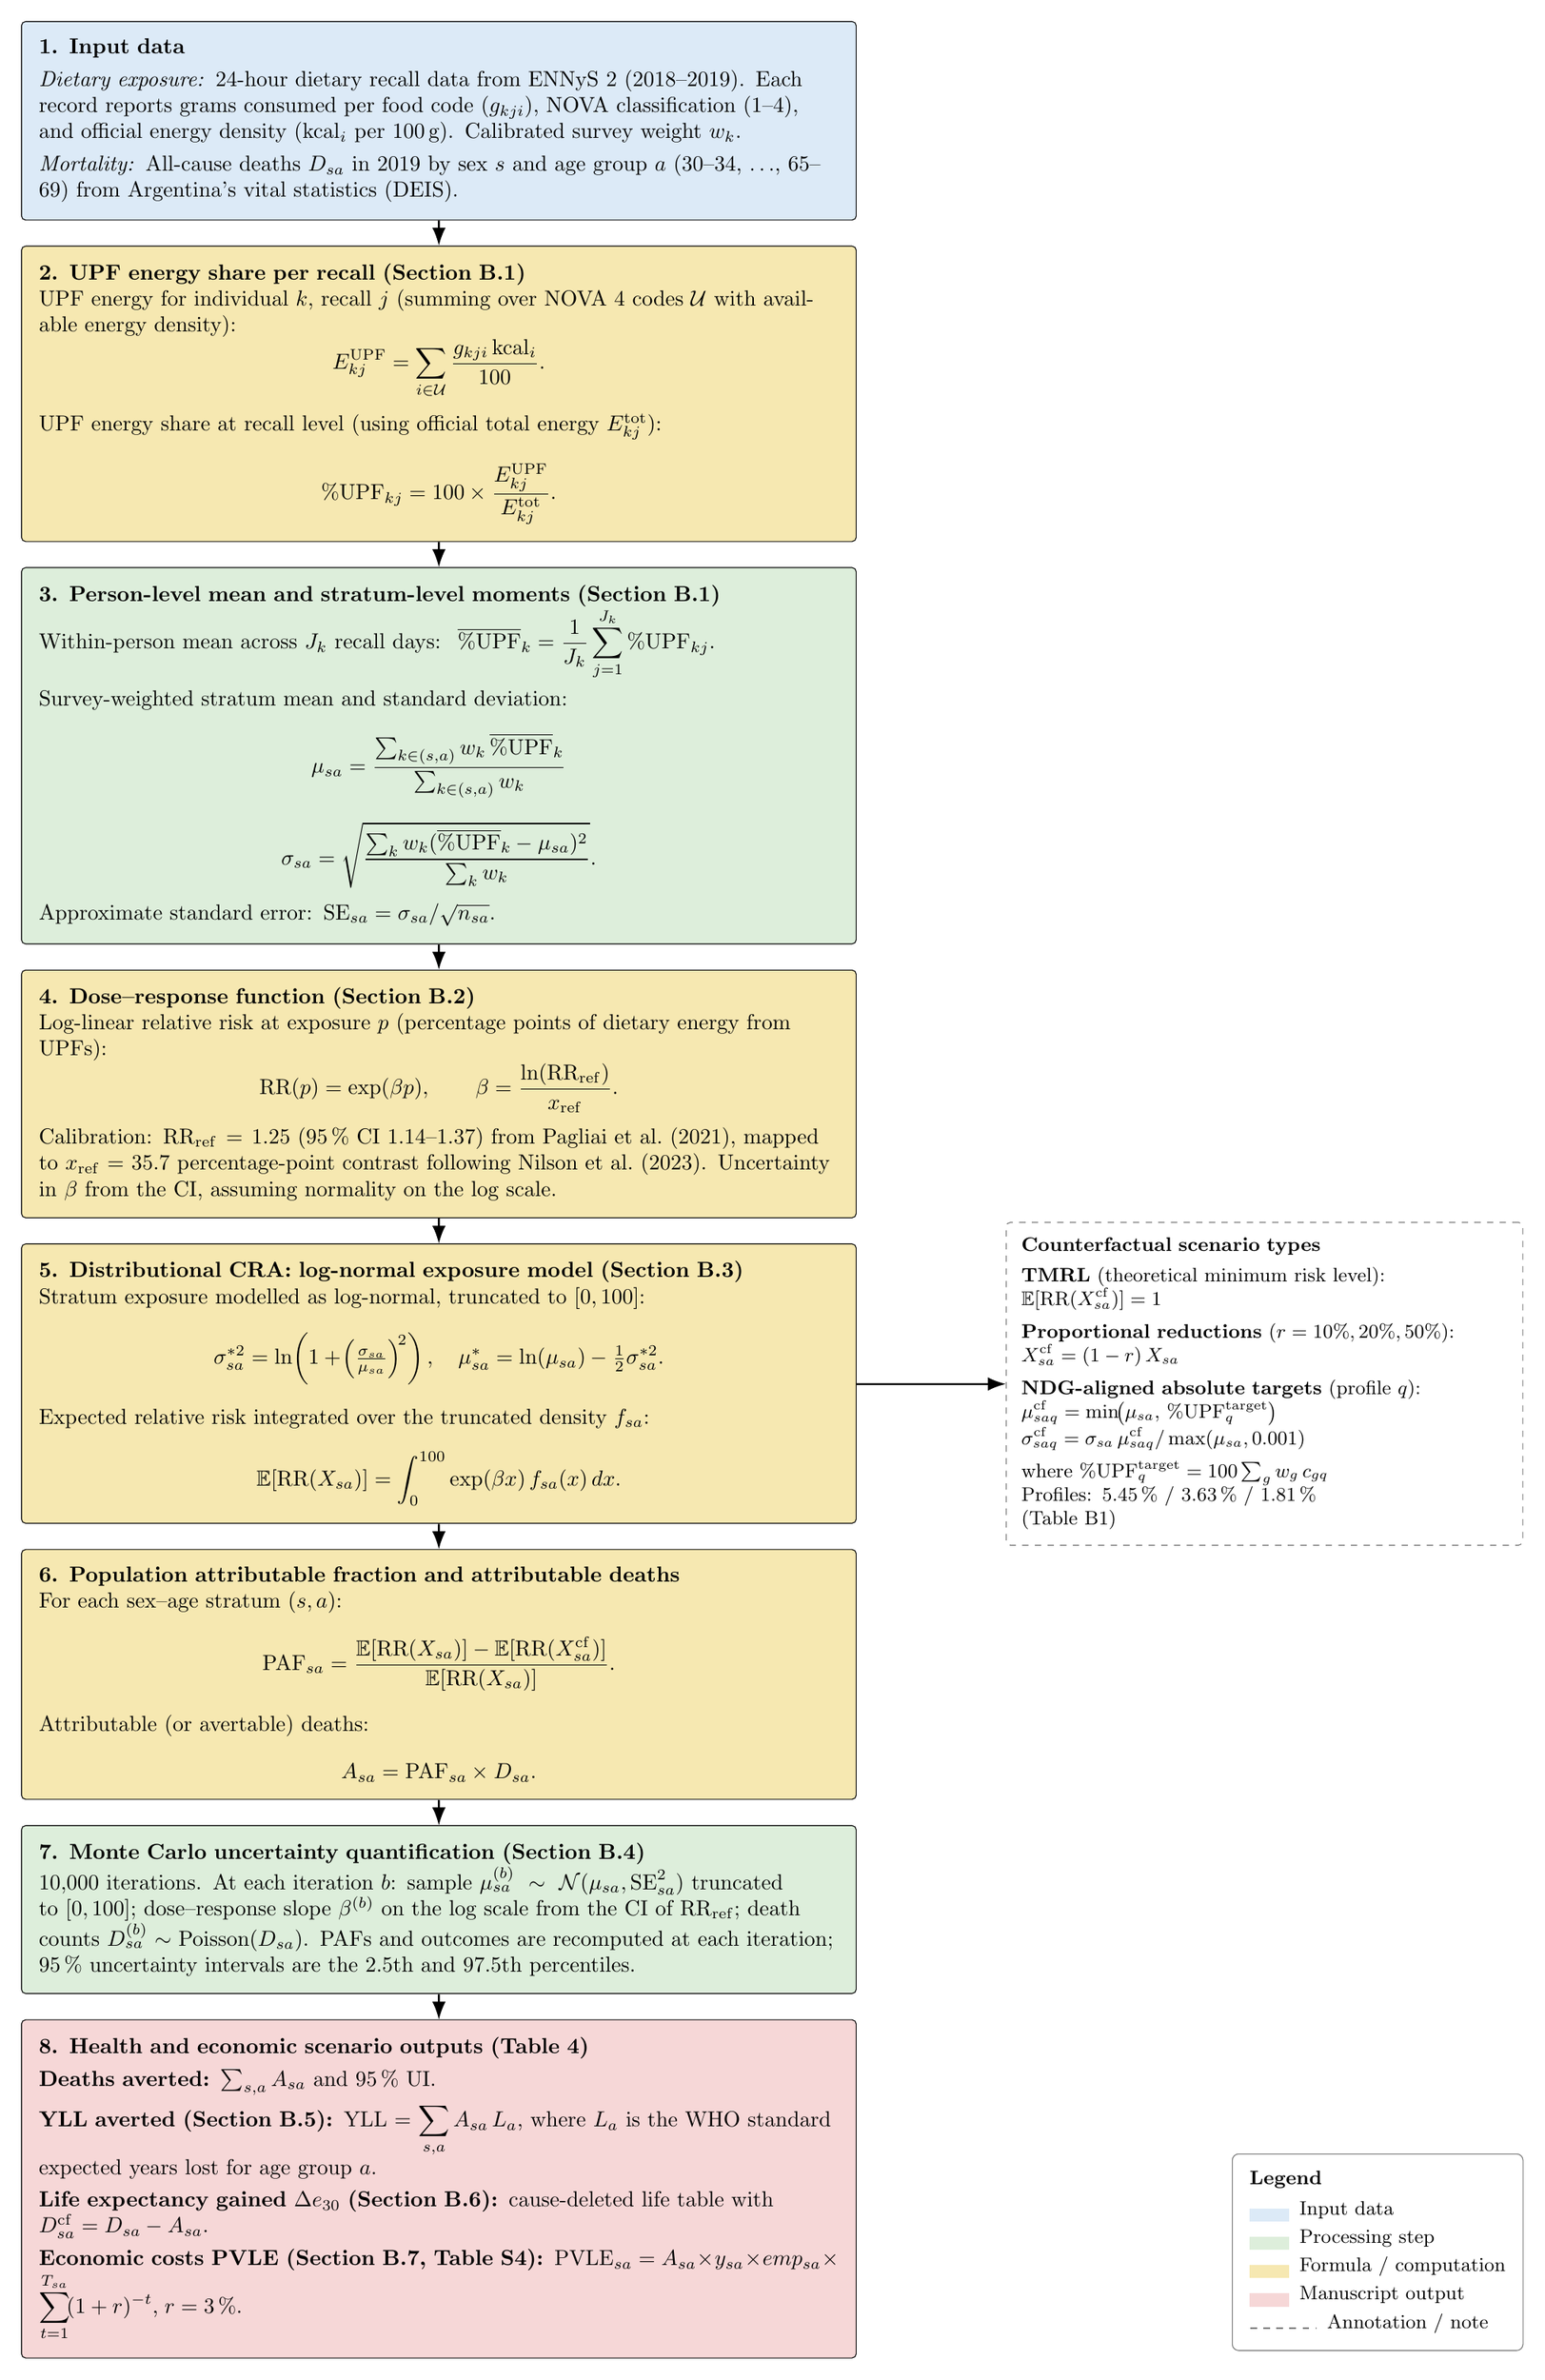
\begin{tikzpicture}[node distance=0.16in and 0.32in, scale=1.03, every node/.style={transform shape}]

\node[data] (input) at (0,0) {
\textbf{1. Input data}\\[3pt]
\textit{Dietary exposure:} 24-hour dietary recall data from ENNyS~2
(2018--2019). Each record reports grams consumed per food code
($g_{kji}$), NOVA classification (1--4), and official energy density
($\mathrm{kcal}_i$ per 100\,g). Calibrated survey weight $w_k$.\\[3pt]
\textit{Mortality:} All-cause deaths $D_{sa}$ in 2019 by sex $s$ and
age group $a$ (30--34, $\ldots$, 65--69) from Argentina's vital
statistics (DEIS).
};

\node[formula, below=of input] (exposure) {
\textbf{2. UPF energy share per recall (Section~B.1)}\\
UPF energy for individual $k$, recall $j$ (summing over NOVA~4 codes
$\mathcal{U}$ with available energy density):
\[
  E^{\mathrm{UPF}}_{kj}=\sum_{i\in\mathcal{U}}\frac{g_{kji}\,\mathrm{kcal}_i}{100}.
\]
UPF energy share at recall level (using official total energy
$E^{\mathrm{tot}}_{kj}$):
\[
  \%\mathrm{UPF}_{kj}=100\times\frac{E^{\mathrm{UPF}}_{kj}}{E^{\mathrm{tot}}_{kj}}.
\]
};

\node[process, below=of exposure] (stratum) {
\textbf{3. Person-level mean and stratum-level moments (Section~B.1)}\\
Within-person mean across $J_k$ recall days:
$\;\overline{\%\mathrm{UPF}}_{k}=\dfrac{1}{J_k}\displaystyle\sum_{j=1}^{J_k}\%\mathrm{UPF}_{kj}$.\\[4pt]
Survey-weighted stratum mean and standard deviation:
\[
  \mu_{sa}=\frac{\sum_{k\in(s,a)}w_k\,\overline{\%\mathrm{UPF}}_{k}}
                {\sum_{k\in(s,a)}w_k}
\]
\[
  \sigma_{sa}=\sqrt{\frac{\sum_{k}w_k(\overline{\%\mathrm{UPF}}_{k}-\mu_{sa})^2}
                         {\sum_{k}w_k}}.
\]
Approximate standard error: $\mathrm{SE}_{sa}=\sigma_{sa}/\sqrt{n_{sa}}$.
};

\node[formula, below=of stratum] (dr) {
\textbf{4. Dose--response function (Section~B.2)}\\
Log-linear relative risk at exposure $p$ (percentage points of
dietary energy from UPFs):
\[
  \mathrm{RR}(p)=\exp(\beta p),\qquad
  \beta=\frac{\ln(\mathrm{RR}_{\mathrm{ref}})}{x_{\mathrm{ref}}}.
\]
Calibration: $\mathrm{RR}_{\mathrm{ref}}=1.25$
(95\,\% CI 1.14--1.37) from Pagliai et~al.\ (2021), mapped to
$x_{\mathrm{ref}}=35.7$ percentage-point contrast following
Nilson et~al.\ (2023). Uncertainty in $\beta$ from the CI, assuming
normality on the log scale.
};

\node[formula, below=of dr] (cra) {
\textbf{5. Distributional CRA: log-normal exposure model (Section~B.3)}\\
Stratum exposure modelled as log-normal, truncated to $[0,100]$:
\[
  \sigma_{sa}^{*2}=\ln\!\left(1+\!\left(\tfrac{\sigma_{sa}}{\mu_{sa}}\right)^{\!2}\right),\quad
  \mu_{sa}^{*}=\ln(\mu_{sa})-\tfrac{1}{2}\sigma_{sa}^{*2}.
\]
Expected relative risk integrated over the truncated density $f_{sa}$:
\[
  \mathbb{E}\!\left[\mathrm{RR}(X_{sa})\right]=\int_0^{100}\exp(\beta x)\,f_{sa}(x)\,dx.
\]
};

\node[note, right=0.95in of cra] (scenarios) {
\textbf{Counterfactual scenario types}\\[3pt]
\textbf{TMRL} (theoretical minimum risk level):\\
$\mathbb{E}[\mathrm{RR}(X^{\mathrm{cf}}_{sa})]=1$\\[4pt]
\textbf{Proportional reductions} ($r=10\%,20\%,50\%$):\\
$X^{\mathrm{cf}}_{sa}=(1-r)\,X_{sa}$\\[4pt]
\textbf{NDG-aligned absolute targets} (profile $q$):\\
$\mu^{\mathrm{cf}}_{saq}=\min\!\bigl(\mu_{sa},\,\%\mathrm{UPF}^{\mathrm{target}}_q\bigr)$\\
$\sigma^{\mathrm{cf}}_{saq}=\sigma_{sa}\,\mu^{\mathrm{cf}}_{saq}/\max(\mu_{sa},0.001)$\\[4pt]
where $\%\mathrm{UPF}^{\mathrm{target}}_q=100\textstyle\sum_g w_g\,c_{gq}$\\
Profiles: 5.45\,\% / 3.63\,\% / 1.81\,\%\\
(Table~B1)
};

\node[formula, below=of cra] (paf) {
\textbf{6. Population attributable fraction and attributable deaths}\\
For each sex--age stratum $(s,a)$:
\[
  \mathrm{PAF}_{sa}=
  \frac{\mathbb{E}[\mathrm{RR}(X_{sa})]-\mathbb{E}[\mathrm{RR}(X^{\mathrm{cf}}_{sa})]}
       {\mathbb{E}[\mathrm{RR}(X_{sa})]}.
\]
Attributable (or avertable) deaths:
\[
  A_{sa}=\mathrm{PAF}_{sa}\times D_{sa}.
\]
};

\node[process, below=of paf] (mc) {
\textbf{7. Monte Carlo uncertainty quantification (Section~B.4)}\\
10,000 iterations. At each iteration $b$: sample
$\mu^{(b)}_{sa}\sim\mathcal{N}(\mu_{sa},\mathrm{SE}_{sa}^2)$ truncated
to $[0,100]$; dose--response slope $\beta^{(b)}$ on the log scale
from the CI of $\mathrm{RR}_{\mathrm{ref}}$; death counts
$D^{(b)}_{sa}\sim\mathrm{Poisson}(D_{sa})$. PAFs and outcomes are
recomputed at each iteration; 95\,\% uncertainty intervals are
the 2.5th and 97.5th percentiles.
};

\node[output, below=of mc] (outputs) {
\textbf{8. Health and economic scenario outputs (Table~4)}\\[3pt]
\textbf{Deaths averted:}\enspace$\sum_{s,a}A_{sa}$ and 95\,\%~UI.\\[3pt]
\textbf{YLL averted (Section~B.5):}\enspace
  $\mathrm{YLL}=\displaystyle\sum_{s,a}A_{sa}\,L_a$,
  where $L_a$ is the WHO standard expected years lost for age group~$a$.\\[3pt]
\textbf{Life expectancy gained} $\Delta e_{30}$ \textbf{(Section~B.6):}
  cause-deleted life table with
  $D^{\mathrm{cf}}_{sa}=D_{sa}-A_{sa}$.\\[3pt]
\textbf{Economic costs PVLE (Section~B.7, Table~S4):}
  $\mathrm{PVLE}_{sa}=A_{sa}\!\times\!y_{sa}\!\times\!emp_{sa}
  \!\times\!\displaystyle\sum_{t=1}^{T_{sa}}\!(1+r)^{-t}$,\;$r=3\,\%$.
};

\node[
  draw=black!55, rounded corners=3pt,
  align=left, inner sep=8pt, font=\small,
  anchor=south east
] (legend) at ($(scenarios.east |- outputs.south)+(0.00in,0.05in)$) {
  \textbf{Legend}\\[3pt]
  \colorbox{FlowBlue}{\hphantom{~~~~}}\enspace Input data\\[2pt]
  \colorbox{FlowGreen}{\hphantom{~~~~}}\enspace Processing step\\[2pt]
  \colorbox{FlowYellow}{\hphantom{~~~~}}\enspace Formula / computation\\[2pt]
  \colorbox{FlowRed}{\hphantom{~~~~}}\enspace Manuscript output\\[2pt]
  \tikz[baseline=0pt]\draw[black!55,dashed,line width=0.7pt](0,0)--(0.42in,0);%
  \enspace Annotation / note
};

\draw[flow]      (input)    -- (exposure);
\draw[flow]      (exposure) -- (stratum);
\draw[flow]      (stratum)  -- (dr);
\draw[flow]      (dr)       -- (cra);
\draw[smallflow] (cra)      -- (scenarios);
\draw[flow]      (cra)      -- (paf);
\draw[flow]      (paf)      -- (mc);
\draw[flow]      (mc)       -- (outputs);

\end{tikzpicture}
\end{adjustbox}%
}
\manualfigurecaption{\textbf{Fig S1.} Flow diagram of health impact estimation. Blue\,=\,input data; green\,=\,processing; yellow\,=\,formula/computation; red\,=\,manuscript output. Note: solid arrows indicate the main computational sequence, while dashed arrows indicate auxiliary annotations. Section and table references point to this appendix.}
\end{figure}

\clearpage

\begin{figure}[p]
\centering
\makebox[\textwidth][c]{%
{%
\tikzset{
  box/.append style={text width=5.35in, inner sep=9pt},
  note/.append style={text width=3.25in, font=\normalsize}
}
\begin{adjustbox}{width=1.30\textwidth, totalheight=0.985\textheight, keepaspectratio}
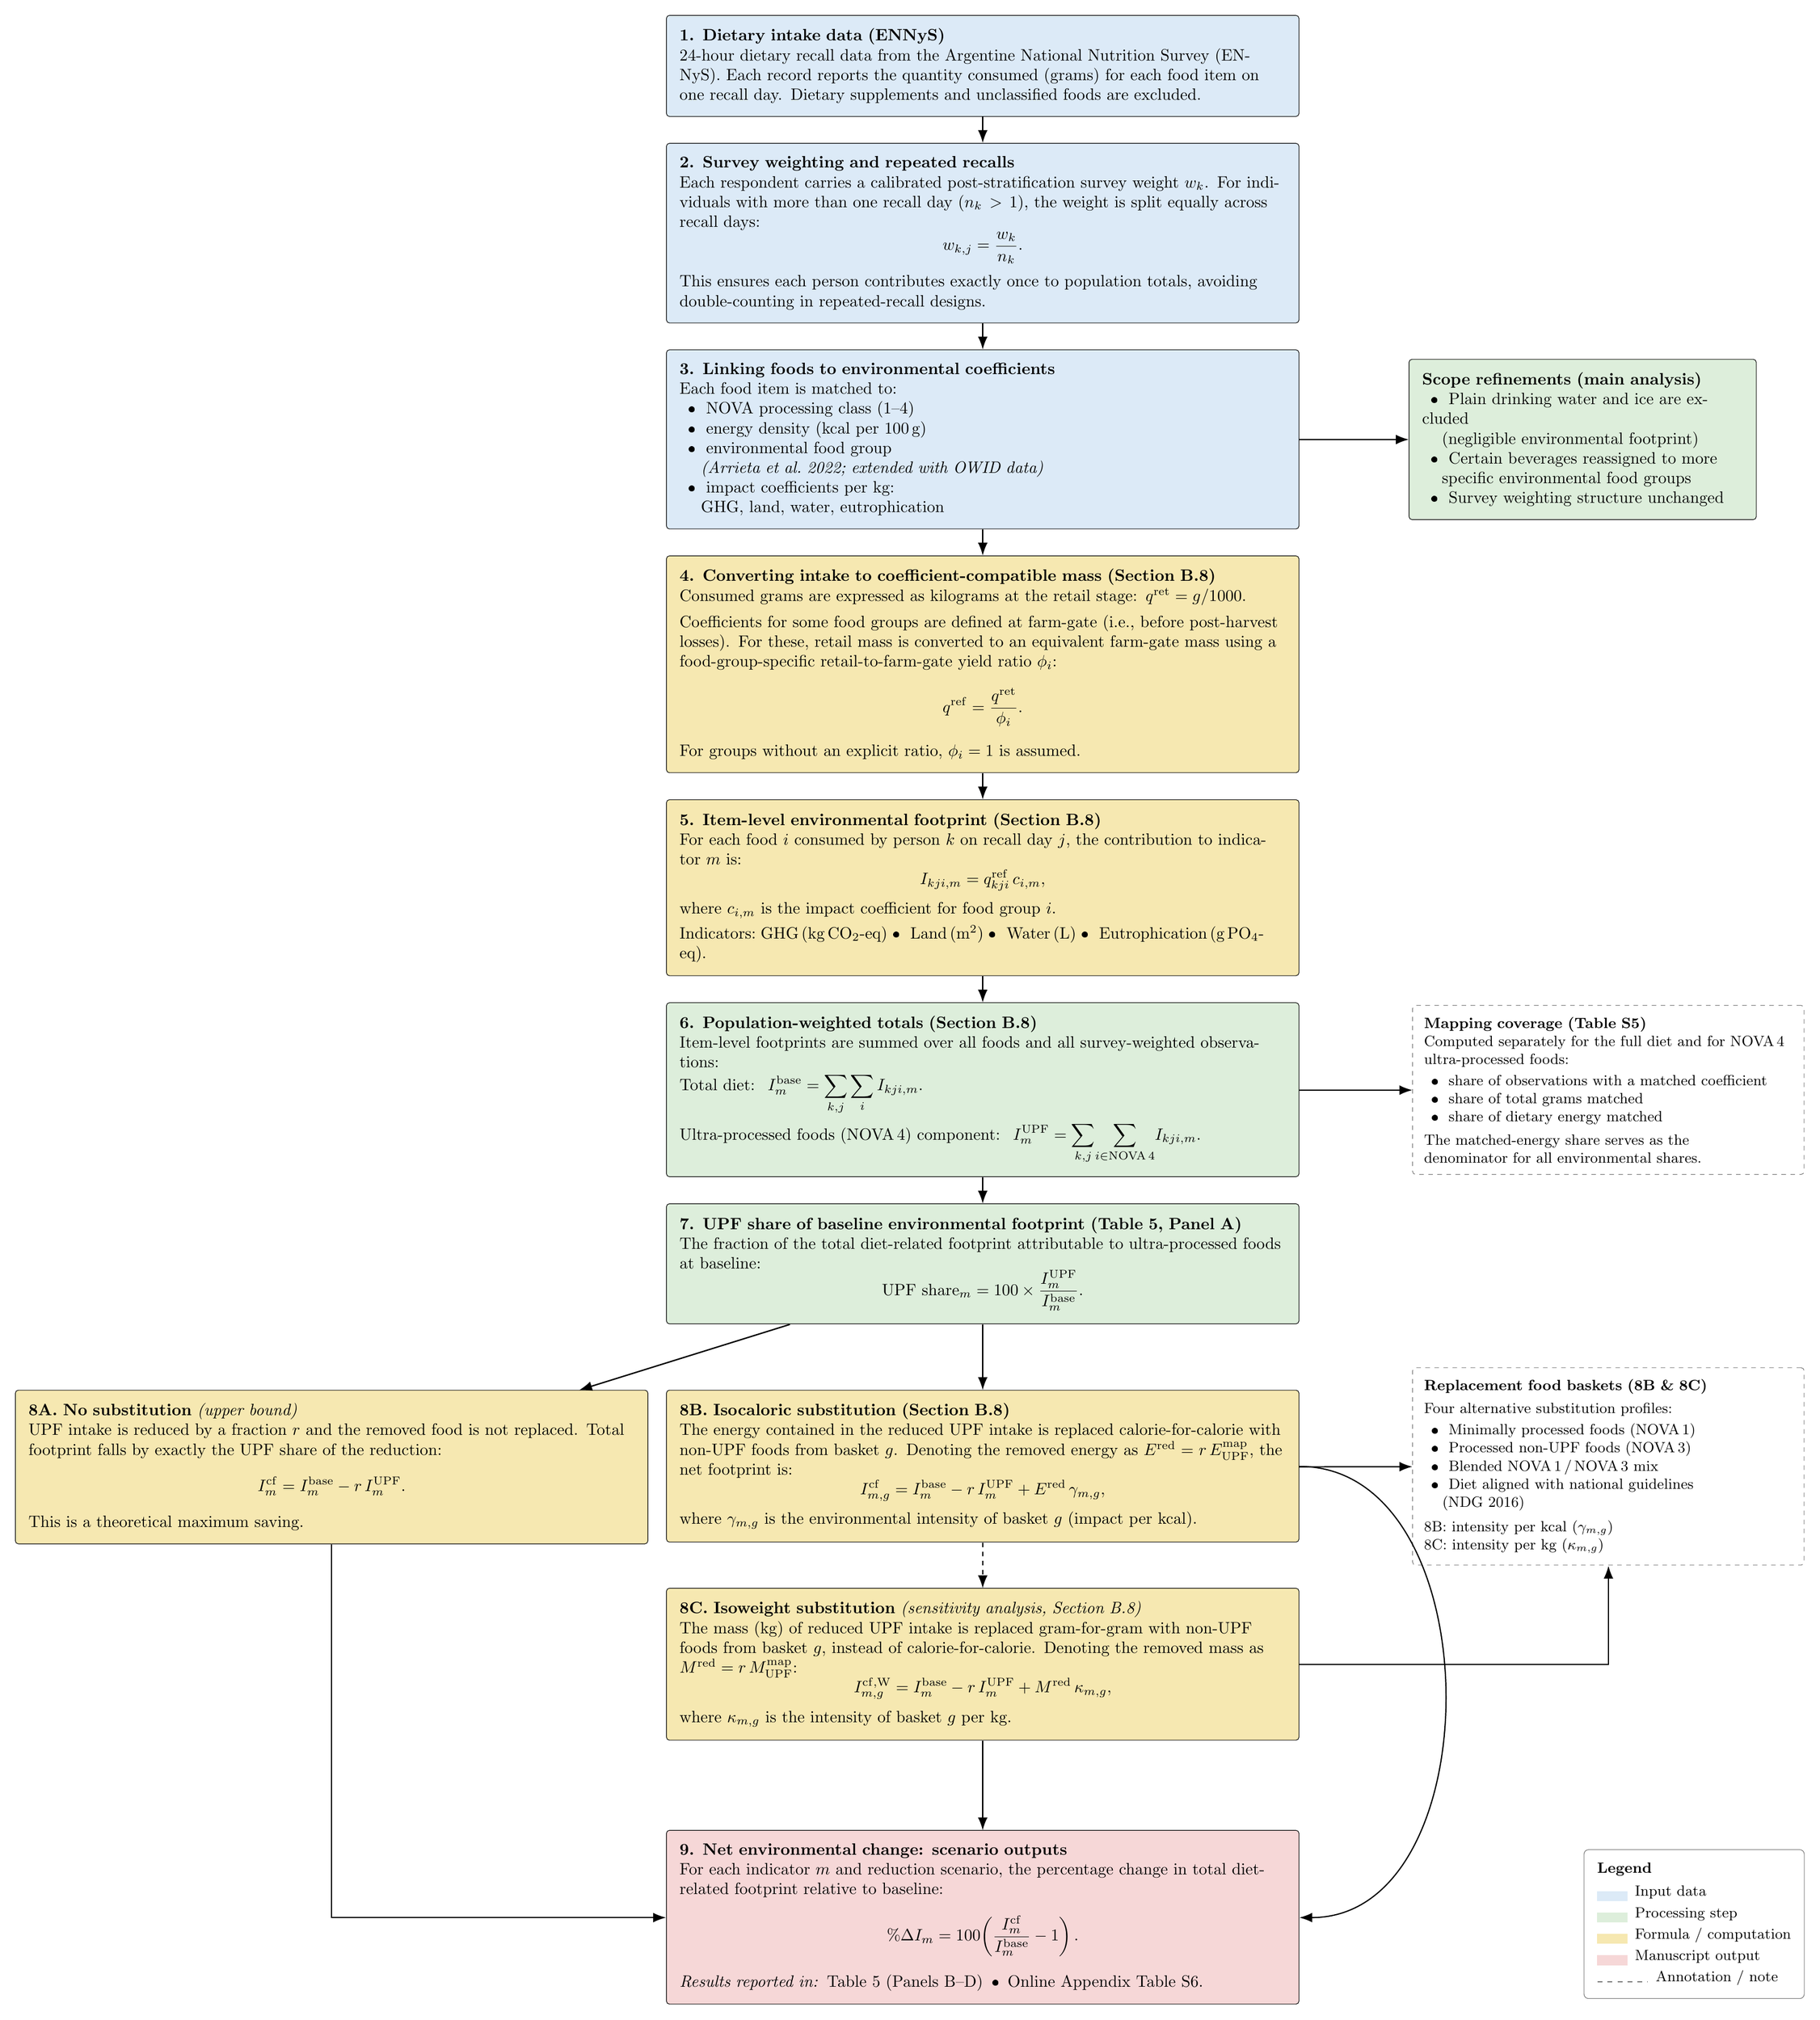
\begin{tikzpicture}[node distance=0.22in and 0.34in, scale=1.09, every node/.style={transform shape}]

\node[data] (input) at (0,0) {
\textbf{1. Dietary intake data (ENNyS)}\\
24-hour dietary recall data from the Argentine National Nutrition
Survey (ENNyS). Each record reports the quantity consumed (grams)
for each food item on one recall day. Dietary supplements and
unclassified foods are excluded.
};

\node[data, below=of input] (weights) {
\textbf{2. Survey weighting and repeated recalls}\\
Each respondent carries a calibrated post-stratification survey
weight~$w_k$. For individuals with more than one recall day ($n_k>1$),
the weight is split equally across recall days:
\[
  w_{k,j}=\frac{w_k}{n_k}.
\]
This ensures each person contributes exactly once to population totals,
avoiding double-counting in repeated-recall designs.
};

\node[data, below=of weights] (joins) {
\textbf{3. Linking foods to environmental coefficients}\\
Each food item is matched to:\\
\hspace*{0.5em}\textbullet\; NOVA processing class (1--4)\\
\hspace*{0.5em}\textbullet\; energy density (kcal per 100\,g)\\
\hspace*{0.5em}\textbullet\; environmental food group\\
\hspace*{1.3em}\textit{(Arrieta et~al.\ 2022; extended with OWID data)}\\
\hspace*{0.5em}\textbullet\; impact coefficients per kg:\\
\hspace*{1.3em}GHG, land, water, eutrophication
};

\node[process, right=0.92in of joins, text width=2.70in] (curated) {
\textbf{Scope refinements (main analysis)}\\
\hspace*{0.5em}\textbullet\; Plain drinking water and ice are excluded\\
\hspace*{1.2em}(negligible environmental footprint)\\
\hspace*{0.5em}\textbullet\; Certain beverages reassigned to more\\
\hspace*{1.2em}specific environmental food groups\\
\hspace*{0.5em}\textbullet\; Survey weighting structure unchanged
};

\node[formula, below=of joins] (mass) {
\textbf{4. Converting intake to coefficient-compatible mass (Section~B.8)}\\
Consumed grams are expressed as kilograms at the retail stage:
$q^{\mathrm{ret}}=g/1000$.\\[4pt]
Coefficients for some food groups are defined at farm-gate (i.e.,
before post-harvest losses). For these, retail mass is converted to
an equivalent farm-gate mass using a food-group-specific
retail-to-farm-gate yield ratio~$\phi_i$:
\[
  q^{\mathrm{ref}}=\frac{q^{\mathrm{ret}}}{\phi_i}.
\]
For groups without an explicit ratio, $\phi_i=1$ is assumed.
};

\node[formula, below=of mass] (itemimpact) {
\textbf{5. Item-level environmental footprint (Section~B.8)}\\
For each food~$i$ consumed by person~$k$ on recall day~$j$, the
contribution to indicator~$m$ is:
\[
  I_{kji,m}=q^{\mathrm{ref}}_{kji}\,c_{i,m},
\]
where $c_{i,m}$ is the impact coefficient for food group~$i$.\\[3pt]
Indicators:\;GHG\,(kg\,CO$_2$-eq)\;\textbullet\;
Land\,(m$^2$)\;\textbullet\;
Water\,(L)\;\textbullet\;
Eutrophication\,(g\,PO$_4$-eq).
};

\node[process, below=of itemimpact] (aggregate) {
\textbf{6. Population-weighted totals (Section~B.8)}\\
Item-level footprints are summed over all foods and all
survey-weighted observations:\\[2pt]
Total diet:\;
$\displaystyle I^{\mathrm{base}}_m=\sum_{k,j}\sum_i I_{kji,m}$.\\[4pt]
Ultra-processed foods (NOVA\,4) component:\;
$\displaystyle I^{\mathrm{UPF}}_m=\sum_{k,j}\!\sum_{i\in\mathrm{NOVA\,4}}\! I_{kji,m}$.
};

\node[note, right=0.95in of aggregate] (coverage) {
\textbf{Mapping coverage (Table~S5)}\\
Computed separately for the full diet and for NOVA\,4
ultra-processed foods:\\[2pt]
\hspace*{0.5em}\textbullet\; share of observations with a matched coefficient\\
\hspace*{0.5em}\textbullet\; share of total grams matched\\
\hspace*{0.5em}\textbullet\; share of dietary energy matched\\[3pt]
The matched-energy share serves as the\\
denominator for all environmental shares.
};

\node[process, below=of aggregate] (shares) {
\textbf{7. UPF share of baseline environmental footprint (Table~5, Panel~A)}\\
The fraction of the total diet-related footprint attributable to
ultra-processed foods at baseline:
\[
  \text{UPF share}_m = 100\times\frac{I^{\mathrm{UPF}}_m}{I^{\mathrm{base}}_m}.
\]
};

\node[formula, below left=0.55in and 0.15in of shares] (norepl) {
\textbf{8A. No substitution} \normalfont\textit{(upper bound)}\\
UPF intake is reduced by a fraction~$r$ and the removed
food is not replaced. Total footprint falls by exactly the
UPF share of the reduction:
\[
  I^{\mathrm{cf}}_m = I^{\mathrm{base}}_m - r\,I^{\mathrm{UPF}}_m.
\]
This is a theoretical maximum saving.
};

\node[formula, below=0.55in of shares] (iso) {
\textbf{8B. Isocaloric substitution (Section~B.8)}\\
The energy contained in the reduced UPF intake is replaced
calorie-for-calorie with non-UPF foods from basket~$g$.
Denoting the removed energy as $E^{\mathrm{red}}=r\,E^{\mathrm{map}}_{\mathrm{UPF}}$,
the net footprint is:
\[
  I^{\mathrm{cf}}_{m,g}=I^{\mathrm{base}}_m-r\,I^{\mathrm{UPF}}_m
  +E^{\mathrm{red}}\,\gamma_{m,g},
\]
where $\gamma_{m,g}$ is the environmental intensity of basket~$g$
(impact per kcal).
};

\node[note, right=0.95in of iso] (baskets) {
\textbf{Replacement food baskets (8B \& 8C)}\\[3pt]
Four alternative substitution profiles:\\[2pt]
\hspace*{0.5em}\textbullet\; Minimally processed foods (NOVA\,1)\\
\hspace*{0.5em}\textbullet\; Processed non-UPF foods (NOVA\,3)\\
\hspace*{0.5em}\textbullet\; Blended NOVA\,1\,/\,NOVA\,3 mix\\
\hspace*{0.5em}\textbullet\; Diet aligned with national guidelines\\
\hspace*{1.2em}(NDG~2016)\\[4pt]
8B: intensity per kcal ($\gamma_{m,g}$)\\
8C: intensity per kg ($\kappa_{m,g}$)
};

\node[formula, below=0.38in of iso] (isoweight) {
\textbf{8C. Isoweight substitution}
\normalfont\textit{(sensitivity analysis, Section~B.8)}\\
The mass (kg) of reduced UPF intake is replaced gram-for-gram
with non-UPF foods from basket~$g$, instead of calorie-for-calorie.
Denoting the removed mass as $M^{\mathrm{red}}=r\,M^{\mathrm{map}}_{\mathrm{UPF}}$:
\[
  I^{\mathrm{cf,W}}_{m,g}=I^{\mathrm{base}}_m-r\,I^{\mathrm{UPF}}_m
  +M^{\mathrm{red}}\,\kappa_{m,g},
\]
where $\kappa_{m,g}$ is the intensity of basket~$g$ per kg.
};

\node[output, below=0.75in of isoweight] (outputs) {
\textbf{9. Net environmental change: scenario outputs}\\
For each indicator~$m$ and reduction scenario, the percentage change
in total diet-related footprint relative to baseline:
\[
  \%\Delta I_m = 100\!\left(\frac{I^{\mathrm{cf}}_m}{I^{\mathrm{base}}_m}-1\right).
\]
\textit{Results reported in:}\enspace
Table~5 (Panels~B--D)\enspace\textbullet\enspace
Online Appendix Table~S6.
};

\node[
  draw=black!55, rounded corners=3pt,
  align=left, inner sep=8pt, font=\small,
  anchor=south east
] (legend2) at ($(baskets.east |- outputs.south)+(0.00in,0.05in)$) {
  \textbf{Legend}\\[3pt]
  \colorbox{FlowBlue}{\hphantom{~~~~}}\enspace Input data\\[2pt]
  \colorbox{FlowGreen}{\hphantom{~~~~}}\enspace Processing step\\[2pt]
  \colorbox{FlowYellow}{\hphantom{~~~~}}\enspace Formula / computation\\[2pt]
  \colorbox{FlowRed}{\hphantom{~~~~}}\enspace Manuscript output\\[2pt]
  \tikz[baseline=0pt]\draw[black!55,dashed,line width=0.7pt](0,0)--(0.42in,0);%
  \enspace Annotation / note
};

\draw[flow]      (input)      -- (weights);
\draw[flow]      (weights)    -- (joins);
\draw[smallflow] (joins)      -- (curated);
\draw[flow]      (joins)      -- (mass);
\draw[flow]      (mass)       -- (itemimpact);
\draw[flow]      (itemimpact) -- (aggregate);
\draw[smallflow] (aggregate)  -- (coverage);
\draw[flow]      (aggregate)  -- (shares);
\draw[flow]      (shares)     -- (norepl);
\draw[flow]      (shares)     -- (iso);
\draw[smallflow] (iso)        -- (baskets);
\draw[smallflow, dashed] (iso) -- (isoweight);
\draw[smallflow] (isoweight.east) -| (baskets.south);
\draw[smallflow] (norepl.south)    |- (outputs.west);
\draw[smallflow] (iso.east) to[out=0,in=0,looseness=1.1] (outputs.east);
\draw[flow]      (isoweight)       -- (outputs);

\end{tikzpicture}
\end{adjustbox}%
}%
}
\manualfigurecaption{\textbf{Fig S2.} Flow diagram of environmental impact estimation. Blue\,=\,input data; green\,=\,processing; yellow\,=\,formula/computation; red\,=\,manuscript output. Note: the dashed arrow from 8B to 8C indicates that isoweight substitution is a sensitivity variant, not a sequential step.}
\end{figure}

\clearpage
\nocite{Monteiro2019UPFIdentify,Pagliai2021,Nilson2023,WHO2024MethodsGBD,ENNYS22019,INDECEPH2019Q4,WorldBankPPP2019,Arrieta2022SustainSci,PooreNemecek2018,OWIDDatasets2026,ADEMEAgribalyse2026}
\IfFileExists{references_upf_argentina.bib}{%
\bibliography{references_upf_argentina}%
}{%
\bibliography{output/references_upf_argentina}%
}

\end{document}


